\documentclass[oneside]{book}
\usepackage{ifthen, tikz}
\usepackage{lipsum} % for generating dummy text
\usepackage{xparse}
\usepackage{amsmath}
\usepackage{amsfonts}
\usepackage{placeins}
\usepackage[T1]{fontenc}
\usepackage{import}
\usepackage{graphicx}
\usepackage{adjustbox}

\usepackage{geometry}
\geometry{hmargin=4cm,vmargin=4cm}

\allowdisplaybreaks



\usetikzlibrary {arrows.meta,automata,positioning,shadows,decorations.pathmorphing, decorations.pathreplacing, decorations.shapes, graphs, calc, math}
\usetikzlibrary{shapes.geometric}
\usetikzlibrary{decorations.pathreplacing}
\usetikzlibrary {arrows.meta}


\tikzset{%
   dot/.style={
      circle,
      inner sep=0mm,
      outer sep=0mm,
      minimum size=2mm,
      draw=black,
      fill=black
   },
    triple/.style={
      double distance=2pt,
      postaction={draw}
    },
    quadruple/.style={
      double,
      double distance=2pt,
      postaction={
        draw,
        transform canvas={yshift=-.4pt},
      },
      postaction={
        draw,
        transform canvas={yshift=.4pt},
      }
    },
   every loop/.style={},
   d/.style={
     Circle[]-,
     shorten <=-2pt,
     transform canvas={shift={(-3pt, 4pt)}}
   },
   d0/.style={
     Circle[]-,
     shorten <=-2pt,
   },
   d1/.style={
     Circle[]-,
   },
   dn/.style={
     draw, circle, minimum size=1.3em
   },
   ddn/.style={
     draw, circle, double, minimum size=1.3em
   },
   dddn/.style={
     draw, circle, double, minimum size=1.3em,
       double distance=2pt,
       postaction={draw}
   },
   triangle/.style={
    regular polygon,
    regular polygon sides=3,
    rotate=270,
    scale=.5,
    inner sep=3pt,
    draw
   },
}



\newcommand{\trace}[2]{% #1 is the list of items, #2 is the looseness for the loop
   %\pgfmathsetmacro{\negspace}{-1.0em - 0.5em*#2} % Calculate negative space
   \hspace{-1em}
    \begin{tikzpicture}[baseline=(node1.base), inner sep=1pt]
        % Initialize a counter for tracking the number of items
        \newcount\itemcount
        \itemcount=0
        
        % Define nodes
        \def\lastnode{node1}
        \foreach \i [count=\c] in {#1} {
            \ifnum \c=1
                \node (node\c) {$\i$}; % First node
            \else
                \node[right=1em of \lastnode] (node\c) {$\i$}; % Subsequent nodes
                \draw (\lastnode) -- (node\c); % Draw edge from last node to current
            \fi
            \global\advance\itemcount by 1
            \xdef\lastnode{node\c}
        }
        
        % Draw the loop edge
        \ifnum \itemcount=1
            \path (node1) edge [out=160, in=20, loop] ();
        \else
            \path (node1) edge [out=160, in=20, looseness=#2] (\lastnode);
        \fi
    \end{tikzpicture}
   \hspace{-1em}
}

\def\matmul#1{
   \vecmatvec{.5em}{}{#1}{}
}

\def\vecmatvec#1#2#3#4{
   \begin{tikzpicture}[baseline=-.25em, inner sep=1pt]
      \node (node0) {$#2$};
      \xdef\lastnode{node0};
      \foreach \i [count=\c] in {#3} {
         \node[right=#1 of \lastnode] (node\c) {$\i$};
         \draw (\lastnode.east) -- (node\c);
         \xdef\lastnode{node\c};
      }
      \node[right=#1 of \lastnode] (last) {$#4$};
      \draw (\lastnode.east) -- (last);
   \end{tikzpicture}
}

\def\detstack#1{
   \mathbin{\begin{tikzpicture}[baseline=(a0.base), inner sep=1pt]
      \node (a0) {#1};
      \node[right=.5em of a0] (dots) {$\cdots$};
      \node[right=.5em of dots] (a1) {#1};
      \draw (a0.north) -- ++(0,.2) coordinate (a0top);
      \draw (a1.north) -- ++(0,.2) coordinate (a1top);
      \draw (a0.south) -- ++(0,-.2) coordinate (a0bot);
      \draw (a1.south) -- ++(0,-.2) coordinate (a1bot);
      \draw[line width=2pt] (a0top -| a0.west) -- (a1top -| a1.east);
      \draw[line width=2pt] (a0bot -| a0.west) -- (a1bot -| a1.east);
   \end{tikzpicture}}
}

% Define a new command for drawing the ellipse
\NewDocumentCommand{\drawellipse}{m m m m m o}{
    \def\centerX{#1}
    \def\centerY{#2}
    \def\widthR{#3}
    \def\heightR{#4}
    \def\angle{#5}
    
    \draw (\centerX,\centerY) ellipse [x radius=\widthR, y radius=\heightR];
    \fill ({\centerX + \widthR*cos(\angle)},{\centerY + \heightR*sin(\angle)}) circle [radius=0.075];
    
    % If target node is provided, use it, otherwise fall back to default behavior
    \IfNoValueTF{#6}{
        \draw ({\centerX + \widthR*cos(\angle)},{\centerY + \heightR*sin(\angle)}) -- ({\centerX + .5 + \widthR*cos(\angle)}, {\centerY + \heightR*sin(\angle)});
    }{
        \draw ({\centerX + \widthR*cos(\angle)},{\centerY + \heightR*sin(\angle)}) -- (#6);
    }
}


\newcommand{\smat}[1]{\left[\begin{smallmatrix}#1\end{smallmatrix}\right]}
\newcommand{\svec}[1]{[\begin{smallmatrix}#1\end{smallmatrix}]}
\newcommand{\E}{\mathrm{E}}
% \newcommand\sbullet[1][.5]{\mathbin{\hbox{\scalebox{#1}{$\bullet$}}}}
\newcommand\sbullet[1][1.5pt]{%
  \tikz[baseline=-0.5ex]\draw (0,0) circle (#1);%
}
\newcommand{\R}{\mathbb R}
\newcommand{\eps}{\varepsilon}


\title{The Tensor Cookbook}
\author{Thomas Dybdahl Ahle}
\begin{document}

% Consider also taking some inspiration from https://arxiv.org/pdf/1802.01528
% "The Matrix Calculus You Need For Deep Learning"

\maketitle


\chapter{Introduction}
\paragraph{What is this?}
These pages are a guide to tensors, using the visual language of ``ensor diagrams''.
For illustrating the generality of the approach, I've tried to closely follow the legendary ``Matrix Cookbook''.
As such, most of the presentation is a collection of facts (identities, approximations, inequalities, relations, ...) about tensors and matters relating to them.
You won't find many results not in the original cookbook, but hopefully the diagrams will give you a new way to understand and appreciate them.

\paragraph{It's ongoing:}
The Matrix Cookbook is a long book, and not all the sections are equally amendable to diagrams.
Hence I've opted to skip certain sections and shorten others.
Perhaps in the future, I, or others, will expand the coverage further.

For example, while we cover all of the results on Expectation of Linear Combinations and Gaussian moments, we skip the section on general multi-variate distributions.
I have also had to rearrange the material a bit, to avoid having to introduce all the notation up front.

\paragraph{Complex Matrices and Covariance}
Tensor diagrams (or networks) are currently most often seen in Quantum Physics.
Here most values are complex numbers, which introduce some extra complexity.
In particular transposing a matrix now involves taking the conjugate (flipping the sign of the imaginary part), which introduces the need for co- and contra-variant tensors.
None of this complexity is present with standard real valued matrices, as is common e.g. in Machine Learning applications.
For simplicity I have decided to not include these complexities.

\paragraph{Tensorgrad}
The symbolic nature of tensor diagrams make the well suited for symbolic computation.

\paragraph{Advantages of Tensor Diagram Notation:}
Tensor diagram notation has many benefits compared to other notations:

Various operations, such as a trace, tensor product, or tensor contraction can be expressed simply without extra notation.
Names of indices and tensors can often be omitted. This saves time and lightens the notation, and is especially useful for internal indices which exist mainly to be summed over.
The order of the tensor resulting from a complicated network of contractions can be determined by inspection: it is just the number of unpaired lines. For example, a tensor network with all lines joined, no matter how complicated, must result in a scalar.


\paragraph{Etymology}
The term "tensor" is rooted in the Latin word tensio, meaning ``tension'' or ``stretching,'' derived from the verb tendere, which means ``to stretch'' or ``to extend.''
It was first introduced in the context of mathematics in the mid-19th century by William Rowan Hamilton in his work on quaternions, where it referred to the magnitude of a quaternion.
The modern usage of "tensor" was later established by Gregorio Ricci-Curbastro and Tullio Levi-Civita in their development of tensor calculus, a framework that generalizes the concept of scalars, vectors, and matrices to more complex, multidimensional entities.~\cite{tensor_etymology_russo, hamilton_tensor}.


\tableofcontents
\clearpage

\section{Notation and Nomenclature}
\[
   [P] = \begin{cases}
      1 \text{ if } P \\
      0 \text{ otherwise}
   \end{cases}.
\]

\section{Tensor Diagrams}
Tensor diagrams are simple graphs (or ``networks'') where
nodes represent variables (e.g. vectors or matrices) and edges represent
contractions (e.g. matrix multiplication or inner products.)
The follow table shows how some basic operations can be written with tensor diagrams:

\newenvironment{compress}{
  \renewcommand{\arraystretch}{0.6} % Set the array stretch
  \setlength{\arraycolsep}{2pt}     % Set the column separation
  \vspace{.3em}
}{
  \vspace{.3em}
  \renewcommand{\arraystretch}{1}   % Reset to default after the environment
  \setlength{\arraycolsep}{5pt}     % Reset to default column separation
}

\renewcommand{\arraystretch}{2}
\noindent
%\hspace{-1em}
\vspace{.5em}
\begin{tabular}[h]{lcccl}
   Dot product
   &
   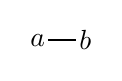
\begin{tikzpicture}[baseline=(a0.base), inner sep=1pt]
      \node (a0) {$a$};
      \node[right=1em of a0] (a1) {$b$};
      \path (a0) edge (a1);
   \end{tikzpicture}
   &
   $y=\sum_i a_i b_i$
   &
   $
\begin{compress}
\left[\begin{array}{cccc}
\cdot & \cdot & \cdot & \cdot \\
\end{array}\right]
\left[\begin{array}{c}
\cdot \\
\cdot \\
\cdot \\
\cdot \\
\end{array}\right]
\end{compress}
   $
   &
   $=y$
   \\
   Outer product
   &
   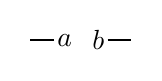
\begin{tikzpicture}[baseline=(a0.base), inner sep=1pt]
      \node (a0) {$a$};
      \node[right=.5em of a0] (a1) {$b$};
      \draw (a0.west) -- ++(-.3,0) node {};
      \draw (a1.east) -- ++(.3,0) node {};
   \end{tikzpicture}
   &
   $Y_{i,j} = a_i b_j$
   &
   $
\begin{compress}
\left[\begin{array}{c}
\cdot \\
\cdot \\
\cdot \\
\cdot \\
\end{array}\right]
\left[\begin{array}{cccc}
\cdot & \cdot & \cdot & \cdot \\
\end{array}\right]
\end{compress}
   $
   &
   $=\mathbin{
   \begin{tikzpicture}[baseline=(Y.base), inner sep=1pt]
      \node (Y) {$Y$};
      \draw (Y.east) -- ++(.3, 0);
      \draw (Y.west) -- ++(-.3, 0);
   \end{tikzpicture}}
   $
   \\
   Matrix-Vector
   &
   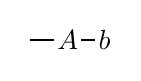
\begin{tikzpicture}[baseline=(A.base), inner sep=1pt]
      \node (A) {$A$};
      \node[right=.5em of A] (b) {$b$};
      \draw (A.west) -- ++(-.3,0) node {};
      \draw (A.east) -- (b.west);
   \end{tikzpicture}
   &
   $
   y_{i} = \sum_j A_{i,j} b_j
   $
   &
   $
   \begin{compress}
   \left[\begin{array}{cccc}
   \cdot & \cdot & \cdot & \cdot \\
   \cdot & \cdot & \cdot & \cdot \\
   \cdot & \cdot & \cdot & \cdot \\
   \cdot & \cdot & \cdot & \cdot \\
   \end{array}\right]
   \left[\begin{array}{c}
   \cdot \\
   \cdot \\
   \cdot \\
   \cdot \\
   \end{array}\right]
   \end{compress}
   $
   &
   $=\mathbin{
   \begin{tikzpicture}[baseline=(y.base), inner sep=1pt]
      \node (y) {$y$};
      \draw (y.west) -- ++(-.3, 0);
   \end{tikzpicture}
   }$
   \\
   Matrix-Matrix
   &
   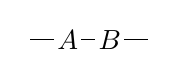
\begin{tikzpicture}[baseline=(A.base), inner sep=1pt]
      \node (A) {$A$};
      \node[right=.5em of A] (B) {$B$};
      \draw (A.west) -- ++(-.3,0) node {};
      \draw (A.east) -- (B.west);
      \draw (B.east) -- ++(.3,0) node {};
   \end{tikzpicture}
   &
   $
   Y_{i,k} = \sum_j A_{i,j} B_{j,k}
   $
   &
   $
   \begin{compress}
   \left[\begin{array}{cccc}
   \cdot & \cdot & \cdot & \cdot \\
   \cdot & \cdot & \cdot & \cdot \\
   \cdot & \cdot & \cdot & \cdot \\
   \cdot & \cdot & \cdot & \cdot \\
   \end{array}\right]
   \left[\begin{array}{cccc}
   \cdot & \cdot & \cdot & \cdot \\
   \cdot & \cdot & \cdot & \cdot \\
   \cdot & \cdot & \cdot & \cdot \\
   \cdot & \cdot & \cdot & \cdot \\
   \end{array}\right]
   \end{compress}
   $
   &
   $=\mathbin{
   \begin{tikzpicture}[baseline=(Y.base), inner sep=1pt]
      \node (Y) {$Y$};
      \draw (Y.west) -- ++(-.3, 0);
      \draw (Y.east) -- ++(.3, 0);
   \end{tikzpicture}
   }$
\end{tabular}
\vspace{.5em}

We think of vectors and matrices as tensors of order 1 and 2.
The order corresponds to the number of dimensions in their $[\cdots]$ visualization above,
e.g. a vector is a 1-dimensional list of numbers, while a matrix is a 2-dimensional grid of numbers.
The order also determines the degree of the node representing the variable in the tensor graph.

Diagram notation becomes more interesting when you have tensors of order 3 and higher.
An order 3 tensor is a cube or numbers, or stack of matrices.
E.g. we can write this as $T\in\R^{n\times m\times k}$, so $T_i\in\R^{m\times k}$ is a matrix for $i=1\dots n$.
Of course we could slice $T$ along the other axes too, so $T_{:,j}\in\R^{n\times k}$ and $T_{:,:,\ell}\in\R^{n\times m}$ are matrices too.

A matrix having two outgoing edges means there are two ways you can multiply a vector onto it, either on the left: $x^T M$, or on the right: $Mx$.
In graph notation we just write $x\!-\!M\!-$ and $-M\!-\!x$.
An order 3 tensor has three edges, so we can multiply it with a vector in three ways:
\[
   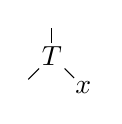
\begin{tikzpicture}[baseline=(T.base), inner sep=1pt]
      \node (T) {$T$};
      \node (x) at (.4,-.4) {$x$};
      \draw (T) -- (x);
      \draw (T) -- ++(-.3,-.3);
      \draw (T) -- ++(0,.35);
   \end{tikzpicture}
   \quad
   \text{and}
   \quad
   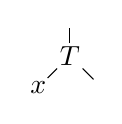
\begin{tikzpicture}[baseline=(T.base), inner sep=1pt]
      \node (T) {$T$};
      \node (x) at (-.4,-.4) {$x$};
      \draw (T) -- (x);
      \draw (T) -- ++(.3,-.3);
      \draw (T) -- ++(0,.35);
   \end{tikzpicture}
   \quad
   \text{and}
   \quad
   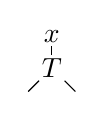
\begin{tikzpicture}[baseline=(T.base), inner sep=1pt]
      \node (T) {$T$};
      \node (x) at (0,.4) {$x$};
      \draw (T) -- (x);
      \draw (T) -- ++(.3,-.3);
      \draw (T) -- ++(-.3,-.3);
   \end{tikzpicture}
\]
To be perfectly precise about what each one means, we should give the edges labels.
For example we would write
$
   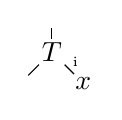
\begin{tikzpicture}[baseline=(T.base), inner sep=1pt]
      \node (T) {$T$};
      \node (x) at (.4,-.4) {$x$};
      \draw (T) -- (x) node[midway, above right, font=\tiny] {i};
      \draw (T) -- ++(-.3,-.3);
      \draw (T) -- ++(0,.3);
   \end{tikzpicture}
$
to specify the matrix $\sum_i T_i x_i$.
However, often the edge in question will be clear from the context, which is part of
what makes tensor diagram notation cleaner than, say, Einstein sum notation.

\[
   Y_{i,j} = \sum_{k,l,m,n,o} A_{i,k} B_{l,n,o} C_{j,k,l,m} D_{m,n} E_o
   \quad
   \Leftrightarrow
   % \quad
   \vcenter{\hbox{
      \import{figures/}{basic_graph.pdf_tex}
   }}
\]

The \emph{key principle} of tensor diagrams is that \emph{edge contraction is associative}.
This means you can contract any edge in any order you prefer.
This can be seen from the sum representation above, which can be reordered to sum over $k,l,m,n$ in any order.

The computational price for different contraction orders can be widely different.
Unfortunately it's not computationally easy to find the optimal order.
See section~\ref{sec:opt_contr} for algorithms to find the best contraction order, and approximate contraction methods.

Note that tensor graphs are not always connected.
We already saw that the outer product of two vectors can be written
   $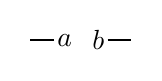
\begin{tikzpicture}[baseline=(a0.base), inner sep=1pt]
      \node (a0) {$a$};
      \node[right=.5em of a0] (a1) {$b$};
      \draw (a0.west) -- ++(-.3,0) node {};
      \draw (a1.east) -- ++(.3,0) node {};
   \end{tikzpicture}$.
This is natural from the sum representation: No edges simply means no sums.
So here $y_{i,j} = a_i b_j$, which is exactly the outer product $y=a\otimes b$.
% Can also mention how this gives us scaling by letter (5) be the order-0 tensor with value 5.


\section{The Copy Tensor}

A particularly important tensor is the ``copy'' tensor, also known as the ``diagonal'', ``kronecker delta'' or ``spider'' tensor.
The simplest version is the all-ones vector, which we write as $\sbullet-$.
That is $\sbullet_i = 1$.
The general order-n tensor is 1 on the diagonal, 0 everywhere else:
\[
   \sbullet_{i,j,k,\ldots} = \begin{cases}
      1\quad \text{if } i=j=k=\dots \\
      0\quad \text {otherwise}
   \end{cases}
\]
% This is also known as the ``copy'' or ``spider'' tensor, or ``generalized Kronecker delta''.
Or, using Iversonian notation, $\sbullet_{i,j,k,\dots} = [i=j=k=\dots]$.
We see the order-2 copy-tensor, $-\sbullet- = I$, is just the identity matrix,
so we can simply remove it from graphs like this:
\[-A\!-\!\sbullet\!-\!B- = -A\!-\!B-\]

Higher order copy-tensors are very useful, because they let us turn the simple tensor graphs into hyper-graphs.
A simple example of how we can use this is the diagonal matrix $D_a$, which has $a$ on the diagonal and 0 elsewhere.
We can write this as
\[
   D_a = 
   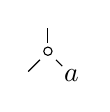
\begin{tikzpicture}[baseline=(T.base), inner sep=1pt]
      \node (T) {$\sbullet$};
      \node (x) at (.3,-.3) {$a$};
      \draw (T) -- (x);
      \draw (T) -- ++(-.25,-.25);
      \draw (T) -- ++(0,.3);
   \end{tikzpicture}
\]
Why?
Because $(D_a)_{i,j} = \sum_k \sbullet_{i,j,k} a_k = \sum_k [i=j=k] a_k = [i=j] a_i$.
Similarly the Hadamard product, $(a\circ b)_i = a_i b_i$, can be written
\[
   a \circ b =
   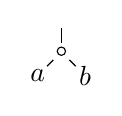
\begin{tikzpicture}[baseline=(T.base), inner sep=1pt]
      \node (T) {$\sbullet$};
      \node (a) at (-.3,-.3) {$a$};
      \node (b) at (.3,-.3) {$b$};
      \draw (T) -- (a);
      \draw (T) -- (b);
      \draw (T) -- ++(0,.3);
   \end{tikzpicture}
\]
Now, let's see why everyone loves copy tensors by using it to
prove the identity $D_aD_b = D_{a\circ b}$ by ``copy tensor manipulation'':
\[
   D_a D_b =
   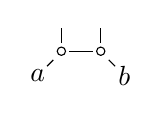
\begin{tikzpicture}[baseline=(T.base), inner sep=1pt]
      \node (T) {$\sbullet$};
      \node (a) at (-.3,-.3) {$a$};
      \draw (T) -- (a);
      \node (T2) at (.5,0) {$\sbullet$};
      \node (b) at (.8,-.3) {$b$};
      \draw (T) -- ++(0,.3);
      \draw (T) -- (T2);
      \draw (T2) -- (b);
      \draw (T2) -- ++(0,.3);
   \end{tikzpicture}
   =
   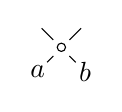
\begin{tikzpicture}[baseline=(T.base), inner sep=1pt]
      \node (T) {$\sbullet$};
      \node (a) at (-.3,-.3) {$a$};
      \node (b) at (.3,-.3) {$b$};
      \draw (T) -- (a);
      \draw (T) -- (b);
      \draw (T) -- ++(.25,.25);
      \draw (T) -- ++(-.25,.25);
   \end{tikzpicture}
   =
   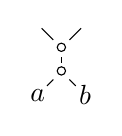
\begin{tikzpicture}[baseline=(T.base), inner sep=1pt]
      \node (T) {$\sbullet$};
      \node (a) at (-.3,-.3) {$a$};
      \node (b) at (.3,-.3) {$b$};
      \draw (T) -- (a);
      \draw (T) -- (b);
      \node (T2) at (0,.3) {$\sbullet$};
      \draw (T) -- (T2);
      \draw (T2) -- ++(.25,.25);
      \draw (T2) -- ++(-.25,.25);
   \end{tikzpicture}
   =
   D_{a\circ b}.
\]
You can verify this using the sum representation.

The general rule at play is that any connected sub-graph of copy-tensors can be combined into a single one.
Sometimes we are even lucky enough that this simplification leaves us with an identity matrix we can remove too:
%\begin{figure}[h]
%   \centering{
   %\def\svgwidth{.5\linewidth}
   %\import{figures/}{path1.pdf_tex}
   %\\
\[
   \def\svgwidth{.75\linewidth}
   \import{figures/}{path2.pdf_tex}
   .
\]
%   \caption{Contracting copy tensors and identity matrices}
%   \label{fig:spiders}
%   }
%\end{figure}
The only time you have to be a bit careful is when the resulting tensor has order 0.
Depending on how you define the order-0 copy tensor, $\sbullet$, you may or may not have the identity $\sbullet\!-\!\sbullet = \sbullet$.

Lots of other constructions that require special notation (like diagonal matrices or Hadamard products) with normal vector notation can be unified using the copy tensor.
%
In the Matrix Cookbook they define the order-4 tensor $J$,
which satisfies $J_{i,j,k,l} = [i=k][j=l]$ and which we'd write as
$J=\vcenter{\hbox{
   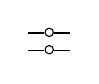
\begin{tikzpicture}[inner sep=0pt]
   \node (a0) {$\sbullet$};
   \draw (a0.east) -- ++(.2,0);
   \draw (a0.west) -- ++(-.2,0);
   \node[below=.2em of a0] (a1) {$\sbullet$};
   \draw (a1.east) -- ++(.2,0);
   \draw (a1.west) -- ++(-.2,0);
\end{tikzpicture}}}$,
and satisfies, for example, $\frac{dX}{dX}=J$.
Using ``tensor products'' you could write $J=I\otimes I$.
Note that $J$ is different from the order-4 copy-tensor,

\begin{tikzpicture}[baseline=(a0.base), inner sep=0pt]
   \node (a0) {$\sbullet$};
   \draw (a0) -- ++(.17,.17);
   \draw (a0) -- ++(.17,-.17);
   \draw (a0) -- ++(-.17,.17);
   \draw (a0) -- ++(-.17,-.17);
\end{tikzpicture}.

\section{Sums of Tensors}

Tensor products can express any linear function.
That is $f$ such that $f(a x, b y) = a b f(x,y)$.
Unfortunately not all operations on tensors are linear.
Even something as simple as a sum of two vectors, $x+y$, can not be displayed with a simple contraction graph.
(Note that this is not linear because $ax+by\neq ab(x+y)$.)

To handle this important operation, Penrose suggesting simply writing the two graphs with a plus sign between them, such as $-x + -y$.
Note that this is itself an order-1 tensor, even though it may look like there are two free edges.
If we want to multiply the sum with another tensor, we can use parentheses like $-M\!-\!(-x + -y)$.

It can be helpful to use named edges when dealing with sums, to make it clear how the edges are matched up.
Sums and tensor products interact nicely, with a general form of the distributive law:
%\begin{figure}[h]
%\centering{
%\def\svgwidth{\linewidth}
\[
\def\svgwidth{.75\linewidth}
\import{figures/}{path3.pdf_tex}
.
\]
%\caption{Distributive law}
%\label{fig:dist}
%}
%\end{figure}

When adding tensors that don't have the same number of edges, or have edges with different names, we can use ``broadcasting''.
%Say we want to add a matrix $\,_i\!-M-_j$ and a vector $x$.
Say we want to add a matrix $M$ and a vector $x$.
What does it even mean?
If we want to add $x$ to every row of $M$, we write
$
\vcenter{\hbox{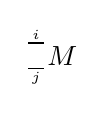
\begin{tikzpicture}[inner sep=1pt]
   \node (M) {$M$};
   \draw (M.north west) -- ++(-.2,0) node[midway, above, font=\tiny] {$i$};
   \draw (M.south west) -- ++(-.2,0) node[midway, below, font=\tiny] {$j$};
\end{tikzpicture}}}
+
\vcenter{\hbox{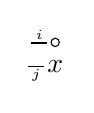
\begin{tikzpicture}[inner sep=1pt]
   \node (a0) {$\sbullet$};
   \draw (a0.west) -- ++(-.2,0) node[midway, above, font=\tiny] {$i$};
   \node[below=.2em of a0] (a1) {$x$};
   \draw (a1.west) -- ++(-.2,0) node[midway, below, font=\tiny] {$j$};
\end{tikzpicture}}}
$.
This is because
$
\vcenter{\hbox{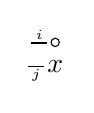
\begin{tikzpicture}[inner sep=1pt]
   \node (a0) {$\sbullet$};
   \draw (a0.west) -- ++(-.2,0) node[midway, above, font=\tiny] {$i$};
   \node[below=.2em of a0] (a1) {$x$};
   \draw (a1.west) -- ++(-.2,0) node[midway, below, font=\tiny] {$j$};
\end{tikzpicture}}}
$
is an outer product between $x$ and the all one vector, which is a matrix in which every row is the same.
Similarly, if we want to add $x$ to every column, we could use
the matrix
$
\vcenter{\hbox{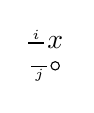
\begin{tikzpicture}[inner sep=1pt]
   \node (a0) {$\sbullet$};
   \draw (a0.west) -- ++(-.2,0) node[midway, below, font=\tiny] {$j$};
   \node[above=.2em of a0] (a1) {$x$};
   \draw (a1.west) -- ++(-.2,0) node[midway, above, font=\tiny] {$i$};
\end{tikzpicture}}}
$.

Note that we typically don't talk about ``rows'' or ``columns'' when dealing with tensors, but simply use the name edge (sometimes axis) of the tensor.
When using named edges, operations from classical vector notation like ``transpose'' can also be removed.
The matrix $X^T$ is simply $X$ where the left and right edge have been swapped.
But if the edges are named, we don't have to keep track on ``where the edge is'' at all.

\section{Transposition}
TODO: This section is not yet complete.

In classical matrix notation, transposition is denoted by a superscript T, as in $A^T$. This operation flips the indices of a matrix, so that $(A^T)_{ij} = A_{ji}$. In tensor diagram notation, we can represent transposition simply by swapping the positions of the edges:

\[
A^T = 
\begin{tikzpicture}[baseline=(A.base), inner sep=1pt]
   \node (A) {$A$};
   \draw (A.west) -- ++(-.3,0) node[left, font=\tiny] {$j$};
   \draw (A.east) -- ++(.3,0) node[right, font=\tiny] {$i$};
\end{tikzpicture}
\]

When using named edges, the concept of transposition becomes less relevant, as we can simply refer to the edges by their names regardless of their position. This allows for more flexible and intuitive manipulation of tensor expressions.

Let's examine some properties of transposition using tensor diagrams:

\begin{align*}
(A^T)^T &= A 
&
\begin{tikzpicture}[baseline=(A.base), inner sep=1pt]
   \node (A) {$A$};
   \draw (A.west) -- ++(-.3,0) node[left, font=\tiny] {$j$};
   \draw (A.east) -- ++(.3,0) node[right, font=\tiny] {$i$};
\end{tikzpicture}
&=
\begin{tikzpicture}[baseline=(A.base), inner sep=1pt]
   \node (A) {$A$};
   \draw (A.west) -- ++(-.3,0) node[left, font=\tiny] {$i$};
   \draw (A.east) -- ++(.3,0) node[right, font=\tiny] {$j$};
\end{tikzpicture}
\\
(AB)^T &= B^T A^T
&
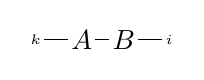
\begin{tikzpicture}[baseline=(A.base), inner sep=1pt]
   \node (A) {$A$};
   \node[right=.5em of A] (B) {$B$};
   \draw (A.west) -- ++(-.3,0) node[left, font=\tiny] {$k$};
   \path (A) edge (B);
   \draw (B.east) -- ++(.3,0) node[right, font=\tiny] {$i$};
\end{tikzpicture}^T
&=
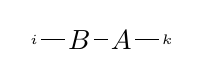
\begin{tikzpicture}[baseline=(B.base), inner sep=1pt]
   \node (B) {$B$};
   \node[right=.5em of B] (A) {$A$};
   \draw (B.west) -- ++(-.3,0) node[left, font=\tiny] {$i$};
   \path (B) edge (A);
   \draw (A.east) -- ++(.3,0) node[right, font=\tiny] {$k$};
\end{tikzpicture}
\\
(A + B)^T &= A^T + B^T
&
\left(
\begin{tikzpicture}[baseline=(A.base), inner sep=1pt]
   \node (A) {$A$};
   \draw (A.west) -- ++(-.3,0) node[left, font=\tiny] {$i$};
   \draw (A.east) -- ++(.3,0) node[right, font=\tiny] {$j$};
\end{tikzpicture}
+
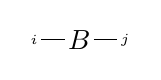
\begin{tikzpicture}[baseline=(B.base), inner sep=1pt]
   \node (B) {$B$};
   \draw (B.west) -- ++(-.3,0) node[left, font=\tiny] {$i$};
   \draw (B.east) -- ++(.3,0) node[right, font=\tiny] {$j$};
\end{tikzpicture}
\right)^T
&=
\begin{tikzpicture}[baseline=(A.base), inner sep=1pt]
   \node (A) {$A$};
   \draw (A.west) -- ++(-.3,0) node[left, font=\tiny] {$j$};
   \draw (A.east) -- ++(.3,0) node[right, font=\tiny] {$i$};
\end{tikzpicture}
+
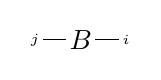
\begin{tikzpicture}[baseline=(B.base), inner sep=1pt]
   \node (B) {$B$};
   \draw (B.west) -- ++(-.3,0) node[left, font=\tiny] {$j$};
   \draw (B.east) -- ++(.3,0) node[right, font=\tiny] {$i$};
\end{tikzpicture}
\end{align*}

For higher-order tensors, transposition can be generalized to permutation of indices. For example, for a 3rd-order tensor $T_{ijk}$, we might consider $T_{jik}$ or $T_{kji}$. In tensor diagram notation, this simply corresponds to rearranging the edges:

\[
T_{ijk} = 
\begin{tikzpicture}[baseline=(T.base), inner sep=1pt]
   \node (T) {$T$};
   \draw (T) -- ++(.3,.3) node[above right, font=\tiny] {$i$};
   \draw (T) -- ++(-.3,.3) node[above left, font=\tiny] {$j$};
   \draw (T) -- ++(0,-.4) node[below, font=\tiny] {$k$};
\end{tikzpicture}
\qquad
T_{jik} = 
\begin{tikzpicture}[baseline=(T.base), inner sep=1pt]
   \node (T) {$T$};
   \draw (T) -- ++(.3,.3) node[above right, font=\tiny] {$j$};
   \draw (T) -- ++(-.3,.3) node[above left, font=\tiny] {$i$};
   \draw (T) -- ++(0,-.4) node[below, font=\tiny] {$k$};
\end{tikzpicture}
\qquad
T_{kji} = 
\begin{tikzpicture}[baseline=(T.base), inner sep=1pt]
   \node (T) {$T$};
   \draw (T) -- ++(.3,.3) node[above right, font=\tiny] {$k$};
   \draw (T) -- ++(-.3,.3) node[above left, font=\tiny] {$j$};
   \draw (T) -- ++(0,-.4) node[below, font=\tiny] {$i$};
\end{tikzpicture}
\]

This flexibility in representing transposition and index permutation is one of the advantages of tensor diagram notation, as it allows for clear visualization of these operations without the need for additional notation or symbols.

\section{Trace}

The ``trace'' of a square matrix is defined $\mathrm{Tr}(A) = \sum_i A_{i,i}$.
In tensor diagram notation, that corresponds to a self-edge: $\trace{A}{1}$.
The Matrix Cookbook has a list of identities using traces.
Let's reproduce them with tensor diagrams:
\begin{align*}
   \sum_{i=1}^{n} A_{ii} &= \mathrm{Tr}(A) = \mathrm{Tr}(A I)
   &
   \trace{A}{1} &= \trace{A, \sbullet}{2}
   \tag{11}
   \\%%%%%%%%%%%%%%%%%%%%%%%%%%%%%%%%%%%%%%%%
   \mathrm{Tr}(A) &= \mathrm{Tr}(A^T)
   &
   \trace{A}1 &= \trace{A}1
   \tag{13}
   \\%%%%%%%%%%%%%%%%%%%%%%%%%%%%%%%%%%%%%%%%
   \mathrm{Tr}(AB) &= \mathrm{Tr}(BA)
   &
   \trace{A,B}2 &= \trace{B,A}2
   \tag{14}
   \\%%%%%%%%%%%%%%%%%%%%%%%%%%%%%%%%%%%%%%%%
   \tag{15}
   \mathrm{Tr}(A+B)
   &= \mathrm{Tr}(A) + \mathrm{Tr}(B)
   &
   \trace{(A+B),\sbullet}1
   %\trace{(\matmul{A}+\matmul{B}),\sbullet}{2}
   &= \trace{A,\sbullet}2
 \\&&&+\trace{B,\sbullet}2
   \\%%%%%%%%%%%%%%%%%%%%%%%%%%%%%%%%%%%%%%%%
   \tag{16}
   \mathrm{Tr}(ABC) &= \mathrm{Tr}(BCA)
   &
   \trace{A,B,C}1 &= \trace{B,C,A}1
   \\
                  & = \mathrm{Tr}(CAB)
                  &&= \trace{C,A,B}1
   \\[0.5em]
   %%%%%%%%%%%%%%%%%%%%%%%%%%%%%%%%%%%%%%%%
   \tag{17}
   a^T a &= \mathrm{Tr}(a a^T)
   &
   \vecmatvec{1em}{a}{}{a}
   &=
   \mathrm{Tr}(
   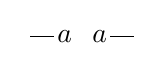
\begin{tikzpicture}[baseline=(a0.base), inner sep=1pt]
      \node (a0) {$a$};
      \node[right=.5em of a0] (a1) {$a$};
      \draw (a0.west) -- ++(-.3,0) node {};
      \draw (a1.east) -- ++(.3,0) node {};
   \end{tikzpicture}
   )
 \\&&&=
   \hspace{-1em}
   
\begin{tikzpicture}[baseline=(a0.base), inner sep=1pt]
      \node (a0) {$a$};
      \node[right=1em of a0] (a1) {$a$};
      \path (a0) edge [out=160, in=20, looseness=2] (a1);
   \end{tikzpicture}
   \hspace{-1em}
\end{align*}



\section{Eigenvalues}
Eigenvalues and eigenvectors are fundamental concepts in linear algebra that have important applications in tensor network theory. In tensor diagram notation, we can represent these concepts in a visually intuitive way.

For a matrix $A$, if there exists a non-zero vector $v$ and a scalar $\lambda$ such that $Av = \lambda v$, then $\lambda$ is called an eigenvalue of $A$, and $v$ is the corresponding eigenvector.
In tensor diagram notation It's convenient to write its eigendecomposition as $A = Q\Lambda Q^{-1}$, where $Q$ is a matrix whose columns are the eigenvectors of $A$, and $\Lambda$ is a diagonal matrix of the eigenvalues.
Thus:
\[
   \begin{tikzpicture}[baseline=(A.base), inner sep=1pt]
   \node (A) {$A$};
   \draw (A.west) -- ++(-.3, 0);
   \draw (A.east) -- ++(+.3, 0);
   \end{tikzpicture}
   =
   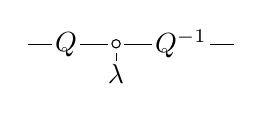
\begin{tikzpicture}[baseline=(Q.base), inner sep=1pt]
   \node (Q) {$Q$};
   \draw (Q.west) -- ++(-.3, 0);
   \node[right=1em of Q] (dot) {$\sbullet$};
   \path (Q) edge (dot);
   \node[below=.3em of dot] (e) {$\lambda$};
   \path (dot) edge (e);
   \node[right=1em of dot] (Qi) {$Q^{-1}$};
   \path (dot) edge (Qi);
   \draw (Qi.east) -- ++(.3, 0);
   \end{tikzpicture}
\]
The trace of a matrix is equal to the sum of its eigenvalues. We can represent this relationship using tensor diagrams:
\[
   \tag{12}
   \text{Tr}(A)
   =
   \hspace{-1em}
   \trace{A}{1}
   \hspace{-1em}
   =
   \hspace{-3em}
   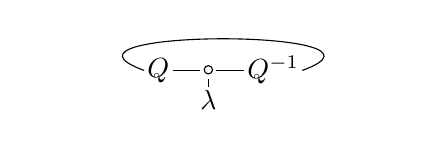
\begin{tikzpicture}[baseline=(Q.base), inner sep=1pt]
      \node (Q) {$Q$};
      \node[right=1em of Q] (dot) {$\sbullet$};
      \path (Q) edge (dot);
      \node[below=.3em of dot] (e) {$\lambda$};
      \path (dot) edge (e);
      \node[right=1em of dot] (Qi) {$Q^{-1}$};
      \path (dot) edge (Qi);
      \path (Q.west) edge [out=160, in=20, looseness=2] (Qi.east);
   \end{tikzpicture}
   \hspace{-3em}
   =
   \hspace{-1em}
   \begin{tikzpicture}[baseline=(dot.base), inner sep=1pt]
      \node (dot) {$\sbullet$};
      \node[below=.3em of dot] (e) {$\lambda$};
      \path (dot) edge (e);
      \path (dot) edge [out=160, in=20, loop] ();
   \end{tikzpicture}
   \hspace{-1em}
   =
   \begin{tikzpicture}[baseline=(dot.base), inner sep=1pt]
      \node (dot) {$\sbullet$};
      \node[below=.3em of dot] (e) {$\lambda$};
      \path (dot) edge (e);
   \end{tikzpicture}
   =
   \sum_i \lambda_i
\]



%\begin{enumerate}
   %\item Contractions are associative: You can contract edges in any order.
   %\item distributive law of sums/products.
   %\item Sums and broadcasting.
   %\item You can always contract connected subgraphs of Copy tensors.
%\end{enumerate}

\section{Exercises}
\begin{exercise}
   Given a sequence of matrices $A_1, A_2, \ldots, A_n \in \mathbb R^{n\times n}$,
   and vectors $v_1, v_2, \ldots, v_n \in \mathbb R^n$,
   draw, using tensor diagrams, the matrix made of vectors $A_1v_1, A_2v_2, \ldots, A_nv_n$.
\end{exercise}


\chapter{Simple Derivatives}

\section{Derivatives of Matrices, Vectors and Scalar Forms}

\subsection{First Order}

The Matrix Cookbook defines the single-entry matrix $J^{i,j} \in R^{n\times n}$ as the matrix which is zero everywhere except in the entry $(i, j)$ in which it is 1.
Alternatively we could write $J^{i,j}_{n,m} = [i=n][j=m]$.

\begin{align*}
   \tag{69}
   \frac{\partial x^T a}{\partial x}
   &= \frac{\partial a^T x}{\partial x}
   = a
   &
      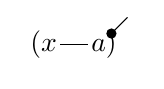
\begin{tikzpicture}[baseline=(a0.base), inner sep=1pt]
         \node (a0) {$(x$};
         \node[right=1em of a0] (a1) {$a)$};
         \path (a0) edge (a1);
         \draw [d] (a1.east) -- ++(.2,.2);
      \end{tikzpicture}
   &=
      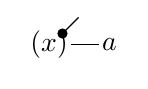
\begin{tikzpicture}[baseline=(a0.base), inner sep=1pt]
         \node (a0) {$(x)$};
         \node[right=1em of a0] (a1) {$a$};
         \path (a0) edge (a1);
         \draw [d] (a0.east) -- ++(.2,.2);
      \end{tikzpicture}
   =
      \begin{tikzpicture}[baseline=(a0.base), inner sep=1pt]
         \node (a0) {};
         \node[right=1em of a0] (a1) {$a$};
         \path (a0) edge (a1);
         \draw (a0.east) -- ++(-.1,-.2);
      \end{tikzpicture}
   \\
   %%%%%%%%%%%%%%%%%%%%%%%%%%%%%%%%%%%%%%%%
   \tag{70}
   \frac{\partial a^T X b}{\partial X} &= ab^T
   &
      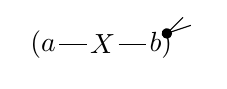
\begin{tikzpicture}[baseline=(a0.base), inner sep=1pt]
         \node (a0) {$(a$};
         \node[right=1em of a0] (a1) {$X$};
         \node[right=1em of a1] (a2) {$b)$};
         \path (a0) edge (a1);
         \path (a1) edge (a2);
         \draw[d] (a2.east) -- ++(.2,.2);
         \draw[d] (a2.east) -- ++(.3,.1);
      \end{tikzpicture}
   &=
      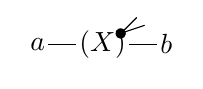
\begin{tikzpicture}[baseline=(a0.base), inner sep=1pt]
         \node (a0) {$a$};
         \node[right=1em of a0] (a1) {$(X)$};
         \node[right=1em of a1] (a2) {$b$};
         \path (a0) edge (a1);
         \path (a1) edge (a2);
         \draw[d] (a1.east) -- ++(.2,.2);
         \draw[d] (a1.east) -- ++(.3,.1);
      \end{tikzpicture}
      =
      \begin{tikzpicture}[baseline=(a0.base), inner sep=1pt]
         \node (a0) {$a$};
         \node[right=1em of a0] (a1) {};
         \node[right=1em of a1] (a2) {$b$};
         \path (a0) edge (a1);
         \path (a1) edge (a2);
         \draw (a1.west) -- ++(.1,.2);
         \draw (a1.east) -- ++(-.1,-.2);
      \end{tikzpicture}
   \\
   %%%%%%%%%%%%%%%%%%%%%%%%%%%%%%%%%%%%%%%%
   \tag{73}
   \frac{\partial X}{\partial X_{i,j}} &= J^{i,j}
   &
      \begin{tikzpicture}[baseline=(a0.base), inner sep=1pt]
         \node (a0) {$($};
         \node[right=1em of a0] (a1) {$X$};
         \node[right=1em of a1] (a2) {$)$};
         \path (a0) edge (a1);
         \path (a1) edge (a2);
         \draw[d] (a2.east) -- ++(.2,.2) node[midway, above left, font=\tiny] {i};
         \draw[d] (a2.east) -- ++(.3,.1) node[midway, below right, font=\tiny] {j};
      \end{tikzpicture}
   &=
      \begin{tikzpicture}[baseline=(a0.base), inner sep=1pt]
         \node (a0) {};
         \node[right=1em of a0] (a1) {};
         \node[right=1em of a1] (a2) {};
         \path (a0) edge (a1);
         \path (a1) edge (a2);
         \draw (a1.west) -- ++(.1,.2) node[midway, above left, font=\tiny] {i};
         \draw (a1.east) -- ++(-.1,-.2) node[midway, below right, font=\tiny] {j};
      \end{tikzpicture}
   \\
   %%%%%%%%%%%%%%%%%%%%%%%%%%%%%%%%%%%%%%%%
   \tag{74}
   \frac{\partial (X A)_{i,j}}{\partial X_{m,n}} &= (J^{m,n} A)_{i,j}
   &
      \begin{tikzpicture}[baseline=(a0.base), inner sep=1pt]
         \node (a0) {$($};
         \node[right=1em of a0] (a1) {$X$};
         \node[right=1em of a1] (a2) {$A$};
         \node[right=1em of a2] (a3) {$)$};
         \draw (a0) -- (a1) node[midway, above left, font=\tiny] {i};
         \draw (a1) -- (a2);
         \draw (a2) -- (a3) node[midway, below right, font=\tiny] {j};
         \draw[d] (a3.east) -- ++(.2,.2) node[midway, above left, font=\tiny] {m};
         \draw[d] (a3.east) -- ++(.3,.1) node[midway, below right, font=\tiny] {n};
      \end{tikzpicture}
   &=
      \begin{tikzpicture}[baseline=(a0.base), inner sep=1pt]
         \node (a0) {};
         \node[right=1em of a0] (a1) {$(X)$};
         \node[right=1em of a1] (a2) {$A$};
         \node[right=1em of a2] (a3) {};
         \path (a0) edge (a1);
         \path (a1) edge (a2);
         \path (a2) edge (a3);
         \draw[d] (a1.east) -- ++(.2,.2);
         \draw[d] (a1.east) -- ++(.3,.1);
      \end{tikzpicture}
 \\&&&=
      \begin{tikzpicture}[baseline=(a0.base), inner sep=1pt]
         \node (a0) {};
         \node[right=1em of a0] (a1) {};
         \node[right=1em of a1] (a2) {$A$};
         \node[right=1em of a2] (a3) {};
         \draw (a0) -- (a1) node[midway, above left, font=\tiny] {i};
         \draw (a1) -- (a2);
         \draw (a2) -- (a3) node[midway, below right, font=\tiny] {j};
         \draw (a1.west) -- ++(.1,.2) node[midway, above left, font=\tiny] {m};
         \draw (a1.east) -- ++(-.1,-.2) node[midway, below right, font=\tiny] {n};
      \end{tikzpicture}
\end{align*}

\subsection{Second Order}
\noindent
\makebox[\textwidth]{\parbox{1.1\textwidth}{%
\begin{align*}
   \tag{76}
   \frac{\partial}{\partial X_{i,j}}
   \sum_{k,l,m,n} X_{k,l} X_{m,n}
   &= (\sum_{k,l} X_{k,l})^2
   %&= \frac{\partial \|X\|_F^2}{\partial X_{i,j}}
   %&= 2\, \sum_{k,l} X_{k,l}
   &
   \begin{tikzpicture}[baseline=.5em, inner sep=1pt]
      \node (a0) at (0,0) {$\sbullet$};
      \node (a1) at (.5,0) {$X$};
      \node (a2) at (1,0) {$\sbullet$};
      \path (a0) edge (a1);
      \path (a1) edge (a2);
      \node (b0) at (0, .5) {$\sbullet$};
      \node (b1) at (.5, .5) {$X$};
      \node (b2) at (1, .5) {$\sbullet$};
      \path (b0) edge (b1);
      \path (b1) edge (b2);
      \node at (-.25, .25) {$\bigg($};
      \node at (1.25, .25) {$\bigg)$};
      \draw[d] (1.35, .4) -- ++(.2,.2) node[midway, above left, font=\tiny] {i};
      \draw[d] (1.35, .4) -- ++(.3,.1) node[midway, below right, font=\tiny] {j};
   \end{tikzpicture}
   &=
   \begin{tikzpicture}[baseline=.5em, inner sep=1pt]
      \node (a0) at (0,0) {$\sbullet$};
      \node (a1) at (.5,0) {$(X)$};
      \node (a2) at (1,0) {$\sbullet$};
      \path (a0) edge (a1);
      \path (a1) edge (a2);
      \node (b0) at (0, .5) {$\sbullet$};
      \node (b1) at (.5, .5) {$X$};
      \node (b2) at (1, .5) {$\sbullet$};
      \path (b0) edge (b1);
      \path (b1) edge (b2);
      \draw[d] (.83,.0) -- ++(.2,.2);
      \draw[d] (.83,.0) -- ++(.3,.1);
   \end{tikzpicture}
   +
   \begin{tikzpicture}[baseline=.5em, inner sep=1pt]
      \node (a0) at (0,0) {$\sbullet$};
      \node (a1) at (.5,0) {$X$};
      \node (a2) at (1,0) {$\sbullet$};
      \path (a0) edge (a1);
      \path (a1) edge (a2);
      \node (b0) at (0, .5) {$\sbullet$};
      \node (b1) at (.5, .5) {$(X)$};
      \node (b2) at (1, .5) {$\sbullet$};
      \path (b0) edge (b1);
      \path (b1) edge (b2);
      \draw[d] (0.83,.5) -- ++(.2,.2);
      \draw[d] (0.83,.5) -- ++(.3,.1);
   \end{tikzpicture}
   %\\[.3em]
   \\
   &= 2\, \sum_{k,l} X_{k,l}
   &&=
   2\,
   \begin{tikzpicture}[baseline=.5em, inner sep=1pt]
      \node (a0) at (0,0) {$\sbullet$};
      \node (a1) at (.5,0) {};
      \node (a2) at (1,0) {$\sbullet$};
      \path (a0) edge (a1);
      \path (a1) edge (a2);
      \node (b0) at (0, .5) {$\sbullet$};
      \node (b1) at (.5, .5) {$X$};
      \node (b2) at (1, .5) {$\sbullet$};
      \path (b0) edge (b1);
      \path (b1) edge (b2);
      \draw (a1.west) -- ++(.1,.2) node[midway, above left, font=\tiny] {i};
      \draw (a1.east) -- ++(-.1,-.2) node[midway, below right, font=\tiny] {j};
   \end{tikzpicture}
   %%%%%%%%%%%%%%%%%%%%%%%%%%%%%%%%%%%%%%%%
   \\[.5em]
   \tag{77} 
   \frac{\partial b^T X^T X c}{\partial X} &= X(bc^T + cb^T) 
   &
   \begin{tikzpicture}[baseline=(a0.base), inner sep=1pt]
      \node (a0) {$(\vecmatvec{.5em}{b}{X^T,X}{c})$};
      \draw[d] (a0.east) -- ++(.2,.2);
      \draw[d] (a0.east) -- ++(.3,.1);
   \end{tikzpicture}
   &=
   \begin{tikzpicture}[baseline=(a0.base), inner sep=1pt]
      \node (a0) {$b$};
      \node[right=1em of a0] (a1) {$X^T$};
      \node[right=1em of a1] (a2) {$(X)$};
      \node[right=1em of a2] (a3) {$c$};
      \draw (a0) -- (a1);
      \draw (a1) -- (a2);
      \draw (a2) -- (a3);
      \draw[d] (a2.east) -- ++(.2,.2);
      \draw[d] (a2.east) -- ++(.3,.1);
   \end{tikzpicture}
 \\&&&+
   \begin{tikzpicture}[baseline=(a0.base), inner sep=1pt]
      \node (a0) {$b$};
      \node[right=1em of a0] (a1) {$(X^T)$};
      \node[right=1em of a1] (a2) {$X$};
      \node[right=1em of a2] (a3) {$c$};
      \draw (a0) -- (a1);
      \draw (a1) -- (a2);
      \draw (a2) -- (a3);
      \draw[d] (a1.east) -- ++(.2,.2);
      \draw[d] (a1.east) -- ++(.3,.1);
   \end{tikzpicture}
   \\[.3em]&&&=
   \begin{tikzpicture}[baseline=(a0.base), inner sep=1pt]
      \node (a0) {$b$};
      \node[right=1em of a0] (a1) {$X^T$};
      \node[right=1em of a1] (a2) {};
      \node[right=1em of a2] (a3) {$c$};
      \draw (a0) -- (a1);
      \draw (a1) -- (a2);
      \draw (a2) -- (a3);
      \draw (a2.west) -- ++(.1,.2);
      \draw (a2.east) -- ++(-.1,-.2);
   \end{tikzpicture}
 \\&&&+
   \begin{tikzpicture}[baseline=(a0.base), inner sep=1pt]
      \node (a0) {$b$};
      \node[right=1em of a0] (a1) {};
      \node[right=1em of a1] (a2) {$X$};
      \node[right=1em of a2] (a3) {$c$};
      \draw (a0) -- (a1);
      \draw (a1) -- (a2);
      \draw (a2) -- (a3);
      \draw (a1.west) -- ++(.1,.2);
      \draw (a1.east) -- ++(-.1,-.2);
   \end{tikzpicture}
   \\[.3em]&&&=
   \begin{tikzpicture}[baseline=(a0.base), inner sep=1pt]
      \node (a0) {$X$};
      \node[right=.7em of a0] (a1) {$($};
      \node[right=.4em of a1] (a2) {$b\, c$};
      \node[right=.4em of a2] (a4) {$+$};
      \node[right=.6em of a4] (a5) {$c\, b$};
      \node[right=.2em of a5] (a7) {$)$};
      \draw (a0.west) -- ++(-.2,0);
      \draw (a0) -- (a1);
      \draw (a2.west) -- ++(-.2,0);
      \draw (a2.east) -- ++(.1,.15);
      \draw (a5.west) -- ++(-.2,0);
      \draw (a5.east) -- ++(.1,.15);
   \end{tikzpicture}
   \\
   \tag{78} 
   \frac{\partial}{\partial x} (Bx+b)^T C (Dx+d) &= B^TC(Dx+d)&&
                                \\&+D^TC^T(Bx+b) 
   &
   \dots &
   \\
   \tag{79} 
   \frac{\partial}{\partial X_{i,j}} (X^TBX)_{k,l} &= \delta_{l,j}(X^TB)_{k,i}
   %  \\&+ \delta_{k,j}(BX)_{i,l} 
   &
   \begin{tikzpicture}[baseline=(a0.base), inner sep=1pt]
      \node (a0) {$($};
      \node[right=.5em of a0] (a1) {$X^T$};
      \node[right=.5em of a1] (a2) {$B$};
      \node[right=.5em of a2] (a3) {$X$};
      \node[right=.5em of a3] (a4) {$)$};
      \draw (a0) -- (a1) node[midway, above left, font=\tiny] {k};
      \draw (a1) -- (a2);
      \draw (a2) -- (a3);
      \draw (a3) -- (a4) node[midway, below right, font=\tiny] {l};
      \draw[d] (a4.east) -- ++(.2,.2) node[midway, above left, font=\tiny] {i};
      \draw[d] (a4.east) -- ++(.3,.1) node[midway, below right, font=\tiny] {j};
   \end{tikzpicture}
   &=
   \begin{tikzpicture}[baseline=(a0.base), inner sep=1pt]
      \node (a0) {};
      \node[right=.5em of a0] (a1) {$X^T$};
      \node[right=.5em of a1] (a2) {$B$};
      \node[right=.5em of a2] (a3) {};
      \node[right=.5em of a3] (a4) {};
      \draw (a0) -- (a1) node[midway, above left, font=\tiny] {k};
      \draw (a1) -- (a2);
      \draw (a2) -- (a3);
      \draw (a3) -- (a4) node[midway, below right, font=\tiny] {l};
      \draw (a3.west) -- ++(.1,.2) node[midway, above left, font=\tiny] {i};
      \draw (a3.east) -- ++(-.1,-.2) node[midway, below right, font=\tiny] {j};
   \end{tikzpicture}
   \\
   &+ \delta_{k,j}(BX)_{i,l}
   &&+
   \begin{tikzpicture}[baseline=(a0.base), inner sep=1pt]
      \node (a0) {};
      \node[right=.5em of a0] (a1) {};
      \node[right=.5em of a1] (a2) {$B$};
      \node[right=.5em of a2] (a3) {$X$};
      \node[right=.5em of a3] (a4) {};
      \draw (a0) -- (a1) node[midway, above left, font=\tiny] {k};
      \draw (a1) -- (a2);
      \draw (a2) -- (a3);
      \draw (a3) -- (a4) node[midway, below right, font=\tiny] {l};
      \draw (a1.west) -- ++(.1,.2) node[midway, above left, font=\tiny] {j};
      \draw (a1.east) -- ++(-.1,-.2) node[midway, below right, font=\tiny] {i};
   \end{tikzpicture}
   %%%%%%%%%%%%%%%%%%%%%%%%%%%%%%%%%%%%%%%%
   \\
   \tag{80} 
   \frac{\partial}{\partial X_{i,j}} X^TBX &= X^TBJ^{i,j} + J^{j,i}BX 
   &
   \text{(same as above)} &
   %%%%%%%%%%%%%%%%%%%%%%%%%%%%%%%%%%%%%%%%
   \\
   \tag{81} 
   \frac{\partial}{\partial x} x^TBx &= (B+B^T)x 
   &
   \begin{tikzpicture}[baseline=(a0.base), inner sep=1pt]
      \node (a0) {$(x$};
      \node[right=.5em of a0] (a1) {$B$};
      \node[right=.5em of a1] (a2) {$x)$};
      \draw (a0) -- (a1);
      \draw (a1) -- (a2);
      \draw[d] (a2.east) -- ++(.2,.2) node[midway, above left, font=\tiny] {i};
      \draw[d] (a2.east) -- ++(.3,.1) node[midway, below right, font=\tiny] {j};
   \end{tikzpicture}
   &=
   \vecmatvec{.5em}{}{B}{x}
   + \vecmatvec{.5em}{x}{B}{}
 \\&&&=
   \begin{tikzpicture}[baseline=.5em, inner sep=1pt]
      \node (a0) at (0,0) {};
      \node (a1) at (.5,0) {$B$};
      \node (a2) at (1,0) {};
      \draw (a0) -- (a1) node[midway, below left, font=\tiny] {i};
      \draw (a1) -- (a2) node[midway, below right, font=\tiny] {j};
      \node (b0) at (0, .5) {};
      \node (b1) at (.5, .5) {$B$};
      \node (b2) at (1, .5) {};
      \draw (b0) -- (b1) node[midway, above left, font=\tiny] {j};
      \draw (b1) -- (b2) node[midway, above right, font=\tiny] {i};
      \node (l) at (-.3, .25) {$\bigg($};
      \node at (1.15, .25) {$\bigg)$};
      \node at (-.1, .25) {$+$};
      \node (x) at (-1,.25) {$x$};
      \draw (x) -- (l) node[midway, above right, font=\tiny] {i};
   \end{tikzpicture}
   %%%%%%%%%%%%%%%%%%%%%%%%%%%%%%%%%%%%%%%%
   \\
   \tag{82} 
   \frac{\partial}{\partial X} b^T X^T D X c &= D^T X b c^T + DXcb^T 
   &
   \dots &
   \\
   \tag{83} 
   \frac{\partial}{\partial X} (Xb+c)^T D (Xb+c) &= (D+D^T)(Xb+c)b^T 
   &
   \dots &
   \\
\end{align*}
}}

Assume $W$ is symmetric, then... (84) - (88)

\subsection{Higher-order and non-linear}


$$
\frac{\partial\left(\mathbf{X}^n\right)_{k l}}{\partial X_{i j}}=\sum_{r=0}^{n-1}\left(\mathbf{X}^r \mathbf{J}^{i j} \mathbf{X}^{n-1-r}\right)_{k l}
$$

For proof of the above, see B.1.3.
$$
\frac{\partial}{\partial \mathbf{X}} \mathbf{a}^T \mathbf{X}^n \mathbf{b}=\sum_{r=0}^{n-1}\left(\mathbf{X}^r\right)^T \mathbf{a b}^T\left(\mathbf{X}^{n-1-r}\right)^T
$$

\section{Derivatives of Traces}
Assume F(X) to be a differentiable function of each of the elements of X. It
then holds that
\[\frac{d \mathrm{Tr}(F(x))}{dX} = f(X)^T,\]
where $f(\cdot)$ is the scalar derivative of $F(\cdot)$.

TODO: To show this with tensor diagrams, we first need to introduce our notation for functions.

% Many more examples here: https://mbustamanter.github.io/ssg-blog/matder1/

\subsection{First Order}

\begin{align*}
   \tag{99}
   \frac{\partial}{\partial X} \mathrm{Tr}(X)
   &= I
   &
   \hspace{-1em}
   \begin{tikzpicture}[baseline=(a0.base), inner sep=1pt]
      \node (a0) {$($};
      \node[right=1em of a0] (a1) {$X$};
      \node[right=1em of a1] (a3) {$)$};
      \path (a1) edge[out=160, in=20, loop] (a1);
      \draw[d] (a3.east) -- ++(.2,.2);
      \draw[d] (a3.east) -- ++(.3,.1);
   \end{tikzpicture}
   \hspace{-1em}
   &=
   \hspace{-2em}
   \begin{tikzpicture}[baseline=(a0.base), inner sep=1pt]
      \node (a1) {$(X)$};
      \path (a1) edge[out=160, in=20, loop, looseness=4] (a1);
      \draw[d] (a1.south east) -- ++(.2,-.2);
      \draw[d] (a1.south east) -- ++(.3,-.1);
   \end{tikzpicture}
   \hspace{-2em}
 \\&&&=
   \hspace{-1.5em}
   \begin{tikzpicture}[baseline=(a0.base), inner sep=1pt]
      \node (a1) {$\phantom{X}$};
      \path (a1) edge[out=160, in=20, loop, looseness=6] (a1);
      \draw ($(a1.east)-(0,-.2em)$) -- ++(.2,-.1);
      \draw ($(a1.west)-(0,-.2em)$) -- ++(-.2,-.1);
   \end{tikzpicture}
   \hspace{-1.5em}
 \\&&&=
   \matmul{\sbullet}
   %%%%%%%%%%%%%%%%%%%%%%%%%%%%%%
   \\
   \tag{100}
   \frac{\partial}{\partial X} \mathrm{Tr}(XA)
   &= A^T
   &
   \begin{tikzpicture}[baseline=(a0.base), inner sep=1pt]
      \node (a0) {$($};
      \node[right=1em of a0] (a1) {$X$};
      \node[right=1em of a1] (a2) {$A$};
      \node[right=1em of a2] (a3) {$)$};
      \draw (a1) -- (a2);
      \path (a1) edge[out=160, in=20, looseness=2] (a2);
      \draw[d] (a3.east) -- ++(.2,.2);
      \draw[d] (a3.east) -- ++(.3,.1);
   \end{tikzpicture}
   &=
   \hspace{-2em}
   \begin{tikzpicture}[baseline=(a0.base), inner sep=1pt]
      \node (a1) {$(X)$};
      \node[right=1em of a1] (a2) {$A$};
      \draw (a1) -- (a2);
      \path (a1) edge[out=160, in=20, looseness=2] (a2);
      \draw[d] (a1.south east) -- ++(.2,-.2);
      \draw[d] (a1.south east) -- ++(.3,-.1);
   \end{tikzpicture}
   \hspace{-2em}
 \\&&&
   \hspace{-1.5em}
   \begin{tikzpicture}[baseline=(a0.base), inner sep=1pt]
      \node (a1) {$\phantom{X}$};
      \node[right=1em of a1] (a2) {$A$};
      \draw (a1) -- (a2);
      \path (a1) edge[out=160, in=20, looseness=2] (a2);
      \draw (a1.east) -- ++(.2,-.1);
      \draw ($(a1.west)-(0,-.2em)$) -- ++(-.2,-.1);
   \end{tikzpicture}
   \hspace{-1.5em}
 \\&&&
   = \matmul{A^T}
   %%%%%%%%%%%%%%%%%%%%%%%%%%%%%%
   \\
   \tag{101}
   \frac{\partial}{\partial X} \mathrm{Tr}(AXB)
   &= A^TB^T
   &
   \hspace{-1em}
   \begin{tikzpicture}[baseline=(a0.base), inner sep=1pt]
      \node (a0) {$($};
      \node[right=1em of a0] (a1) {$A$};
      \node[right=1em of a1] (a2) {$X$};
      \node[right=1em of a2] (a3) {$B$};
      \node[right=1em of a3] (a4) {$)$};
      \draw (a1) -- (a2) -- (a3);
      \path (a1) edge[out=160, in=20, looseness=2] (a3);
      \draw[d] (a4.east) -- ++(.2,.2);
      \draw[d] (a4.east) -- ++(.3,.1);
   \end{tikzpicture}
   \hspace{-1em}
   &=
   \hspace{-3em}
   \begin{tikzpicture}[baseline=(a0.base), inner sep=1pt]
      \node (a1) {$A$};
      \node[right=1em of a1] (a2) {$(X)$};
      \node[right=1em of a2] (a3) {$B$};
      \draw (a1) -- (a2) -- (a3);
      \path (a1) edge[out=160, in=20, looseness=2] (a3);
      \draw[d] (a2.south east) -- ++(.2,-.2);
      \draw[d] (a2.south east) -- ++(.3,-.1);
   \end{tikzpicture}
   \hspace{-3em}
 \\&&&=
   \hspace{-2.5em}
   \begin{tikzpicture}[baseline=(a0.base), inner sep=1pt]
      \node (a1) {$A$};
      \node[right=1em of a1] (a2) {$\phantom{X}$};
      \node[right=1em of a2] (a3) {$B$};
      \draw (a1) -- (a2) -- (a3);
      \path (a1) edge[out=160, in=20, looseness=2] (a3);
      \draw (a2.east) -- ++(.2,-.1);
      \draw (a2.west) -- ++(-.2,-.1);
   \end{tikzpicture}
   \hspace{-2.5em}
 \\&&&=
   \matmul{A^T, B^T}
\end{align*}


Continues for (102-105).
The last one uses the Kronecker product, which we may have to introduce first.

\subsection{Second Order}
\begin{align*}
   \frac{\partial}{\partial X} \mathrm{Tr}(X^2)
   &=2 X^T
   &
   \begin{tikzpicture}[baseline=(a0.base), inner sep=1pt]
      \node (a0) {$($};
      \node[right=1em of a0] (a1) {$X$};
      \node[right=1em of a1] (a2) {$X$};
      \node[right=1em of a2] (a3) {$)$};
      \draw (a1) -- (a2);
      \path (a1) edge[out=160, in=20, looseness=2] (a2);
      \draw[d] (a3.east) -- ++(.2,.2);
      \draw[d] (a3.east) -- ++(.3,.1);
   \end{tikzpicture}
   &=
   \hspace{-2em}
   \begin{tikzpicture}[baseline=(a0.base), inner sep=1pt]
      \node (a1) {$(X)$};
      \node[right=1em of a1] (a2) {$X$};
      \draw (a1) -- (a2);
      \path (a1) edge[out=160, in=20, looseness=2] (a2);
      \draw[d] (a1.south east) -- ++(.2,-.2);
      \draw[d] (a1.south east) -- ++(.3,-.1);
   \end{tikzpicture}
   \hspace{-2em}
   +
   \hspace{-2em}
   \begin{tikzpicture}[baseline=(a0.base), inner sep=1pt]
      \node (a1) {$X$};
      \node[right=1em of a1] (a2) {$(X)$};
      \draw (a1) -- (a2);
      \path (a1) edge[out=160, in=20, looseness=2] (a2);
      \draw[d] (a2.south east) -- ++(.2,-.2);
      \draw[d] (a2.south east) -- ++(.3,-.1);
   \end{tikzpicture}
   \hspace{-2em}
 \\&&&=
   \hspace{-1.5em}
   \begin{tikzpicture}[baseline=(a0.base), inner sep=1pt]
      \node (a1) {$\phantom{X}$};
      \node[right=1em of a1] (a2) {$X$};
      \draw (a1) -- (a2);
      \path (a1) edge[out=160, in=20, looseness=2] (a2);
      \draw (a1.east) -- ++(.2,-.1);
      \draw ($(a1.west)-(0,-.2em)$) -- ++(-.2,-.1);
   \end{tikzpicture}
   \hspace{-1.5em}
   +
   \hspace{-1.5em}
   \begin{tikzpicture}[baseline=(a0.base), inner sep=1pt]
      \node (a1) {$X$};
      \node[right=1em of a1] (a2) {$\phantom{X}$};
      \draw (a1) -- (a2);
      \path (a1) edge[out=160, in=20, looseness=2] (a2);
      \draw (a2.west) -- ++(-.2,-.1);
      \draw ($(a2.east)-(0,-.2em)$) -- ++(.2,-.1);
   \end{tikzpicture}
   \hspace{-1.5em}
 \\&&&=
   2\matmul{X^T}
\end{align*}
More:
\begin{align*}
& \frac{\partial}{\partial \mathbf{X}} \operatorname{Tr}\left(\mathbf{X}^2 \mathbf{B}\right)=(\mathbf{X B}+\mathbf{B X})^T \\
& \frac{\partial}{\partial \mathbf{X}} \operatorname{Tr}\left(\mathbf{X}^T \mathbf{B} \mathbf{X}\right)=\mathbf{B} \mathbf{X}+\mathbf{B}^T \mathbf{X} \\
& \frac{\partial}{\partial \mathbf{X}} \operatorname{Tr}\left(\mathbf{B} \mathbf{X} \mathbf{X}^T\right)=\mathbf{B} \mathbf{X}+\mathbf{B}^T \mathbf{X} \\
& \frac{\partial}{\partial \mathbf{X}} \operatorname{Tr}\left(\mathbf{X} \mathbf{X}^T \mathbf{B}\right)=\mathbf{B} \mathbf{X}+\mathbf{B}^T \mathbf{X} \\
& \frac{\partial}{\partial \mathbf{X}} \operatorname{Tr}\left(\mathbf{X B} \mathbf{X}^T\right)=\mathbf{X} \mathbf{B}^T+\mathbf{X B} \\
& \frac{\partial}{\partial \mathbf{X}} \operatorname{Tr}\left(\mathbf{B} \mathbf{X}^T \mathbf{X}\right)=\mathbf{X} \mathbf{B}^T+\mathbf{X B} \\
& \frac{\partial}{\partial \mathbf{X}} \operatorname{Tr}\left(\mathbf{X}^T \mathbf{X B}\right)=\mathbf{X} \mathbf{B}^T+\mathbf{X B} \\
& \frac{\partial}{\partial \mathbf{X}} \operatorname{Tr}(\mathbf{A X B X})=\mathbf{A}^T \mathbf{X}^T \mathbf{B}^T+\mathbf{B}^T \mathbf{X}^T \mathbf{A}^T \\
& \frac{\partial}{\partial \mathbf{X}} \operatorname{Tr}\left(\mathbf{X}^T \mathbf{X}\right)=\frac{\partial}{\partial \mathbf{X}} \operatorname{Tr}\left(\mathbf{X} \mathbf{X}^T\right)=2 \mathbf{X} \\
& \frac{\partial}{\partial \mathbf{X}} \operatorname{Tr}\left(\mathbf{B}^T \mathbf{X}^T \mathbf{C X B}\right)=\mathbf{C}^T \mathbf{X} \mathbf{B B}^T+\mathbf{C X B B}^T \\
& \frac{\partial}{\partial \mathbf{X}} \operatorname{Tr}\left[\mathbf{X}^T \mathbf{B X C}\right]=\mathbf{B X C}+\mathbf{B}^T \mathbf{X} \mathbf{C}^T \\
& \frac{\partial}{\partial \mathbf{X}} \operatorname{Tr}\left(\mathbf{A X B} \mathbf{X}^T \mathbf{C}\right)=\mathbf{A}^T \mathbf{C}^T \mathbf{X B}^T+\mathbf{C A X B} \\
& \frac{\partial}{\partial \mathbf{X}} \operatorname{Tr}\left[(\mathbf{A X B}+\mathbf{C})(\mathbf{A X B}+\mathbf{C})^T\right]=2 \mathbf{A}^T(\mathbf{A X B}+\mathbf{C}) \mathbf{B}^T \\
& \frac{\partial}{\partial \mathbf{X}} \operatorname{Tr}(\mathbf{X} \otimes \mathbf{X})=\frac{\partial}{\partial \mathbf{X}} \operatorname{Tr}(\mathbf{X}) \operatorname{Tr}(\mathbf{X})=2 \operatorname{Tr}(\mathbf{X}) \mathbf{I} \\
&
\end{align*}

\subsection{Higher Order}

\begin{align*}
\frac{\partial}{\partial \mathbf{X}} \operatorname{Tr}\left(\mathbf{X}^k\right)= & k\left(\mathbf{X}^{k-1}\right)^T \\
\frac{\partial}{\partial \mathbf{X}} \operatorname{Tr}\left(\mathbf{A} \mathbf{X}^k\right)= & \sum_{r=0}^{k-1}\left(\mathbf{X}^r \mathbf{A X}^{k-r-1}\right)^T \\
\frac{\partial}{\partial \mathbf{X}} \operatorname{Tr}\left[\mathbf{B}^T \mathbf{X}^T \mathbf{C X} \mathbf{X}^T \mathbf{C X B}\right]= & \mathbf{C X} \mathbf{X}^T \mathbf{C X B B}{ }^T \\
& +\mathbf{C}^T \mathbf{X B B} \mathbf{B}^T \mathbf{X}^T \mathbf{C}^T \mathbf{X} \\
& +\mathbf{C X B B}^T \mathbf{X}^T \mathbf{C X} \\
& +\mathbf{C}^T \mathbf{X X}^T \mathbf{C}^T \mathbf{X} \mathbf{B B}
\end{align*}

\subsection{Other}
$$
\frac{\partial}{\partial \mathbf{X}} \operatorname{Tr}\left(\mathbf{A} \mathbf{X}^{-1} \mathbf{B}\right)=-\left(\mathbf{X}^{-1} \mathbf{B} \mathbf{A} \mathbf{X}^{-1}\right)^T=-\mathbf{X}^{-T} \mathbf{A}^T \mathbf{B}^T \mathbf{X}^{-T}
$$

Assume $\mathbf{B}$ and $\mathbf{C}$ to be symmetric, then
$$
\begin{aligned}
\frac{\partial}{\partial \mathbf{X}} \operatorname{Tr}\left[\left(\mathbf{X}^T \mathbf{C X}\right)^{-1} \mathbf{A}\right] & =-\left(\mathbf{C X}\left(\mathbf{X}^T \mathbf{C X}\right)^{-1}\right)\left(\mathbf{A}+\mathbf{A}^T\right)\left(\mathbf{X}^T \mathbf{C X}\right)^{-1} \\
\frac{\partial}{\partial \mathbf{X}} \operatorname{Tr}\left[\left(\mathbf{X}^T \mathbf{C X}\right)^{-1}\left(\mathbf{X}^T \mathbf{B X}\right)\right] & =-2 \mathbf{C X}\left(\mathbf{X}^T \mathbf{C X}\right)^{-1} \mathbf{X}^T \mathbf{B X}\left(\mathbf{X}^T \mathbf{C X}\right)^{-1} \\
\frac{\partial}{\partial \mathbf{X}} \operatorname{Tr}\left[\left(\mathbf{A}+\mathbf{X}^T \mathbf{C X}\right)^{-1}\left(\mathbf{X}^T \mathbf{B X}\right)\right] & =-2 \mathbf{B X}\left(\mathbf{X}^T \mathbf{C X}\right)^{-1} \\
& -2 \mathbf{C X}\left(\mathbf{A}+\mathbf{X}^T \mathbf{C X}\right)^{-1} \mathbf{X}^T \mathbf{B X}\left(\mathbf{A}+\mathbf{X}^T \mathbf{C X}\right)^{-1} \\
& +2 \mathbf{B X}\left(\mathbf{A}+\mathbf{X}^T \mathbf{C X}\right)^{-1}
\end{aligned}
$$

See $[7]$.
$$
\frac{\partial \operatorname{Tr}(\sin (\mathbf{X}))}{\partial \mathbf{X}}=\cos (\mathbf{X})^T
$$



\chapter{Statistics and Probability}
\section{Definition of Moments}
Let $x\in\mathbb R^{n}$ is a random variable.
We write $m = E[x]\in\mathbb R^n$ for the expectation and
$M=\mathrm{Var}[x] = E[(x-m)(x-m)^T]$ for the covariance (when these quantities are defined.)

In tensor diagrams, we will use square brackets:
\[
   \vecmatvec{1em}{}{}{m}
   =
\mathbin{\begin{tikzpicture}[baseline=(n0.base), inner sep=1pt]
   \node (n0) at (0,0) {$[$};
   \node [right=1em of n0] (n1) {$x]$};
   \draw (n0) -- (n1);
\end{tikzpicture}}
\quad\text{and}\quad
   \vecmatvec{1em}{}{M}{}
   =
\mathbin{\begin{tikzpicture}[baseline=(n0.base), inner sep=1pt]
   \node (n0) at (0,0) {$[$};
   \node [right=1em of n0] (n1) {$(x\ominus m)$};
   \node [right=.5em of n1] (n2) {$(x\ominus m)$};
   \node [right=1em of n2] (n3) {$]$};
   \draw (n0) -- (n1);
   \draw (n2) -- (n3);
\end{tikzpicture}}
\]
We will use the circled minus, $\ominus$, to distinguish the operation from contraction edges.

We can also define the third and fourth centralized moment tensors
\[
   \begin{tikzpicture}[baseline=(T.base), inner sep=1pt]
      \node (T) {$M_3$};
      \draw (T) -- ++(.5,.3);
      \draw (T) -- ++(.5,-.3);
      \draw (T) -- ++(.5,0);
   \end{tikzpicture}
   =
   \renewcommand*{\arraystretch}{1.3}
   \begin{bmatrix}
      \vecmatvec{1em}{(x\ominus m)}{}{} \\
      \vecmatvec{1em}{(x\ominus m)}{}{} \\
      \vecmatvec{1em}{(x\ominus m)}{}{}
   \end{bmatrix}
\quad\text{and}\quad
   \begin{tikzpicture}[baseline=(T.base), inner sep=1pt]
      \node (T) {$M_4$};
      \draw (T) -- ++(.5,.5);
      \draw (T) -- ++(.5,-.5);
      \draw (T) -- ++(.5,.2);
      \draw (T) -- ++(.5,-.2);
   \end{tikzpicture}
   =
   \renewcommand*{\arraystretch}{1.3}
   \begin{bmatrix}
      \vecmatvec{1em}{(x\ominus m)}{}{} \\
      \vecmatvec{1em}{(x\ominus m)}{}{} \\
      \vecmatvec{1em}{(x\ominus m)}{}{} \\
      \vecmatvec{1em}{(x\ominus m)}{}{}
   \end{bmatrix}
.
\]
%These are less common in introductory causes, even though the scalar third and fourth moment are common.
%This is presumably because they require higher order tensors.

%If the entries of $x$ are independent, the non-diagonal entries disappear, so we get
%\[
%M =
%\left[
%   \begin{tikzpicture}[baseline=(c.base), inner sep=1pt]
%      \node (T1) {$(x\ominus m)$};
%      \node (T2)[below=.5em of T1] {$(x\ominus m)$};
%      \node (c)[right=.7em of T1, yshift=-1em] {$\sbullet$};
%      \draw (T1) -- (c);
%      \draw (T2) -- (c);
%      \draw (c) -- ++(.7em,0);
%   \end{tikzpicture}
%\right]
%\quad\text{and}\quad
%M_3 =
%\left[
%   \begin{tikzpicture}[baseline=(T2.base), inner sep=1pt]
%      \node (T1) {$(x\ominus m)$};
%      \node (T2)[below=.5em of T1] {$(x\ominus m)$};
%      \node (T3)[below=.5em of T2] {$(x\ominus m)$};
%      \node (c)[right=.7em of T2] {$\sbullet$};
%      \draw (T1) -- (c);
%      \draw (T2) -- (c);
%      \draw (T3) -- (c);
%      \draw (c) -- ++(.7em,0);
%   \end{tikzpicture}
%\right]
%\quad\text{and so on.}
%\]
% If the entries are also identically distributed, we simply have
% \[
%    M = \sigma^2
%    \,
% \begin{tikzpicture}[baseline=(T.base), inner sep=0]
%    \node (T) {$\sbullet$};
%    \draw (T) -- ++(0,.3);
%    \draw (T) -- ++(0,-.3);
% \end{tikzpicture}
%    \text{ and }
%    M_3 = \mathrm{E}[(x_0-m_0)^3]
% \begin{tikzpicture}[baseline=(T.base), inner sep=0]
%    \node (T) {$\sbullet$};
%    \draw (T) -- ++(0,.3);
%    \draw (T) -- ++(-.2,-.3);
%    \draw (T) -- ++(.2,-.3);
% \end{tikzpicture}
% .
% \]


\subsection{Expectation of Linear Combinations}
General principle: The ``linearity of expectation'' lets you pull out all parts of the graph not involving $X$.
\[
   \vcenter{\hbox{
      \import{figures/}{linearityOfExpectation.pdf_tex}
   }}
\]
where $M_3$ is the expectation\footnote{FIXME: This is different from the notation just introduced above.}
\(
\left[
\begin{tikzpicture}[baseline=(T.base), inner sep=1pt]
   \node (T) {$x$};
   \draw (T) -- ++(0,.3);
   \draw (T) -- ++(-.1,-.3);
   \draw (T) -- ++(.1,-.3);
\end{tikzpicture}
\,
\begin{tikzpicture}[baseline=(T.base), inner sep=1pt]
   \node (T) {$x$};
   \draw (T) -- ++(0,.3);
   \draw (T) -- ++(-.1,-.3);
   \draw (T) -- ++(.1,-.3);
\end{tikzpicture}
\,
\begin{tikzpicture}[baseline=(T.base), inner sep=1pt]
   \node (T) {$x$};
   \draw (T) -- ++(0,.3);
   \draw (T) -- ++(-.1,-.3);
   \draw (T) -- ++(.1,-.3);
\end{tikzpicture}
\right]
\),
which is an order-9 tensor with no dependence on the constants $A$, $B$, $C$ and $D$.
In practice you would want to name the edges to keep track of what gets multiplied with what.

We can even use linearity of expectation to push the expectation inside an infinite sum of tensors, as in the following moment generating function, which relates all the $M_k$ tensors:
\begin{align*}
   \mathrm{E}(\mathrm{e}^{\langle x\ominus m, t\rangle})
   &= \sum_{k=0}^\infty \frac{1}{k!} \mathrm{E}[\langle x\ominus m, t\rangle^k]
    = \mathrm{E}\big[\sum_{k=0}^\infty \frac{1}{k!} \langle (x\ominus m)^{\otimes k}, t^{\otimes k}\rangle\big]
   = \sum_{k=0}^\infty \frac{1}{k!} \langle M_k, t^{\otimes k}\rangle
 \\&=
  % =
   1
   +
   \begin{tikzpicture}[baseline=.5em, inner sep=1]
      \node (T) {$m$};
      \draw (T) -- ++(0,.5) node[fill=white] {$t$};
   \end{tikzpicture}
   +
   \frac{1}{2}
   \begin{tikzpicture}[baseline=(T.base), inner sep=1]
      \node (T) {$M$};
      \draw (T) -- ++(0,.5) node[fill=white] {$t$};
      \draw (T) -- ++(0,-.5) node[fill=white] {$t$};
   \end{tikzpicture}
   +
   \frac{1}{6}
   \begin{tikzpicture}[baseline=(T.base), inner sep=1]
      \node (T) {$M_3$};
      \draw (T) -- ++(0,.5) node[fill=white] {$t$};
      \draw (T) -- ++(-.4,-.4) node[fill=white] {$t$};
      \draw (T) -- ++(.4,-.4) node[fill=white] {$t$};
   \end{tikzpicture}
   +
   \frac{1}{24}
   \begin{tikzpicture}[baseline=(T.base), inner sep=1]
      \node (T) {$M_4$};
      \draw (T) -- ++(-.4,-.4) node[fill=white] {$t$};
      \draw (T) -- ++(.4,-.4) node[fill=white] {$t$};
      \draw (T) -- ++(-.4,.4) node[fill=white] {$t$};
      \draw (T) -- ++(.4,.4) node[fill=white] {$t$};
   \end{tikzpicture}
   +
   \dots
\end{align*}

\subsection{Linear Forms}
The Matrix Cookbook gives the following simple expectation:
\begin{walign}
   \tag{312}
   \E[AXB+C] &= A \E[X] B + C
   &
   \renewcommand*{\arraystretch}{1.3}
   \begin{bmatrix}
      \matmul{A,X,B} \\+\, \matmul{C}
   \end{bmatrix}
   &=
   \renewcommand*{\arraystretch}{1.3}
   \begin{matrix}
      \matmul{A,[X],B} \\+\, \matmul{C}
   \end{matrix}
\end{walign}

\subsection{Quadratic Forms}
We often prefer to write expectations in terms of the simple centered moments, which we can do by pulling out the mean:
\renewcommand*{\arraystretch}{1}
\[
   \begin{bmatrix}
      x - \\
      x -
   \end{bmatrix}
   =
   \begin{bmatrix}
      (x\ominus m) - \\
      (x\ominus m) -
   \end{bmatrix}
   +
   \begin{array}{c}
      m - \\
      m -
   \end{array}
   =
   \begin{tikzpicture}[baseline=(T.base), inner sep=1pt]
      \node (T) {$M$};
      \draw (T) -- ++(.5,.25);
      \draw (T) -- ++(.5,-.25);
   \end{tikzpicture}
   +
   \begin{array}{c}
      m - \\
      m -
   \end{array}
\]
This makes it easy to handle the quadratic forms from the Matrix Cookbook:
\begin{walign}
   \tag{313}
   \mathrm{Var}[Ax] &= A \mathrm{Var}[x] A^T
   &
   \renewcommand*{\arraystretch}{1.3}
   \begin{bmatrix}
      \vecmatvec{.5em}{A}{}{x} \ominus [\vecmatvec{.5em}{A}{}{x}] \\
      \vecmatvec{.5em}{A}{}{x} \ominus [\vecmatvec{.5em}{A}{}{x}]
   \end{bmatrix}
   &=
   \renewcommand*{\arraystretch}{1.3}
   \begin{bmatrix}
      \vecmatvec{.5em}{A}{}{(x\ominus m)} \\
      \vecmatvec{.5em}{A}{}{(x\ominus m)}
   \end{bmatrix}
 \\&&&=
   \vcenter{\hbox{\begin{tikzpicture}[inner sep=1pt]
      \node (n1) at (0,-.25) {$\vecmatvec{1em}{A}{}{(x\ominus m)}$};
      \node (n2) at (0,.25) {$\vecmatvec{1em}{A}{}{(x\ominus m)}$};
      \node at (-.45, 0) {$\Bigg[$};
      \node at (1, 0) {$\Bigg]$};
   \end{tikzpicture}}}
 \\&&& =
   \vecmatvec{.5em}{}{A,M_2,A}{}
%%%%%%%%%%%%%%%%%%%%%%%%%%%%%%%%%%%%%%%%%%%%%%%%%%%%%%%%%%%%%%%%%%%%%%%%%%%%%%%%
   \\[.5em]
   \tag{318}
   \E[x^T A x]
   &= \mathrm{Tr}(A M) + m^T A m
   &
   [\vecmatvec{.5em}{x}{A}{x}]
   &=
   \left(
      \begin{bmatrix}
         (x\ominus m) - \\
         (x\ominus m) -
      \end{bmatrix}
      +
      \begin{array}{c}
         m - \\
         m -
      \end{array}
   \right)
   \begin{tikzpicture}[baseline=(A.base), inner sep=1pt]
      \node (A) {$A$};
      \draw (A) -- ++(-.5, .1);
      \draw (A) -- ++(-.5, -.1);
   \end{tikzpicture}
   \\
   &&&=
   \mathbin{\begin{tikzpicture}[baseline=(A.base), inner sep=1pt]
      \node (n1) at (0,-.25) {$(x\ominus m)$};
      \node (n2) at (0,.25) {$(x\ominus m)$};
      \node at (-.75, 0) {$\Bigg[$};
      \node at (.75, 0) {$\Bigg]$};
      \node (A) at (1, 0) {$A$};
      \draw (n1) -- (A);
      \draw (n2) -- (A);
   \end{tikzpicture}}
   +
   \begin{tikzpicture}[baseline=(A.base), inner sep=1pt]
      \node (A) {$A$};
      \node (m1) at (-.75, .2) {$m$};
      \node (m2) at (-.75, -.2) {$m$};
      \draw (m1) -- (A) -- (m2);
   \end{tikzpicture}
   \\
   &&&=
   \trace{M,A}2
   +
   \vecmatvec{.5em}{m}{A}{m}
   \\[.5em]
\end{walign}

\begin{align*}
   E[(A\mathbf{x} + a)(B\mathbf{x} + b)^T] &= AMB^T + (Am + a)(Bm + b)^T \tag{320} \\
   E[\mathbf{x}\mathbf{x}^T] &= M + mm^T \tag{321} \\
   E[\mathbf{x} a^T \mathbf{x}] &= (M + mm^T)a \tag{322} \\
   E[\mathbf{x}^T a\mathbf{x}^T] &= a^T(M + mm^T) \tag{323} \\
   E[(A\mathbf{x})(A\mathbf{x})^T] &= A(M + mm^T)A^T \tag{324} \\
   E[(\mathbf{x} + a)(\mathbf{x} + a)^T] &= M + (m + a)(m + a)^T \tag{325} \\
   E[(A\mathbf{x} + a)^T(B\mathbf{x} + b)] &= \text{Tr}(AMB^T) + (Am + a)^T(Bm + b) \tag{326} \\
   E[\mathbf{x}^T \mathbf{x}] &= \text{Tr}(M) + m^T m \tag{327} \\
   E[\mathbf{x}^T A\mathbf{x}] &= \text{Tr}(AM) + m^T Am \tag{328} \\
   E[(A\mathbf{x})^T(A\mathbf{x})] &= \text{Tr}(AMA^T) + (Am)^T(Am) \tag{329} \\
   E[(\mathbf{x} + a)^T(\mathbf{x} + a)] &= \text{Tr}(M) + (m + a)^T(m + a) \tag{330}
\end{align*}



\subsection{Cubic Forms}

\[
\begin{tikzpicture}[scale=1.3,
  every node/.style={inner sep=1pt, circle, draw, fill=white, thin},
  label/.style={draw=none, fill=none, text=black, font=\scriptsize},
  declare function={
    xgap=.8;  % Horizontal spacing between diagrams
  }]

  \drawPartitionAtAngle{(-1.6*xgap,0)}{3}{$\kappa_3$}{{{1,2,3}}}
  \drawPartitionAtAngle{(0,0)}{3}{$+\kappa_2\kappa_1\Big($}{{{1,2},{3}}}
  \drawPartitionAtAngle{(xgap,0)}{3}{$+$}{{{1,3},{2}}}
  \drawPartitionAtAngle{(2*xgap,0)}{3}{$+$}{{{2,3},{1}}}
  \drawPartitionAtAngle{(3.6*xgap,0)}{3}{$\Big)+\kappa_1^3$}{{{1},{2},{3}}}

\end{tikzpicture}
\]


When $x$ is a stochastic vector with mean vector $m$,
it can be convenient to expand the raw third moment in terms of the central moments:

\renewcommand*{\arraystretch}{1}
\begin{align*}
\begin{bmatrix}
   x - \\
   x - \\
   x -
\end{bmatrix}
&=
\begin{bmatrix}
   (x\ominus m) - \\
   (x\ominus m) - \\
   (x\ominus m) -
\end{bmatrix}
\vspace{-.5em}
+
3
\hspace{-.25em}
\begin{array}{l}
\begin{bmatrix}
   (x\ominus m) -
\end{bmatrix}\\[.1em]
\begin{bmatrix}
   m - \\
   m -
\end{bmatrix}
\end{array}
\hspace{-.5em}
+
3
\hspace{-.25em}
\begin{array}{l}
\begin{bmatrix}
   m -
\end{bmatrix}\\[.1em]
\begin{bmatrix}
   (x\ominus m) - \\
   (x\ominus m) -
\end{bmatrix}
\end{array}
\hspace{-.5em}
+
\hspace{-.5em}
\begin{array}{c}
\begin{bmatrix}
   m -
\end{bmatrix}\\[.1em]
\begin{bmatrix}
   m -
\end{bmatrix}\\[.1em]
\begin{bmatrix}
   m -
\end{bmatrix}
\end{array}
%
\\&=
\begin{tikzpicture}[baseline=(T.base), inner sep=1pt]
   \node (T) {$M_3$};
   \draw (T) -- ++(0,.4);
   \draw (T) -- ++(-.2,-.35);
   \draw (T) -- ++(.2,-.35);
\end{tikzpicture}
+
3
\hspace{-.25em}
\begin{array}{c}
   m - \\
   -M-
\end{array}
\hspace{-.5em}
+
\begin{array}{c}
   m - \\
   m - \\
   m -
\end{array}
\end{align*}
TODO: The edges from the $m,M$ term needs to be symmetrized.


But this is still a bit of a mess.
See also below on Cumulants.



Assume \(\mathbf{x}\) to be a stochastic vector with independent coordinates, mean \(m\),
covariance \(M\) and central moments \(v_3 = \mathbb{E}[(\mathbf{x} - m)^3]\). Then (see [7])
\begin{align*}
&\mathbb{E}[(A\mathbf{x} + a)(B\mathbf{x} + b)^T (C\mathbf{x} + c)]
\\&\quad=
A\,\mathrm{diag}(B^T C) v_3
\\&\quad+
(Am + a) \mathrm{Tr}(BMC^T)
\\&\quad+
AMC^T (Bm + b)
\\&\quad\,+
AMB^T (Cm + c)
\\&\quad+
(Am + a)(Bm + b)^T (Cm + c)
\\
  &\mathbb{E}[\mathbf{x} \mathbf{x}^T \mathbf{x}]
\\&\quad=
   v_3
\\&\quad+
   2 Mm
\\&\quad+
   (\text{Tr}(M) + m^T m) m
\end{align*}


\section{Cumulants}

Given a random vector $x\in\mathbb R^d$,
its $n$th Cumulant Tensor, $K_n\in\R^{d,\ldots,d}$ is defined by
\[
   \log \mathrm{E}(\mathrm{e}^{\langle t, x\rangle})
   = \sum_{n=1}^\infty \frac{1}{n!} \langle K_n, t^{\otimes n}\rangle
   =
   \begin{tikzpicture}[baseline=.5em, inner sep=1]
      \node (T) {$K_1$};
      \draw (T) -- ++(0,.5) node[fill=white] {$t$};
   \end{tikzpicture}
   +
   \frac{1}{2}
   \begin{tikzpicture}[baseline=(T.base), inner sep=1]
      \node (T) {$K_2$};
      \draw (T) -- ++(0,.5) node[fill=white] {$t$};
      \draw (T) -- ++(0,-.5) node[fill=white] {$t$};
   \end{tikzpicture}
   +
   \frac{1}{6}
   \begin{tikzpicture}[baseline=(T.base), inner sep=1]
      \node (T) {$K_3$};
      \draw (T) -- ++(0,.5) node[fill=white] {$t$};
      \draw (T) -- ++(-.4,-.4) node[fill=white] {$t$};
      \draw (T) -- ++(.4,-.4) node[fill=white] {$t$};
   \end{tikzpicture}
   +
   \dots
\]
The first couple of cumulants are similar to the central moments:
\[
   K_1 = m
   \quad\text{and}\quad
   K_2 = M
   \quad\text{and}\quad
   K_3 = M_3
   \quad\text{and}\quad
   K_4 = M_4
   - \begin{tikzpicture}[baseline=-.8em, inner sep=.5pt]
      \node (M1) {\scriptsize $M_2$};
      \node[below=.4em of M1] (M2) {\scriptsize $M_2$};
      \draw (M1) -- ++(.35,0);
      \draw (M2) -- ++(.35,0);
      \draw (M1) -- ++(-.35,0);
      \draw (M2) -- ++(-.35,0);
   \end{tikzpicture}
   - \begin{tikzpicture}[baseline=(M1.base), inner sep=.5pt]
      \node (M1) {\scriptsize $M_2$};
      \node[right=.05em of M1] (M2) {\scriptsize $M_2$};
      \draw (M1) -- ++(-.25,.25);
      \draw (M1) -- ++(-.25,-.25);
      \draw (M2) -- ++(.25,.25);
      \draw (M2) -- ++(.25,-.25);
   \end{tikzpicture}
   - \begin{tikzpicture}[baseline=(M1.base), inner sep=.5pt]
      \node (M1) {\scriptsize $M_2$};
      \node[right=.05em of M1, yshift=-2pt] (M2) {\scriptsize $M_2$};
      \draw (M1) -- ++(-.25,.25);
      \draw (M1) -- ++(+.7,-.25);
      \draw (M2) -- ++(-.7,-.25);
      \draw (M2) -- ++(.25,.25);
   \end{tikzpicture}
   .
\]
They have the nice property (which is easy to see from the definition) that they are additive for independent random variables:
$
   K_n(x + y) = K_n(x) + K_n(y).
$
This generalizes the standard property that the variance of the sum of independent random variables is the sum of the variances.

We can write the expectations of $x^{\otimes n}$ in terms of the cumulants:

\[
   \begin{bmatrix}
      \begin{tikzpicture}[
         baseline=(T.base),
         every node/.style={inner sep=1pt, circle, draw=none, fill=white},
       ]
       \draw (30:.2) node[label] {$x$} -- (30:.6);
       \draw (150:.2) node[label] {$x$} -- (150:.6);
       \draw (270:.2) node[label] {$x$} -- (270:.6);
      \end{tikzpicture}
   \end{bmatrix}
   =
   \begin{tikzpicture}[
      baseline=-1em,
     every node/.style={inner sep=1pt, circle, draw, fill=white, thin},
     label/.style={draw=none, fill=none, text=black, font=\scriptsize},
     declare function={
       xgap=1.8;  % Horizontal spacing between diagrams
     }]
     \drawPartitionAtAngle[k]{(-1*xgap,0)}{3}{}{{{1,2,3}}}
     \drawPartitionAtAngle[k]{(0,0)}{3}{$+$}{{{1,2},{3}}}
     \drawPartitionAtAngle[k]{(xgap,0)}{3}{$+$}{{{1,3},{2}}}
     \drawPartitionAtAngle[k]{(xgap*2,0)}{3}{$+$}{{{1},{2,3}}}
     \drawPartitionAtAngle[k]{(xgap*3,0)}{3}{$+$}{{{1},{2},{3}}}
   \end{tikzpicture}
   .
\]
In general the sum is over all the partitions of the set $\{1,\ldots,n\}$.

If the entries of $x$ are \emph{independent}, the off-diagonals of the cumulant tensors $K_1, K_2, \dots$ are zero.
This means 
%
Assume each $x_i$ has cumulants $\kappa_1, \kappa_2, \kappa_3, \kappa_4 \in \R$, then
\[
\begin{bmatrix}
   \begin{tikzpicture}[
      baseline=(T.base),
      every node/.style={inner sep=1pt, circle, draw=none, fill=white},
    ]
    \draw (30:.2) node[label] {$x$} -- (30:.5);
    \draw (120:.2) node[label] {$x$} -- (120:.5);
    \draw (210:.2) node[label] {$x$} -- (210:.5);
    \draw (300:.2) node[label] {$x$} -- (300:.5);
   \end{tikzpicture}
\end{bmatrix}
=
\begin{tikzpicture}[
  every node/.style={inner sep=1pt, circle, draw, fill=white, thin},
  label/.style={draw=none, fill=none, text=black, font=\scriptsize},
  declare function={
    xgap=1;  % Horizontal spacing between diagrams
    ygap=.6;  % Vertical spacing between rows
  },
  baseline=-1cm
  ]
  \pgfmathsetmacro{\outerRadius}{.3}
  \pgfmathsetmacro{\innerRadius}{.1}

  % Pattern {4} - 1 partition
  \drawPartitionAtAngle{(0,0)}{4}{$\kappa_4$}{{{1,2,3,4}}}

  % Pattern {3,1} - 4 partitions
  \drawPartitionAtAngle{(0,-ygap)}{4}{$+\kappa_3\kappa_1\Big($}{{{1,2,3},{4}}}
  \drawPartitionAtAngle{(xgap,-ygap)}{4}{$+$}{{{1,2,4},{3}}}
  \drawPartitionAtAngle{(2*xgap,-ygap)}{4}{$+$}{{{2},{1,3,4}}}
  \drawPartitionAtAngle{(3*xgap,-ygap)}{4}{$+$}{{{1},{2,3,4}}}
  \node[label] at (3.5*xgap,-ygap) {$\Big)$};

  % Pattern {2,2} - 3 partitions
  \drawPartitionAtAngle{(0,-2*ygap)}{4}{$+\kappa_2^2\Big($}{{{1,2},{3,4}}}
  \drawPartitionAtAngle{(xgap,-2*ygap)}{4}{$+$}{{{1,3},{2,4}}}
  \drawPartitionAtAngle{(2*xgap,-2*ygap)}{4}{$+$}{{{1,4},{2,3}}}
  \node[label] at (2.5*xgap,-2*ygap) {$\Big)$};

  % Pattern {2,1,1} - 6 partitions
  \drawPartitionAtAngle{(0,-3*ygap)}{4}{$+\kappa_2\kappa_1^2\Big($}{{{1,2},{3},{4}}}
  \drawPartitionAtAngle{(xgap,-3*ygap)}{4}{$+$}{{{1,3},{2},{4}}}
  \drawPartitionAtAngle{(2*xgap,-3*ygap)}{4}{$+$}{{{1,4},{2},{3}}}
  \drawPartitionAtAngle{(3*xgap,-3*ygap)}{4}{$+$}{{{1},{2,3},{4}}}
  \drawPartitionAtAngle{(4*xgap,-3*ygap)}{4}{$+$}{{{1},{3},{2,4}}}
  \drawPartitionAtAngle{(5*xgap,-3*ygap)}{4}{$+$}{{{1},{2},{3,4}}}
  \node[label] at (5.5*xgap,-3*ygap) {$\Big)$};

  % Pattern {1,1,1,1} - 1 partition
  \drawPartitionAtAngle{(0,-4*ygap)}{4}{$+\kappa_1^4$}{{{1},{2},{3},{4}}}

\end{tikzpicture}
\]

Note in particular, that if the mean, $\kappa_1$, is zero, only four terms survive.
%\(
%\begin{tikzpicture}[
%   baseline=4em,
%  every node/.style={inner sep=1pt, circle, draw, fill=white, thin},
%  label/.style={draw=none, fill=none, text=black, font=\scriptsize},
%  declare function={
%    xgap=1;  % Horizontal spacing between diagrams
%    ygap=.6;  % Vertical spacing between rows
%  },
%  baseline=-1cm
%  ]
%  \pgfmathsetmacro{\outerRadius}{.3}
%  \pgfmathsetmacro{\innerRadius}{.1}
%
%  \drawPartitionAtAngle{(-1.5*xgap,0)}{4}{$\kappa_4$}{{{1,2,3,4}}}
%  \drawPartitionAtAngle{(0,0)}{4}{$+\kappa_2^2\Big($}{{{1,2},{3,4}}}
%  \drawPartitionAtAngle{(xgap,0)}{4}{$+$}{{{1,3},{2,4}}}
%  \drawPartitionAtAngle{(2*xgap,0)}{4}{$+$}{{{1,4},{2,3}}}
%  \node[label] at (2.5*xgap,0) {$\Big)$};
%\end{tikzpicture}
%.
%\)
For $n=5$ there are 52 partitions in total, but only 11 survive if $\kappa_1=0$:
\[
   \begin{tikzpicture}[
     every node/.style={inner sep=1pt, circle, draw, fill=white, thin},
     label/.style={draw=none, fill=none, text=black, font=\scriptsize},
     declare function={
       xgap=1;  % Horizontal spacing between diagrams
       ygap=.6;  % Vertical spacing between rows
     },
     baseline=-1cm
     ]
     \pgfmathsetmacro{\outerRadius}{.3}
     \pgfmathsetmacro{\innerRadius}{.1}
   % Pattern {5} - 1 partition
   \drawPartitionAtAngle{(-1.8*xgap,-ygap)}{5}{$\kappa_5$}{{{1,2,3,4,5}}}
   % Pattern {3,2} - 10 partitions
   \drawPartitionAtAngle{(0,-ygap)}{5}{$+\kappa_3\kappa_2\Big($}{{{1,2,3},{4,5}}}
   \drawPartitionAtAngle{(xgap,-ygap)}{5}{$+$}{{{3,5},{1,2,4}}}
   \drawPartitionAtAngle{(2*xgap,-ygap)}{5}{$+$}{{{1,2,5},{3,4}}}
   \drawPartitionAtAngle{(3*xgap,-ygap)}{5}{$+$}{{{1,3,4},{2,5}}}
   \drawPartitionAtAngle{(4*xgap,-ygap)}{5}{$+$}{{{1,3,5},{2,4}}}
   \drawPartitionAtAngle{(5*xgap,-ygap)}{5}{$+$}{{{1,4,5},{2,3}}}
   \drawPartitionAtAngle{(6*xgap,-ygap)}{5}{$+$}{{{1,5},{2,3,4}}}
   \drawPartitionAtAngle{(7*xgap,-ygap)}{5}{$+$}{{{2,3,5},{1,4}}}
   \drawPartitionAtAngle{(8*xgap,-ygap)}{5}{$+$}{{{1,3},{2,4,5}}}
   \drawPartitionAtAngle{(9*xgap,-ygap)}{5}{$+$}{{{1,2},{3,4,5}}}
   \node[label] at (9.5*xgap,-ygap) {$\Big)$};
   \end{tikzpicture}
\]

If $x$ is Gaussian, all cumulants of order $3$ and higher are zero.
For $n=6$ there are 203 partitions in total, but only 15 terms\footnote{This is why $\E[g^6]=15$ for $g\sim N(0,1)$.} for $E[x^{\otimes 6}]$:
\[
   \begin{tikzpicture}[
     every node/.style={inner sep=1pt, circle, draw, fill=white, thin},
     label/.style={draw=none, fill=none, text=black, font=\scriptsize},
     declare function={
       xgap=1;  % Horizontal spacing between diagrams
       ygap=.8;  % Vertical spacing between rows
     },
     baseline=-1cm
     ]
     \pgfmathsetmacro{\outerRadius}{.3}
     \pgfmathsetmacro{\innerRadius}{.1}
     % Pattern {2,2,2} - 15 partitions
     \drawPartitionAtAngle{(0,0)}{6}{$\kappa_2^3\Big($}{{{1,2},{3,4},{5,6}}}
     \drawPartitionAtAngle{(xgap,0)}{6}{$+$}{{{1,2},{3,5},{4,6}}}
     \drawPartitionAtAngle{(2*xgap,0)}{6}{$+$}{{{1,2},{3,6},{4,5}}}
     \drawPartitionAtAngle{(3*xgap,0)}{6}{$+$}{{{1,3},{2,4},{5,6}}}
     \drawPartitionAtAngle{(4*xgap,0)}{6}{$+$}{{{1,3},{2,5},{4,6}}}
     \drawPartitionAtAngle{(5*xgap,0)}{6}{$+$}{{{1,3},{2,6},{4,5}}}
     \drawPartitionAtAngle{(6*xgap,0)}{6}{$+$}{{{1,4},{2,3},{5,6}}}
     % row 2
     \drawPartitionAtAngle{(1*xgap,-ygap)}{6}{$+$}{{{1,4},{2,5},{3,6}}}
     \drawPartitionAtAngle{(2*xgap,-ygap)}{6}{$+$}{{{1,4},{2,6},{3,5}}}
     \drawPartitionAtAngle{(3*xgap,-ygap)}{6}{$+$}{{{1,5},{2,3},{4,6}}}
     \drawPartitionAtAngle{(4*xgap,-ygap)}{6}{$+$}{{{1,5},{2,4},{3,6}}}
     \drawPartitionAtAngle{(5*xgap,-ygap)}{6}{$+$}{{{1,5},{2,6},{3,4}}}
     \drawPartitionAtAngle{(6*xgap,-ygap)}{6}{$+$}{{{1,6},{2,3},{4,5}}}
     \drawPartitionAtAngle{(7*xgap,-ygap)}{6}{$+$}{{{1,6},{3,5},{2,4}}}
     \drawPartitionAtAngle{(8*xgap,-ygap)}{6}{$+$}{{{1,6},{3,4},{2,5}}}
     \node[label] at (8.5*xgap,-ygap) {$\Big)$};
     \end{tikzpicture}
     .
\]

\subsection{Quartic Forms}





We can use this to compute $\mathrm{Var}[x^T A x]$.
We assume $A$ is symmetric:
\begin{walign}
   \mathrm{Var}[x^T A x]
   &=
   \begin{tikzpicture}[baseline=.5em, inner sep=1pt, x=1.8em, y=1.2em]
      \node (x0) at (0,0) {$x$};
      \node (A0) at (1,0) {$A$};
      \node (x1) at (2,0) {$x$};
      \draw (x0) -- (A0) -- (x1);
      \node (x2) at (0,1) {$x$};
      \node (A1) at (1,1) {$A$};
      \node (x3) at (2,1) {$x$};
      \draw (x2) -- (A1) -- (x3);
      \draw (-.5,-.8) -- (2.5,-.8) -- (2.5,1.8) -- (1.5,1.8) -- (1.5,-.5) -- (.5,-.5) -- (.5,1.8) -- (-.5,1.8) -- (-.5,-.8);
   \end{tikzpicture}
   -
   \begin{tikzpicture}[baseline=.5em, inner sep=1pt, x=1.8em, y=1.2em]
      \node (x0) at (0,0) {$x$};
      \node (A0) at (1,0) {$A$};
      \node (x1) at (2,0) {$x$};
      \draw (x0) -- (A0) -- (x1);
      \node (x2) at (0,1) {$x$};
      \node (A1) at (1,1) {$A$};
      \node (x3) at (2,1) {$x$};
      \draw (x2) -- (A1) -- (x3);
      \draw (-.5,-.8) -- (2.5,-.8) -- (2.5,.4) -- (1.5,.4) -- (1.5,-.5) -- (.5,-.5) -- (.5,.4) -- (-.5,.4) -- (-.5,-.8);
      \draw (-.5,1.8) -- (2.5,1.8) -- (2.5,.6) -- (1.5,.6) -- (1.5,1.5) -- (.5,1.5) -- (.5,.6) -- (-.5,.6) -- (-.5,1.8);
   \end{tikzpicture}
   \\&=
   \kappa_4
   \begin{tikzpicture}[baseline=(A0.base), inner sep=0pt, fill=white]
       \node (A1) at (0,0) {$A$};
       \node (bullet) at (.8,0) {$\sbullet$};
       \node[anchor=west] (A2) at (1.4,0) {$A$};
       \draw (A1.east) to[out=45,in=135] (bullet) to[out=45,in=135] (A2.west);
       \draw (A1.east) to[out=-45,in=-135] (bullet) to[out=-45,in=-135] (A2.west);
   \end{tikzpicture}
   +
   4\kappa_3\kappa_1
   \begin{tikzpicture}[baseline=(A0.base), inner sep=1pt]
       \node (A1) at (0,0) {$A$};
       \node (bullet) at (.8,0) {$\sbullet$};
       \node[anchor=west] (A2) at (1.1,0) {$A$};
       \node (bullet2) at (1.8,0) {$\sbullet$};
       \draw (A1.east) to[out=45,in=135] (bullet) -- (A2.west);
       \draw (A1.east) to[out=-45,in=-135] (bullet);
       \draw (A2.east) -- (bullet2);
   \end{tikzpicture}
   \\&\quad+
   2 \kappa_2^2 \hspace{-.5em}\trace{A,A}{2}\hspace{-.5em} + \kappa_2^2 \hspace{-1em}\trace{A}{1}\hspace{-2em}\trace{A}{1}
   \\&\quad+
   4\kappa_2\kappa_1^2
   \begin{tikzpicture}[baseline=(A.base), inner sep=1pt]
       \node (bullet) at (0,0) {$\sbullet$};
       \node (A) at (.5,0) {$A$};
       \node (A2) at (1,0) {$A$};
       \node (bullet2) at (1.5,0) {$\sbullet$};
       \draw (bullet.east) -- (A.west);
       \draw (A.east) -- (A2.west);
       \draw (A2.east) -- (bullet2.west);
   \end{tikzpicture}
   +2\kappa_2\kappa_1^2
   \hspace{-1em} \trace{A}{1}\hspace{-1em}
   \vecmatvec{.5em}{\sbullet}{A}{\sbullet}
   \\&\quad+\kappa_1^4 \vecmatvec{.5em}{\sbullet}{A}{\sbullet}
   \vecmatvec{.5em}{\sbullet}{A}{\sbullet}
   \\&\quad-\big(
      \kappa_2 
      \hspace{-1em} \trace{A}{1}\hspace{-1em}
      +
      \kappa_1^2
      \vecmatvec{.5em}{\sbullet}{A}{\sbullet}
   \big)^2
   \\&=
   %%%
   2 \kappa_2^2 \hspace{-.5em}\trace{A,A}{2}\hspace{-.5em}
   +4\kappa_2\kappa_1^2
   \begin{tikzpicture}[baseline=(A.base), inner sep=1pt]
       \node (bullet) at (0,0) {$\sbullet$};
       \node (A) at (.5,0) {$A$};
       \node (A2) at (1,0) {$A$};
       \node (bullet2) at (1.5,0) {$\sbullet$};
       \draw (bullet.east) -- (A.west);
       \draw (A.east) -- (A2.west);
       \draw (A2.east) -- (bullet2.west);
   \end{tikzpicture}
   \\&\quad+
   4\kappa_3\kappa_1
   \begin{tikzpicture}[baseline=(A0.base), inner sep=1pt]
       \node (A1) at (0,0) {$A$};
       \node (bullet) at (.8,0) {$\sbullet$};
       \node[anchor=west] (A2) at (1.1,0) {$A$};
       \node (bullet2) at (1.8,0) {$\sbullet$};
       \draw (A1.east) to[out=45,in=135] (bullet) -- (A2.west);
       \draw (A1.east) to[out=-45,in=-135] (bullet);
       \draw (A2.east) -- (bullet2);
   \end{tikzpicture}
   +\kappa_4
   \begin{tikzpicture}[baseline=(A0.base), inner sep=0pt, fill=white]
       \node (A1) at (0,0) {$A$};
       \node (bullet) at (.8,0) {$\sbullet$};
       \node[anchor=west] (A2) at (1.4,0) {$A$};
       \draw (A1.east) to[out=45,in=135] (bullet) to[out=45,in=135] (A2.west);
       \draw (A1.east) to[out=-45,in=-135] (bullet) to[out=-45,in=-135] (A2.west);
   \end{tikzpicture}
\end{walign}
The Matrix Cookbook lists this as
\[
   \mathrm{Var}[x^T A x]
   =
   2\mu_2^2\text{Tr}(A^2)
   + 4\mu_2 c^T A^2 c
   + 4\mu_3 c^T Aa
   + (\mu_4 - 3\mu_2^2)a^T a \tag{319}
\]
where $c = \mu_1$ is the mean of $x$,
and $a = \mathrm{diag}(A)$ is the diagonal of $A$,
and $\mu_4 = \kappa_4 + 3\kappa_2^2$ is the fourth central moment.


\section{Weighted Scalar Variable}
Let $y=w^T x$, and let $m=E[y]$, then
\begin{align*}
   \tag{321}
   \E[y] &= m = w^T \mu
   \\
   \tag{322}
   \E[(y\ominus m)^2] &= \vecmatvec{.5em}{w}{M_2}{w}
   \\
   \tag{323}
   \E[(y\ominus m)^3] &=
   \mathbin{\begin{tikzpicture}[baseline=(a0.base), inner sep=1pt]
      \node (a0) {$M_3$};
      \node[above=.3em of a0] (n0) {$w$};
      \node[right=.3em of a0] (n1) {$w$};
      \node[left=.3em of a0] (n3) {$w$};
      \draw (a0.north) -- (n0);
      \draw (a0.east) -- (n1);
      \draw (a0.west) -- (n3);
   \end{tikzpicture}}
   \\
   \tag{324}
   \E[(y\ominus m)^4] &=
   \mathbin{\begin{tikzpicture}[baseline=(a0.base), inner sep=1pt]
      \node (a0) {$M_4$};
      \node[above=.3em of a0] (n0) {$w$};
      \node[right=.3em of a0] (n1) {$w$};
      \node[below=.3em of a0] (n2) {$w$};
      \node[left=.3em of a0] (n3) {$w$};
      \draw (a0.north) -- (n0);
      \draw (a0.east) -- (n1);
      \draw (a0.south) -- (n2);
      \draw (a0.west) -- (n3);
   \end{tikzpicture}}
\end{align*}


For $x\sim N(0,1)$, we have the inequality:
\[
   \E[y^n]^{1/n} \leq \sqrt{2/\pi}\, \|w\|_2.
\]


\section{Gaussian Moments}

For a Gaussian vector $x \sim \mathcal{N}(m,M)$:
- All odd centered moments vanish: $M_3 = 0$, etc.
- Even moments can be computed via Isserlis' theorem.

For instance:
\[
\mathbb{E}[(x \ominus m)^{\otimes 4}]
=
M \otimes M + M \otimes M + \dots
\]
(summing over the different pairings of indices).

\subsection{Gaussian Integration by Parts}
If $X$ is a tensor with Gaussian entries, zero mean, and some covariance,
% General principle for Gaussian expectations.
Stein's lemma gives the following very general equation, for any differentiable function $f$:
\[
   \vcenter{\hbox{
      \import{figures/}{steins.pdf_tex}
   }}
\]
Combined with the tensor chain rule from chapter~\ref{chapter:functions}, this can be a very powerful way to evaluate many hard expectations.



\begin{align*}
E(xx^T) &= \Sigma + mm^T \tag{377} \\
E[x^TAx] &= \text{Tr}(A\Sigma) + m^TAm \tag{378} \\
\text{Var}(x^TAx) &= \text{Tr}[A\Sigma(A + A^T)\Sigma] + \cdots \tag{379} \\
&\quad +m^T(A + A^T)\Sigma(A + A^T)m \\
E[(x - m')^TA(x - m')] &= (m - m')^TA(m - m') + \text{Tr}(A\Sigma) \tag{380}
\end{align*}

If $\Sigma = \sigma^2I$ and $A$ is symmetric, then

\begin{align*}
\text{Var}(x^TAx) = 2\sigma^4\text{Tr}(A^2) + 4\sigma^2m^TA^2m \tag{381}
\end{align*}

Assume $x \sim \mathcal{N}(0, \sigma^2I)$ and $A$ and $B$ to be symmetric, then

\begin{align*}
\text{Cov}(x^TAx, x^TBx) = 2\sigma^4\text{Tr}(AB) \tag{382}
\end{align*}

\subsection{Cubic forms}

Assume $x$ to be a stochastic vector with independent coordinates, mean $m$ and covariance $M$

\begin{align*}
E[xb^Txx^T] &= mb^T(M + mm^T) + (M + mm^T)bm^T \tag{383} \\
&\quad +b^Tm(M - mm^T)
\end{align*}

\subsection{Mean of Quartic Forms}

\begin{align*}
E[xx^Txx^T] &= 2(\Sigma + mm^T)^2 + m^Tm(\Sigma - mm^T) \\
&\quad +\text{Tr}(\Sigma)(\Sigma + mm^T) \\[1em]
E[xx^TAxx^T] &= (\Sigma + mm^T)(A + A^T)(\Sigma + mm^T) \\
&\quad +m^TAm(\Sigma - mm^T) + \text{Tr}[A\Sigma](\Sigma + mm^T) \\[1em]
E[x^Txx^Tx] &= 2\text{Tr}(\Sigma^2) + 4m^T\Sigma m + (\text{Tr}(\Sigma) + m^Tm)^2 \\[1em]
E[x^TAxx^TBx] &= \text{Tr}[A\Sigma(B + B^T)\Sigma] + m^T(A + A^T)\Sigma(B + B^T)m \\
&\quad +(\text{Tr}(A\Sigma) + m^TAm)(\text{Tr}(B\Sigma) + m^TBm)
\end{align*}

\begin{align*}
E[a^Txb^Txc^Txd^Tx] &= (a^T(\Sigma + mm^T)b)(c^T(\Sigma + mm^T)d) \\
&\quad +(a^T(\Sigma + mm^T)c)(b^T(\Sigma + mm^T)d) \\
&\quad +(a^T(\Sigma + mm^T)d)(b^T(\Sigma + mm^T)c) - 2a^Tmb^Tmc^Tmd^Tm
\end{align*}

\begin{align*}
&E[(Ax + a)(Bx + b)^T(Cx + c)(Dx + d)^T] \\
&= [A\Sigma B^T + (Am + a)(Bm + b)^T][C\Sigma D^T + (Cm + c)(Dm + d)^T] \\
&\quad +[A\Sigma C^T + (Am + a)(Cm + c)^T][B\Sigma D^T + (Bm + b)(Dm + d)^T] \\
&\quad +(Bm + b)^T(Cm + c)[A\Sigma D^T - (Am + a)(Dm + d)^T] \\
&\quad +\text{Tr}(B\Sigma C^T)[A\Sigma D^T + (Am + a)(Dm + d)^T]
\end{align*}

\begin{align*}
&E[(Ax + a)^T(Bx + b)(Cx + c)^T(Dx + d)] \\
&= \text{Tr}[A\Sigma(C^TD + D^TC)\Sigma B^T] \\
&\quad +[(Am + a)^TB + (Bm + b)^TA]\Sigma[C^T(Dm + d) + D^T(Cm + c)] \\
&\quad +[\text{Tr}(A\Sigma B^T) + (Am + a)^T(Bm + b)][\text{Tr}(C\Sigma D^T) + (Cm + c)^T(Dm + d)]
\end{align*}

See [7].


\subsection{Mixture of Gaussians}
For a mixture of Gaussians:
\[
   x \sim \sum_k \pi_k \mathcal{N}(m_k, M_k),
\]
the moments are weighted sums:
\[
   E[x] = \sum_k \pi_k m_k, \quad
   \mathrm{Var}[x] = \sum_k \pi_k (M_k + m_k m_k^T) - \left(\sum_k \pi_k m_k\right)\left(\sum_k \pi_k m_k\right)^T.
\]
Higher moments similarly combine via linearity.


\begin{align*}
E[x] &= \sum_k \rho_k m_k \tag{384} \\[1em]
\text{Cov}(x) &= \sum_k\sum_{k'} \rho_k\rho_{k'} (\Sigma_k + m_km_k^T - m_km_{k'}^T) \tag{385}
\end{align*}

\subsection{Derivatives}
Derivatives of moments with respect to $m$ or $M$ can be found by differentiating under the integral sign, and using Stein's lemma for Gaussian cases.

\section{Free Probability for Vectors and Tensors}

Free probability theory provides a non-commutative analogue of classical probability. We'll start with the simplest case—vectors with scalar entries—then progress to matrices and finally to higher-rank tensors.

\subsection{Free Cumulants for Vectors}

For a random vector $x \in \mathbb{R}^n$ with scalar entries, free cumulants are defined analogously to classical cumulants but using only non-crossing partitions.

\subsubsection{R-Transform for Vectors}

The R-transform (free cumulant generating function) is:
\[
   R_x(z) = \sum_{n=1}^{\infty} \kappa_n^{\text{free}} z^{n-1}
\]

This is the free analogue of the classical cumulant generating function $\log \mathrm{E}[e^{tz}] = \sum_{n=1}^{\infty} \frac{\kappa_n}{n!} t^n$.

\subsubsection{Moment-Cumulant Relations}

If each $x_i$ has free cumulants $\kappa_1^{\text{free}}, \kappa_2^{\text{free}}, \kappa_3^{\text{free}}, \kappa_4^{\text{free}} \in \mathbb{R}$, then:
\[
\begin{bmatrix}
   \begin{tikzpicture}[
      baseline=(T.base),
      every node/.style={inner sep=1pt, circle, draw=none, fill=white},
    ]
    \draw (30:.2) node[label] {$x$} -- (30:.5);
    \draw (120:.2) node[label] {$x$} -- (120:.5);
    \draw (210:.2) node[label] {$x$} -- (210:.5);
    \draw (300:.2) node[label] {$x$} -- (300:.5);
   \end{tikzpicture}
\end{bmatrix}_{\text{free}}
=
\begin{tikzpicture}[
  every node/.style={inner sep=1pt, circle, draw, fill=white, thin},
  label/.style={draw=none, fill=none, text=black, font=\scriptsize},
  crossing/.style={draw=red, fill=red!20},
  declare function={
    xgap=1;
    ygap=.6;
  },
  baseline=-1cm
  ]
  
  % Pattern {4} - 1 partition (non-crossing)
  \drawPartitionAtAngle{(0,0)}{4}{$\kappa_4^{\text{free}}$}{{{1,2,3,4}}}

  % Pattern {3,1} - 4 partitions total
  \drawPartitionAtAngle{(0,-ygap)}{4}{$+\kappa_3^{\text{free}}\kappa_1^{\text{free}}\Big($}{{{1,2,3},{4}}}
  \drawPartitionAtAngle[crossing]{(xgap,-ygap)}{4}{$\times$}{{{1,2,4},{3}}}
  \drawPartitionAtAngle[crossing]{(2*xgap,-ygap)}{4}{$\times$}{{{2},{1,3,4}}}
  \drawPartitionAtAngle{(3*xgap,-ygap)}{4}{$+$}{{{1},{2,3,4}}}
  \node[label] at (3.5*xgap,-ygap) {$\Big)$};

  % Pattern {2,2} - 3 partitions total
  \drawPartitionAtAngle{(0,-2*ygap)}{4}{$+(\kappa_2^{\text{free}})^2\Big($}{{{1,2},{3,4}}}
  \drawPartitionAtAngle[crossing]{(xgap,-2*ygap)}{4}{$\times$}{{{1,3},{2,4}}}
  \drawPartitionAtAngle{(2*xgap,-2*ygap)}{4}{$+$}{{{1,4},{2,3}}}
  \node[label] at (2.5*xgap,-2*ygap) {$\Big)$};

  % Pattern {2,1,1} - 6 partitions total
  \drawPartitionAtAngle{(0,-3*ygap)}{4}{$+\kappa_2^{\text{free}}(\kappa_1^{\text{free}})^2\Big($}{{{1,2},{3},{4}}}
  \drawPartitionAtAngle[crossing]{(xgap,-3*ygap)}{4}{$\times$}{{{1,3},{2},{4}}}
  \drawPartitionAtAngle[crossing]{(2*xgap,-3*ygap)}{4}{$\times$}{{{1,4},{2},{3}}}
  \drawPartitionAtAngle[crossing]{(3*xgap,-3*ygap)}{4}{$\times$}{{{1},{2,3},{4}}}
  \drawPartitionAtAngle[crossing]{(4*xgap,-3*ygap)}{4}{$\times$}{{{1},{3},{2,4}}}
  \drawPartitionAtAngle{(5*xgap,-3*ygap)}{4}{$+$}{{{1},{2},{3,4}}}
  \drawPartitionAtAngle{(6*xgap,-3*ygap)}{4}{$+$}{{{1,4},{2},{3}}}
  \node[label] at (6.5*xgap,-3*ygap) {$\Big)$};

  % Pattern {1,1,1,1} - 1 partition (non-crossing)
  \drawPartitionAtAngle{(0,-4*ygap)}{4}{$+(\kappa_1^{\text{free}})^4$}{{{1},{2},{3},{4}}}

  % Legend
  \node[label, red] at (4,-5*ygap) {\small Red = crossing partitions (excluded in free probability)};

\end{tikzpicture}
\]

Compare with classical: 15 partitions $\to$ 9 non-crossing partitions!

\subsection{Free Cumulants for Matrices}

For random matrices, we must consider traces of products. Unlike scalars, matrix products don't commute, adding complexity.
\[
\begin{tikzpicture}[baseline=-.5em, scale=0.8]
   % Classical vs Free
   \node at (-2,1) {\small Classical cumulants:};
   \node at (-2,-1.5) {\small Free cumulants:};
   
   % Classical - all 5 partitions
   \node at (0,1) {$\mathrm{E}[X^3] =$};
   \node at (2,1) {$\kappa_3$};
   \node at (3,1) {$+ 3\kappa_2\kappa_1$};
   \node at (5,1) {$+ \kappa_1^3$};
   \node at (7,1) {\small (5 partitions)};
   
   % Free - only 2 non-crossing
   \node at (0,-1.5) {$\mathrm{E}[\mathrm{Tr}(X^3)] =$};
   \node at (2.5,-1.5) {$\kappa_3^{\text{free}}$};
   \node at (4.5,-1.5) {$+ \kappa_1^{\text{free}}\kappa_2^{\text{free}}$};
   \node at (7,-1.5) {\small (2 NC partitions)};
\end{tikzpicture}
\]

The partition $(1,3),(2)$ is crossing and thus excluded in free probability:
\[
\begin{tikzpicture}[baseline=0, scale=0.7]
   % Non-crossing partitions
   \node at (-2,0) {\small Non-crossing:};
   \foreach \i in {1,2,3} {
      \node[circle, draw] (A\i) at (120-120*\i:1) {\tiny \i};
   }
   \draw[thick] (A1) to (A2);
   \draw[thick] (A3) to (A3);
   
   \begin{scope}[xshift=4cm]
      \foreach \i in {1,2,3} {
         \node[circle, draw] (B\i) at (120-120*\i:1) {\tiny \i};
      }
      \draw[thick] (B1) to (B1);
      \draw[thick] (B2) to (B3);
   \end{scope}
   
   % Crossing partition
   \begin{scope}[xshift=8cm]
      \node at (-2,0) {\small Crossing:};
      \foreach \i in {1,2,3} {
         \node[circle, draw] (C\i) at (120-120*\i:1) {\tiny \i};
      }
      \draw[thick, red] (C1) to (C3);
      \draw[thick] (C2) to (C2);
      \node[red] at (0,-2) {\small $\times$};
   \end{scope}
\end{tikzpicture}
\]

Key insight: For matrices, we have ONE edge to match between elements. For higher-rank tensors, we have MULTIPLE edges (colors) to match.

\subsection{Tensor Free Cumulants}

For rank-$D$ tensors, the free cumulant theory becomes richer due to colored non-crossing partitions.

\subsubsection{Colored Non-Crossing Partitions for Tensors}

For rank-$D$ tensors, each element has $D$ "legs" or indices. A valid pairing must:
\begin{itemize}
\item Be non-crossing when elements are arranged on a circle
\item Match ALL $D$ colors (one per leg) between paired elements
\end{itemize}

This dramatically reduces the number of valid partitions. For rank-3 tensors:
\[
\begin{tikzpicture}[baseline=-.5em, scale=0.8]
   % Matrix case
   \node at (-3,0) {\small Matrices:};
   \node[draw, thick] (M1) at (-1,0) {$X$};
   \node[draw, thick] (M2) at (0.5,0) {$X$};
   \draw[thick] (M1.east) -- (M2.west) node[midway, above] {\tiny 1 edge};
   
   % Tensor case
   \node at (2,0) {\small Rank-3 tensors:};
   \node[draw, thick] (T1) at (4,0) {$T$};
   \node[draw, thick] (T2) at (5.5,0) {$T$};
   % Must connect all 3 colors
   \draw[cyan, thick] (T1.north east) to[bend left=20] (T2.north west);
   \draw[magenta, thick] (T1.east) -- (T2.west);
   \draw[yellow, thick] (T1.south east) to[bend right=20] (T2.south west);
   \node at (7.5,0) {\tiny 3 edges};
\end{tikzpicture}
\]

\subsubsection{Invariant Traces for Tensors}

Unlike matrices, higher-rank tensors have no single canonical trace. Instead, every way of contracting tensors to produce a scalar defines a different invariant:

\begin{center}
\begin{tabular}{|l|l|}
\hline
Matrices ($D=2$) & Tensors ($D>2$) \\
\hline
Unique invariant $\mathrm{Tr}(X_1 \cdots X_n)$ & Family of invariants $\mathrm{Tr}_{\pi}(T_1,\ldots,T_n)$ \\
& indexed by colored permutations $\pi \in \mathfrak{S}_{Dn}$ \\
\hline
\end{tabular}
\end{center}

\textbf{Definition of $\mathrm{Tr}_{\pi}$:} Given tensors $T_1,\ldots,T_n$ each with $D$ legs (colored 1 through $D$), a colored permutation $\pi = (\pi^{(1)},\ldots,\pi^{(D)}) \in \mathfrak{S}_n^D$ specifies which legs connect:

\[
\mathrm{Tr}_{\pi}(T_1,\ldots,T_n) = 
\begin{tikzpicture}[baseline=0, scale=0.8]
   % Example for n=3, D=3
   \node at (-2,0) {\small Example:};
   % Three tensors
   \node[draw, thick] (T1) at (90:1.2) {$T_1$};
   \node[draw, thick] (T2) at (210:1.2) {$T_2$};
   \node[draw, thick] (T3) at (330:1.2) {$T_3$};
   
   % Permutation pi^(1) for cyan: (1 2 3)
   \draw[cyan, thick] (T1) to[bend right=30] node[midway, left] {\tiny $\pi^{(1)}$} (T2);
   \draw[cyan, thick] (T2) to[bend right=30] (T3);
   \draw[cyan, thick] (T3) to[bend right=30] (T1);
   
   % Permutation pi^(2) for magenta: (1 3 2)
   \draw[magenta, thick] (T1) to[bend left=20] node[midway, right] {\tiny $\pi^{(2)}$} (T3);
   \draw[magenta, thick] (T3) to[bend left=20] (T2);
   \draw[magenta, thick] (T2) to[bend left=20] (T1);
   
   % Permutation pi^(3) for yellow: (1)(2)(3)
   \draw[yellow, thick] (T1) to[out=60,in=120,looseness=8] (T1);
   \draw[yellow, thick] (T2) to[out=180,in=240,looseness=8] (T2);
   \draw[yellow, thick] (T3) to[out=300,in=360,looseness=8] (T3);
\end{tikzpicture}
\]

For matrices ($D=2$), only the cyclic permutation gives a non-zero trace, recovering the usual $\mathrm{Tr}(X_1 X_2 \cdots X_n)$.

\textbf{Normalization:} To obtain finite limits as $N \to \infty$, we normalize by $N^{-(D-1)n}$:
\[
   \frac{1}{N^{(D-1)n}} \mathrm{Tr}_{\pi}(T_1,\ldots,T_n) \xrightarrow{N \to \infty} \text{finite}
\]

\subsubsection{Moment-Cumulant Formula}

The tensor moment-cumulant relation involves ALL invariant traces:
\[
   \boxed{\left( \mathrm{E}[\mathrm{Tr}_{\pi}(T_{i_1},\ldots,T_{i_n})] \right)_{\pi \in \mathrm{NC}_D(n)} = \sum_{\sigma \in \mathrm{NC}_D(n)} \kappa_{\sigma}^{(\mathrm{t})} \cdot (\text{pattern matching})}
\]

The moments form a vector indexed by colored non-crossing permutations, and tensor freeness acts on this entire family.

Example for $n=2$: The second moment decomposes as
\[
\begin{tikzpicture}[baseline=-.5em, scale=0.8]
   % Moment
   \node at (-1,0) {$\mathrm{E}[\mathrm{Tr}(T_1 T_2)]$};
   \node at (1,0) {$=$};
   
   % First term: partition (1,2)
   \node at (2.5,0) {$\kappa_2^{(\mathrm{t})}$};
   \node[circle, draw, inner sep=1pt] (A1) at (3.5,0.3) {\tiny 1};
   \node[circle, draw, inner sep=1pt] (A2) at (3.5,-0.3) {\tiny 2};
   \draw[thick] (A1) -- (A2);
   \node at (4.2,0) {$\delta_{i_1,i_2}$};
   
   \node at (5.5,0) {$+$};
   
   % Second term: partition (1),(2)
   \node at (6.5,0) {$(\kappa_1^{(\mathrm{t})})^2$};
   \node[circle, draw, inner sep=1pt] (B1) at (7.5,0.3) {\tiny 1};
   \node[circle, draw, inner sep=1pt] (B2) at (7.5,-0.3) {\tiny 2};
\end{tikzpicture}
\]

For Gaussian tensors, $\kappa_1^{(\mathrm{t})} = 0$ and $\kappa_n^{(\mathrm{t})} = 0$ for $n > 2$, so:
\[
   \mathrm{E}[\mathrm{Tr}(T_1 T_2)] = \kappa_2^{(\mathrm{t})} \delta_{i_1,i_2} = \delta_{i_1,i_2}
\]

\subsection{Tensor Wick Theorem}

For Gaussian tensors, a fundamental result analogous to Wick's theorem holds:

Tensor Wick Factorization:
Let $(T_i)_{i \in I}$ be i.i.d. standard Gaussian $D$-leg tensors of size $N$. As $N \to \infty$:
\[
   \mathrm{E}[T_{i_1} \cdots T_{i_{2k}}] = \sum_{\pi \in \mathrm{NC}_D(2k)} \prod_{(j,j') \in \pi} \delta_{i_j, i_{j'}} + O(N^{-1})
\]

This shows that Gaussian tensors are asymptotically tensor-free, with all cumulants beyond the second vanishing.

For four rank-3 tensors, the valid colored non-crossing pairings are severely restricted:
\[
\begin{tikzpicture}[baseline=-.5em, scale=0.7]
   % First row - tensors arranged in circle
   \node at (-2,2) {\small Tensors arranged on circle:};
   \foreach \i in {1,2,3,4} {
      \node[draw, thick] (T\i) at (90-90*\i:1.5) {$T_{\i}$};
   }
   
   % Second row - valid pairing (1,2)(3,4)
   \begin{scope}[yshift=-4cm]
      \node at (-2,0) {\small $(1,2)(3,4)$ valid:};
      \foreach \i in {1,2,3,4} {
         \node[draw, thick] (S\i) at (90-90*\i:1.5) {$T_{\i}$};
      }
      % Connect 1-2 with all three colors
      \draw[cyan, thick] (S1) to[bend right=20] (S2);
      \draw[magenta, thick] (S1) to (S2);
      \draw[yellow, thick] (S1) to[bend left=20] (S2);
      % Connect 3-4 with all three colors
      \draw[cyan, thick] (S3) to[bend right=20] (S4);
      \draw[magenta, thick] (S3) to (S4);
      \draw[yellow, thick] (S3) to[bend left=20] (S4);
   \end{scope}
   
   % Third row - invalid pairing (1,3)(2,4)
   \begin{scope}[yshift=-8cm]
      \node at (-2,0) {\small $(1,3)(2,4)$ invalid:};
      \foreach \i in {1,2,3,4} {
         \node[draw, thick] (R\i) at (90-90*\i:1.5) {$T_{\i}$};
      }
      % Try to connect 1-3
      \draw[cyan, thick] (R1) to[bend left=45] (R3);
      % This forces 2-4 to cross!
      \draw[red, thick, dashed] (R2) to (R4) node[midway, above] {\tiny crosses!};
   \end{scope}
   
   \node at (5,-4) {\small Only $(1,2)(3,4)$ and $(1,4)(2,3)$ are non-crossing};
\end{tikzpicture}
\]

\subsection{Additivity Under Tensor Freeness}

If two tensor algebras $\mathcal{A}_1$ and $\mathcal{A}_2$ are tensor-free, then for $A \in \mathcal{A}_1$ and $B \in \mathcal{A}_2$:
\[
   \kappa_n^{(\mathrm{t})}(A + B) = \kappa_n^{(\mathrm{t})}(A) + \kappa_n^{(\mathrm{t})}(B)
\]

This generalizes the additivity of classical cumulants for independent variables.

Graphically, for the second cumulant (covariance):
\[
\begin{tikzpicture}[baseline=-.5em, scale=0.8]
   % Left side
   \node at (-1,0) {$\kappa_2^{(\mathrm{t})}\Big($};
   \node[draw, thick] (A) at (0,.5) {$A$};
   \node at (.5,0) {$+$};
   \node[draw, thick] (B) at (1,-.5) {$B$};
   \node at (1.5,0) {$\Big)$};
   
   % Equals
   \node at (2.5,0) {$=$};
   
   % Right side
   \node at (3.5,0) {$\kappa_2^{(\mathrm{t})}$};
   \node[draw, thick] (A2) at (4.5,0) {$A$};
   \draw[thick] (A2) -- ++(-.5,0);
   \draw[thick] (A2) -- ++(.5,0);
   
   \node at (5.5,0) {$+$};
   
   \node at (6.5,0) {$\kappa_2^{(\mathrm{t})}$};
   \node[draw, thick] (B2) at (7.5,0) {$B$};
   \draw[thick] (B2) -- ++(-.5,0);
   \draw[thick] (B2) -- ++(.5,0);
\end{tikzpicture}
\]

\subsubsection{Vanishing Mixed Cumulants}

For matrices, if $A$ and $B$ are free and one has zero trace, then $\kappa_n^{\text{free}}(AB\cdots) = 0$ for alternating products. For tensors, the analogous property depends on the contraction pattern.

\textbf{Definition:} A tensor $T$ has \emph{zero first cumulant} if $\kappa_1^{(\mathrm{t})}(T) = 0$, which means $\mathrm{E}[\mathrm{Tr}_{\pi}(T)] = 0$ for ALL colored permutations $\pi \in \mathfrak{S}_D$.

\textbf{Definition:} An \emph{alternating contraction pattern} is a way of connecting tensors in a sequence $A_1, B_1, A_2, B_2, \ldots$ where:
\begin{itemize}
\item Tensors appear in alternating order (A, B, A, B, ...)
\item Each tensor's legs are contracted with neighbors (no tensor left isolated)
\item The contraction respects the tensor structure
\end{itemize}

\textbf{Theorem:} If $A$ and $B$ are tensor-free and $\kappa_1^{(\mathrm{t})}(A) = 0$, then any alternating contraction has vanishing cumulants:
\[
   \kappa_n^{(\mathrm{t})}(A \otimes_C B \otimes_C A \otimes_C \cdots) = 0 \quad \text{for } n \geq 2
\]

Examples of alternating contractions for rank-3 tensors:
\[
\begin{tikzpicture}[baseline=0, scale=0.7]
   % Example 1: Linear chain
   \node at (-2,1) {\small Linear chain:};
   \node[draw, thick] (A1) at (0,1) {$A$};
   \node[draw, thick] (B1) at (1.5,1) {$B$};
   \node[draw, thick] (A2) at (3,1) {$A$};
   \node[draw, thick] (B2) at (4.5,1) {$B$};
   % Connect with one color
   \draw[cyan, thick] (A1) -- (B1) -- (A2) -- (B2);
   % Other legs free
   \draw[magenta, thick] (A1) -- ++(0,.3);
   \draw[yellow, thick] (A1) -- ++(0,-.3);
   \draw[magenta, thick] (B1) -- ++(0,.3);
   \draw[yellow, thick] (B1) -- ++(0,-.3);
   
   % Example 2: Cyclic
   \node at (-2,-1) {\small Cyclic:};
   \node[draw, thick] (A3) at (0,-1) {$A$};
   \node[draw, thick] (B3) at (1.5,-1) {$B$};
   \node[draw, thick] (A4) at (3,-1) {$A$};
   \node[draw, thick] (B4) at (4.5,-1) {$B$};
   % Connect in a more complex pattern
   \draw[cyan, thick] (A3) -- (B3);
   \draw[magenta, thick] (B3) -- (A4);
   \draw[yellow, thick] (A4) -- (B4);
   \draw[cyan, thick] (B4) to[bend right=30] (A3);
   
   % Example 3: Tree-like
   \node at (-2,-3) {\small Tree:};
   \node[draw, thick] (A5) at (1.5,-3) {$A$};
   \node[draw, thick] (B5) at (0,-3.7) {$B$};
   \node[draw, thick] (B6) at (3,-3.7) {$B$};
   \draw[cyan, thick] (A5) -- (B5);
   \draw[magenta, thick] (A5) -- (B6);
   \draw[yellow, thick] (B5) -- ++(-.5,0);
   \draw[yellow, thick] (B6) -- ++(.5,0);
\end{tikzpicture}
\]

If $\kappa_1^{(\mathrm{t})}(A) = 0$, all these contractions yield $\kappa_n^{(\mathrm{t})} = 0$.

This holds because any non-crossing partition must include a singleton block containing $A$, but $\kappa_1^{(\mathrm{t})}(A) = 0$.

The key difference from matrices: for tensors, we must specify the contraction pattern, as different contractions can yield different results even for the same tensors.

\subsection{Spectrum of Tensor Wishart Matrices}

Consider a rank-3 tensor $T \in \mathbb{C}^{N \times N \times N}$ with i.i.d. Gaussian entries $\mathcal{N}_{\mathbb{C}}(0, N^{-3})$. The Wishart-type matrix $W = TT^{\dagger}$ (contracting one index) has limiting spectral distribution:

\[
\begin{tikzpicture}[baseline=-.5em, scale=0.8]
   % Tensor contraction
   \node[draw, thick] (T1) at (0,0) {$T$};
   \node[draw, thick] (T2) at (2,0) {$T^{\dagger}$};
   \draw[cyan, thick] (T1) -- ++(0,.5);
   \draw[magenta, thick] (T1) to[out=-150,in=-30] (T2);
   \draw[yellow, thick] (T1) -- ++(0,-.5);
   \draw[cyan, thick] (T2) -- ++(0,.5);
   \draw[magenta, thick] (T2) -- ++(0,-.5);
   \draw[yellow, thick] (T2) -- ++(.5,0);
   \node at (3.5,0) {$\xrightarrow{N \to \infty}$};
   \node at (6,0) {$\mathrm{MP}(1) \boxtimes \mathrm{MP}(1) = \mathrm{MP}(1/2)$};
\end{tikzpicture}
\]

where $\boxtimes$ denotes free multiplicative convolution and $\mathrm{MP}(c)$ is the Marchenko-Pastur distribution.

\subsection{Tensor Networks and Free Probability}

Free probability provides powerful tools for analyzing tensor network states, which arise naturally in quantum many-body physics and machine learning.

\subsubsection{Graph Amalgamation}

For a tensor network on a graph $G = (V, E)$ with random Gaussian tensors at each vertex, the boundary density matrix factorizes according to the graph's structure:

Graph Amalgamation:
Let $\rho_b$ be the boundary density matrix of a random tensor network. Then:
\[
   \rho_b = \underset{\gamma \in \mathcal{C}_{\min}}{*_{\mathcal{B}}} \rho_{\gamma}
\]
where $*_{\mathcal{B}}$ denotes free multiplicative convolution with amalgamation over the boundary algebra, and $\mathcal{C}_{\min}$ are the minimal cuts of $G$.

For example, a simple two-vertex network:
\[
\begin{tikzpicture}[baseline=0, scale=0.8]
   % Two tensors
   \node[draw, thick, circle] (T1) at (0,0) {$T_1$};
   \node[draw, thick, circle] (T2) at (3,0) {$T_2$};
   % Internal edge
   \draw[thick] (T1) -- (T2) node[midway, above] {$e$};
   % Boundary edges
   \draw[thick] (T1) -- ++(-1,.5) node[left] {$\partial_1$};
   \draw[thick] (T1) -- ++(-1,-.5) node[left] {$\partial_2$};
   \draw[thick] (T2) -- ++(1,.5) node[right] {$\partial_3$};
   \draw[thick] (T2) -- ++(1,-.5) node[right] {$\partial_4$};
   % Minimal cut
   \draw[dashed, red, thick] (1.5,-1) -- (1.5,1) node[above] {cut};
\end{tikzpicture}
\]

\subsubsection{Entanglement and Max-Flow}

The Rényi entropy of tensor network states connects to max-flow problems on the network graph:

\[
   S_q(\rho_b) = \frac{1}{1-q} \log \left[ \max_f \prod_{e \in E} w_e^{f(e)} \right] + o(1)
\]

where $f$ ranges over integer flows and $w_e$ are edge weights. For maximally entangled links ($w_e = 1$), this recovers the Ryu-Takayanagi formula from holography.

\subsection{Examples with Higher-Order Tensors}

\subsubsection{Star Network}
Consider a star graph with one central vertex of degree $D = 4$:
\[
\begin{tikzpicture}[baseline=0, scale=0.8]
   \node[circle, draw, thick] (C) at (0,0) {$T$};
   \foreach \i in {1,2,3,4} {
      \node (B\i) at (90*\i:1.5) {$\partial_\i$};
      \draw[thick] (C) -- (B\i);
   }
\end{tikzpicture}
\]

The boundary density matrix is $\rho_b = W_1 W_2 W_3 W_4$ with independent Wishart factors. By tensor freeness:
\[
   \mu_{\rho} = \mathrm{MP}(1)^{\boxtimes 4}, \quad R_{\rho}(w) = \frac{4w}{1-w}
\]

The von Neumann entropy per site equals $\log 4 - 3/4$.

The free product decomposition:
\[
\begin{tikzpicture}[baseline=0, scale=0.7]
   % Central tensor with 4 Wishart factors
   \node[circle, draw, thick] (C) at (0,0) {$T$};
   \foreach \i in {1,2,3,4} {
      \node[draw, thick] (W\i) at (90*\i:2) {$W_{\i}$};
      \draw[thick] (C) -- (W\i);
   }
   % Free product symbol
   \node at (3,0) {$=$};
   \node at (4.5,0) {$W_1 \boxtimes W_2 \boxtimes W_3 \boxtimes W_4$};
\end{tikzpicture}
\]

\subsubsection{Ladder Networks}
For a $2 \times L$ ladder with periodic vertical boundary:
\[
\begin{tikzpicture}[baseline=0, scale=0.6]
   \foreach \i in {0,1,2} {
      \node[circle, draw] (T\i) at (1.5*\i,0) {};
      \node[circle, draw] (B\i) at (1.5*\i,-1.5) {};
      \draw (T\i) -- (B\i);
   }
   \node at (4.5,0) {$\cdots$};
   \node at (4.5,-1.5) {$\cdots$};
   \foreach \i in {0,1} {
      \draw (T\i) -- (T\the\numexpr\i+1);
      \draw (B\i) -- (B\the\numexpr\i+1);
   }
\end{tikzpicture}
\]

The entanglement entropy scales as $S_2 = \lceil L/2 \rceil \log N + O(1)$, exhibiting area law scaling.

The max-flow through the network:
\[
\begin{tikzpicture}[baseline=0, scale=0.5]
   % Flow network representation
   \foreach \i in {0,1,2} {
      \foreach \j in {0,1} {
         \node[circle, draw, inner sep=1pt] (T\i\j) at (2*\i,1.5*\j) {};
      }
   }
   % Horizontal edges with flow
   \foreach \i in {0,1} {
      \draw[thick, ->] (T\i0) -- (T\the\numexpr\i+1\relax0) node[midway, above, font=\tiny] {$f_1$};
      \draw[thick, ->] (T\i1) -- (T\the\numexpr\i+1\relax1) node[midway, above, font=\tiny] {$f_2$};
   }
   % Vertical edges
   \foreach \i in {0,1,2} {
      \draw[thick] (T\i0) -- (T\i1);
   }
   % Source and sink
   \node at (-1,0.75) {$s$};
   \node at (5,0.75) {$t$};
   \draw[thick, ->] (-0.5,0.75) -- (T00);
   \draw[thick, ->] (-0.5,0.75) -- (T01);
   \draw[thick, ->] (T20) -- (4.5,0.75);
   \draw[thick, ->] (T21) -- (4.5,0.75);
   % Max flow
   \node at (6,0.75) {$f_{\max} = 2$};
\end{tikzpicture}
\]

\subsection{D-ary Catalan Numbers}

The colored Möbius function for $\mathrm{NC}_D(n)$ involves $D$-ary Catalan numbers:
\[
   \mu_{\mathrm{col}}(0_n, 1_n) = (-1)^{n-1} C_{n-1}^{(D)}
\]

where $C_n^{(D)} = \frac{1}{(D-1)n+1}\binom{Dn}{n}$ are the Fuss-Catalan numbers.

The growth of $D$-ary Catalan numbers:
\[
\begin{tikzpicture}[baseline=0, scale=0.6]
   % Table of values
   \node at (0,2) {$n$};
   \node at (1.5,2) {$C_n^{(2)}$};
   \node at (3,2) {$C_n^{(3)}$};
   \node at (4.5,2) {$C_n^{(4)}$};
   \draw[thick] (-0.5,1.7) -- (5,1.7);
   \foreach \n/\c2/\c3/\c4 in {0/1/1/1, 1/1/1/1, 2/2/3/5, 3/5/12/35, 4/14/55/285} {
      \node at (0,1.3-0.4*\n) {$\n$};
      \node at (1.5,1.3-0.4*\n) {$\c2$};
      \node at (3,1.3-0.4*\n) {$\c3$};
      \node at (4.5,1.3-0.4*\n) {$\c4$};
   }
\end{tikzpicture}
\]

For $D = 2$ (matrices), we recover the standard Catalan numbers. For $D = 3$ (rank-3 tensors):
\[
   C_0^{(3)} = 1, \quad C_1^{(3)} = 1, \quad C_2^{(3)} = 3, \quad C_3^{(3)} = 12, \quad C_4^{(3)} = 55, \ldots
\]

\subsection{Melonic Diagrams}

Melonic diagrams are the leading-order Feynman diagrams in the $1/N$ expansion of tensor models. They are named after their melon-like shape and have a special topological structure.

\subsubsection{Definition and Structure}

For rank-$D$ tensors, a melonic diagram is one that can be drawn on a 2-sphere where:
\begin{itemize}
\item Each face is colored by one of $D$ colors
\item The diagram has a tree-like structure of "melons"
\item No color appears twice around any vertex
\end{itemize}

The basic melon (2-point function) for rank-3 tensors:
\[
\begin{tikzpicture}[baseline=0, scale=0.8]
   % Basic melon
   \node at (-2,0) {Basic melon:};
   \node[circle, draw, thick] (L) at (0,0) {$T$};
   \node[circle, draw, thick] (R) at (2,0) {$\bar{T}$};
   % Three colored edges forming the melon
   \draw[cyan, thick] (L) to[bend left=40] node[above] {\tiny cyan} (R);
   \draw[magenta, thick] (L) to node[below] {\tiny magenta} (R);
   \draw[yellow, thick] (L) to[bend right=40] node[below] {\tiny yellow} (R);
\end{tikzpicture}
\]

\subsubsection{Higher-Order Melonic Diagrams}

The 4-point melonic diagram (order $N^{-1}$):
\[
\begin{tikzpicture}[baseline=0, scale=0.7]
   % 4-point melon
   \node at (-3,0) {4-point:};
   \node[circle, draw, fill=white] (T1) at (0,1) {$T$};
   \node[circle, draw, fill=white] (T2) at (2,1) {$\bar{T}$};
   \node[circle, draw, fill=white] (T3) at (2,-1) {$T$};
   \node[circle, draw, fill=white] (T4) at (0,-1) {$\bar{T}$};
   
   % Internal face (white)
   \draw[thick] (T1) -- (T2) -- (T3) -- (T4) -- (T1);
   
   % External colored faces
   \draw[cyan, thick] (T1) to[bend left=45] (T2);
   \draw[magenta, thick] (T2) to[bend left=45] (T3);
   \draw[yellow, thick] (T3) to[bend left=45] (T4);
   \draw[cyan, thick] (T4) to[bend left=45] (T1);
\end{tikzpicture}
\quad
\begin{tikzpicture}[baseline=0, scale=0.7]
   % Tree structure
   \node at (-2,0) {Tree of melons:};
   \node[circle, draw, fill=white] (C) at (0,0) {};
   \foreach \i in {0,120,240} {
      \node[circle, draw, fill=white] (T\i) at (\i:1.5) {};
      \node[circle, draw, fill=white] (S\i) at (\i:2.5) {};
   }
   % Connect center to first layer
   \foreach \i in {0,120,240} {
      \draw[thick] (C) -- (T\i);
   }
   % Melons on outer layer
   \draw[cyan, thick] (T0) to[bend left=30] (S0);
   \draw[magenta, thick] (T0) to[bend right=30] (S0);
   \draw[cyan, thick] (T120) to[bend left=30] (S120);
   \draw[yellow, thick] (T120) to[bend right=30] (S120);
   \draw[magenta, thick] (T240) to[bend left=30] (S240);
   \draw[yellow, thick] (T240) to[bend right=30] (S240);
   % Connect melons
   \draw[yellow, thick, bend left=20] (T0) to (T120);
   \draw[magenta, thick, bend left=20] (T120) to (T240);
   \draw[cyan, thick, bend left=20] (T240) to (T0);
\end{tikzpicture}
\]

\subsubsection{Counting Melonic Diagrams}

The number of melonic diagrams grows much slower than general diagrams:

Melonic Dominance:
At order $n$ in the $1/N$ expansion:
\begin{itemize}
\item General diagrams: $\sim (D!)^n n!$ 
\item Melonic diagrams: $\sim D^n \cdot C_{n-1}$ (Catalan numbers)
\end{itemize}

For rank-3 tensors at order 3:
\[
\begin{tikzpicture}[baseline=0, scale=0.6]
   % First melonic diagram
   \begin{scope}[xshift=0cm]
      \node at (0,1.5) {\small Type 1};
      \foreach \i in {0,1,2,3} {
         \node[circle, draw, fill=white, inner sep=1pt] (T\i) at (90*\i:1) {};
      }
      \draw[thick] (T0) -- (T1) -- (T2) -- (T3) -- (T0);
      \draw[cyan, thick, bend left=45] (T0) to (T1);
      \draw[magenta, thick, bend left=45] (T1) to (T2);
      \draw[yellow, thick, bend left=45] (T2) to (T3);
      \draw[cyan, thick, bend left=45] (T3) to (T0);
   \end{scope}
   
   % Second melonic diagram
   \begin{scope}[xshift=5cm]
      \node at (0,1.5) {\small Type 2};
      \node[circle, draw, fill=white, inner sep=1pt] (C) at (0,0) {};
      \foreach \i in {0,120,240} {
         \node[circle, draw, fill=white, inner sep=1pt] (T\i) at (\i:0.8) {};
         \node[circle, draw, fill=white, inner sep=1pt] (S\i) at (\i:1.6) {};
      }
      \foreach \i in {0,120,240} {
         \draw[thick] (C) -- (T\i) -- (S\i);
      }
      \draw[cyan, thick, bend left=30] (T0) to (T120);
      \draw[magenta, thick, bend left=30] (T120) to (T240);
      \draw[yellow, thick, bend left=30] (T240) to (T0);
   \end{scope}
   
   % Third melonic diagram  
   \begin{scope}[xshift=10cm]
      \node at (0,1.5) {\small Type 3};
      \node[circle, draw, fill=white, inner sep=1pt] (L) at (-1,0) {};
      \node[circle, draw, fill=white, inner sep=1pt] (C) at (0,0) {};
      \node[circle, draw, fill=white, inner sep=1pt] (R) at (1,0) {};
      \node[circle, draw, fill=white, inner sep=1pt] (T) at (0,1) {};
      \draw[thick] (L) -- (C) -- (R);
      \draw[thick] (C) -- (T);
      \draw[cyan, thick, bend left=30] (L) to (T);
      \draw[magenta, thick, bend right=30] (L) to (T);
      \draw[yellow, thick, bend left=30] (R) to (T);
      \draw[cyan, thick, bend right=30] (R) to (T);
   \end{scope}
\end{tikzpicture}
\]

\subsubsection{Melonic Universality}

In the large-$N$ limit, tensor models are dominated by melonic diagrams, leading to:
\begin{itemize}
\item Spectral dimension $d_s = 2$ (like branched polymers)
\item Critical exponents independent of $D$ for $D \geq 3$
\item Connection to the Sachdev-Ye-Kitaev (SYK) model in physics
\end{itemize}

This universality is why melonic diagrams are central to understanding tensor models and their continuum limits.

\section{Exercises}
\begin{exercise}
   \begin{align*}
   \mathrm{E}[(A\mathbf{x} + a)(A\mathbf{x} + a)^T (A\mathbf{x} + a)] = 
   \mathrm{Adiag}(A^T A) v_3 \\
   + [2 AMA^T + (A\mathbf{x} + a)(A\mathbf{x} + a)^T] (Am + a) \\
   + \mathrm{Tr}(AMA^T)(Am + a)
   \end{align*}

   \begin{align*}
   \mathrm{E}[(A\mathbf{x} + a) b^T (C\mathbf{x} + c)(D\mathbf{x} + d)^T] = 
   (A\mathbf{x} + a) b^T (CMD^T + (Cm + c)(Dm + d)^T) \\
   + (AMC^T + (Am + a)(Cm + c)^T) b(Dm + d)^T \\
   + b^T (Cm + c)(AMD^T - (Am + a)(Dm + d)^T)
   \end{align*}
\end{exercise}
\begin{exercise}
   Find more identities in the \href{http://www.ee.ic.ac.uk/hp/staff/dmb/matrix/expect.html}{Matrix Reference Manual} and try to prove them.
   Also try to verify your derivations using tensorgrad.
\end{exercise}
\begin{exercise}
   For rank-3 tensors $T_1, T_2, T_3$ with colored legs (cyan, magenta, yellow), draw all valid 3-colored non-crossing partitions of $\{1,2,3\}$. 
   How many are there compared to the total number of set partitions?
\end{exercise}
\begin{exercise}
   Consider a rank-4 Gaussian tensor $T \in \mathbb{R}^{N \times N \times N \times N}$. 
   Compute $\mathrm{E}[\mathrm{Tr}_{12}(T) \mathrm{Tr}_{34}(T)]$ where $\mathrm{Tr}_{ij}$ denotes contraction of indices $i$ and $j$.
   Use the tensor Wick theorem and draw the corresponding colored diagrams.
\end{exercise}
\begin{exercise}
   For a tensor network on a binary tree of depth $d$, show that the boundary entanglement entropy scales as $S \sim d \log N$.
   Use the graph amalgamation theorem and identify the minimal cuts.
\end{exercise}
\begin{exercise}
   Verify that for rank-$D$ tensors, the number of melonic diagrams at order $n$ grows as $D^n n!$.
   Draw all melonic diagrams for $D=3, n=3$.
\end{exercise}
\begin{exercise}
   Show that the $D$-ary Catalan numbers satisfy the recursion:
   \[
      C_n^{(D)} = \sum_{k=0}^{n-1} C_k^{(D)} C_{n-1-k}^{(D-1)}
   \]
   What does this imply about the structure of colored non-crossing partitions?
\end{exercise}
\begin{exercise}
   For two tensor-free rank-3 tensors $A$ and $B$, compute the third tensor cumulant $\kappa_3^{(\mathrm{t})}(A+B)$.
   Verify the additivity property using colored partition diagrams.
\end{exercise}


\chapter{Kronecker and Vec Operator}

\section{Flattening}

Flattening is a common operation for programmers.
In the language of numpy, we may write
\verb|np.ones((2,3,4)).reshape(2, 12)| to flatten a shape (2,3,4) tensor into a shape (2,12) matrix.
Similarly, in mathematical notation, $\mathrm{vec}(X)$ is commonly used to denote the flattening of a matrix into a vector.

Typically the main reason to do this is as a cludge for dealing with bad general notation for tensors.
Hence, with tensor diagrams, we can avoid this operation entirely.
However, it is still interesting to see how tensor diagrams can make a lot of properties of flattening much more transparent.

To begin with we note that flattening is a linear operation, and hence can be represented as a simple tensor.
We'll use a triangle to denote this:
\[
   \triangleright_{i,j,k}=
\begin{tikzpicture}[baseline=-.25em]
\node[triangle] (c0) at (1.5,0) {};
\draw (c0) -- ++(-.5, .5) node[midway, above right, font=\tiny] {i};
\draw (c0) -- ++(-.5, -.5) node[midway, above left, font=\tiny] {j};
\draw[double] (c0) -- ++(.5, 0) node[midway, above, font=\tiny] {k};
\end{tikzpicture}
= [i + j n = k]
.
\]
Here $n$ is the dimension of the $i$ edge.
Note we use a double line to denote the output of the flattening operation.
This is simply a syntactic choice to remind ourselves that the output is a bundle of two edges.

Using this notation we can write
\[
   \mathrm{vec}(X)_k
   = \sum_{i,j} \triangleright_{i,j,k} X_{i,j}
   =
   \begin{tikzpicture}[baseline=-.25em]
      \node (X) at (.5,0) {X};
      \node[triangle] (c0) at (1.5,0) {};
      \draw (X) edge[bend left] (c0);
      \draw (X) edge[bend right] (c0);
      \draw[double] (c0) -- ++(.5, 0) node[midway, above, font=\tiny] {k};
   \end{tikzpicture}
   .
\]
The basic property of $\triangleright$ is that opposing triangles cancel:
\begin{align}
\begin{tikzpicture}[baseline=-.3em]
\node (X) at (.5,0) {\phantom{X}};
\node[triangle] (c0) at (1.5,0) {};
\node[triangle, rotate=180] (c1) at (2.5,0) {};
\node (Y) at (3.5,0) {\phantom{Y}};
\draw (X) edge[bend left] (c0);
\draw (X) edge[bend right] (c0);
\draw[double] (c0) -- (c1);
\draw (Y) edge[bend left] (c1);
\draw (Y) edge[bend right] (c1);
\end{tikzpicture}
&=
\begin{tikzpicture}[baseline=-.3em]
\node (X) at (0,0) {\phantom{X}};
\node (Y) at (1.5,0) {\phantom{Y}};
\draw (X) edge[bend left] (Y);
\draw (X) edge[bend right] (Y);
\end{tikzpicture}
\\\text{and}
\begin{tikzpicture}[baseline=-.3em]
\node (X) at (.5,0) {\phantom{X}};
\node[triangle, rotate=180] (c0) at (1.5,0) {};
\node[triangle] (c1) at (2.5,0) {};
\node (Y) at (3.5,0) {\phantom{Y}};
\draw[double] (X) -- (c0);
\draw (c0) edge[bend left] (c1);
\draw (c0) edge[bend right] (c1);
\draw[double] (Y) -- (c1);
\end{tikzpicture}
&=
\begin{tikzpicture}[baseline=-.3em]
\node (X) at (0,0) {\phantom{X}};
\node (Y) at (1.5,0) {\phantom{Y}};
\draw[double] (X) -- (Y);
\end{tikzpicture}
.
\end{align}
It's also easy to convince oneself of the following ``mixed'' property:
\begin{align}
   \begin{tikzpicture}[baseline=-.25em, inner sep=0pt]
      \node (F0) at (0,0) {$\sbullet$};
      \node[triangle, rotate=180, inner sep=3pt] (Fab0) at (.5,.25) {};
      \node (A) at (1,.333) {};
      \node (B) at (1,.166) {};
      \node[triangle, rotate=180, inner sep=3pt] (Fcd0) at (.5,-.25) {};
      \node (C) at (1,-.166) {};
      \node (D) at (1,-.333) {};
      \draw[double] (F0) -- ++(-.4,0);
      \draw[double] (F0) -- (Fab0);
      \draw[double] (F0) -- (Fcd0);
      \draw (Fab0) -- (A);
      \draw (Fab0) -- (B);
      \draw (Fcd0) -- (C);
      \draw (Fcd0) -- (D);
   \end{tikzpicture}
     \quad=\quad
   \begin{tikzpicture}[baseline=-.25em, inner sep=0pt]
      \node[triangle, rotate=180, inner sep=3pt] (F0) at (0,0) {};
      \node (Fab0) at (.5,.25) {$\sbullet$};
      \node (A) at (1,.333) {};
      \node (B) at (1,.166) {};
      \node (Fcd0) at (.5,-.25) {$\sbullet$};
      \node (C) at (1,-.166) {};
      \node (D) at (1,-.333) {};
      \draw[double] (F0) -- ++(-.4,0);
      \draw (F0) -- (Fab0);
      \draw (F0) -- (Fcd0);
      \draw (Fab0) -- (A);
      \draw (Fab0) -- (C.west);
      \draw (Fcd0) -- (B.west);
      \draw (Fcd0) -- (D);
   \end{tikzpicture}
   \label{eq:flatten_mix}
\end{align}


\section{The Kronecker Product}
The Kronecker product of an $m\times n$ matrix $A$ and an $r \times q$ matrix $B$, is an $mr \times nq$ matrix, $A \otimes B$ defined as
\[
   \renewcommand*{\arraystretch}{1.3}
   A \otimes B = \begin{bmatrix}
      A_{1,1} B & A_{1,2} B & \cdots & A_{1,n} B \\
      A_{2,1} B & A_{2,2} B & \cdots & A_{2,n} B \\
      \vdots & \vdots & \ddots & \vdots \\
      A_{m,1} B & A_{m,2} B & \cdots & A_{m,n} B
   \end{bmatrix}
   .
\]
Using index notation we can also write this as
$(A\otimes B)_{p(r-1)+v, q(s-1)+w} = A_{rs} B_{vw}$, but it's pretty hard to read.

In tensor notation the Kronecker Product is simply the outer product of two matrices, flattened ``on both sides'':
$A\otimes B=$
\begin{tikzpicture}[baseline=-.25em]
   \node[triangle, rotate=180] (F0) at (0,0) {};
   \node (A) at (.6,.25) {A};
   \node (B) at (.6,-.25) {B};
   \node[triangle] (F1) at (1.2,0) {};
   \draw[double] (F0) -- ++(-.4,0);
   \draw[double] (F1) -- ++(.4,0);
   \draw (F0) -- (A) -- (F1);
   \draw (F0) -- (B) -- (F1);
\end{tikzpicture}
.

The Kronecker product has the following properties:
\noindent
%\makebox[\textwidth]{\parbox{1.1\textwidth}{%
\begin{align*}
   \tag{506}
   A \otimes (B + C) &= A \otimes B + A \otimes C
                     &
   \begin{tikzpicture}[baseline=-.25em]
      \node[triangle, rotate=180] (F0) at (0,0) {};
      \node (A) at (1,.25) {A};
      \node (B) at (1,-.25) {(B+C)};
      \node[triangle] (F1) at (2,0) {};
      \draw[double] (F0) -- ++(-.4,0);
      \draw[double] (F1) -- ++(.4,0);
      \draw (F0) -- (A) -- (F1);
      \draw (F0) -- (B) -- (F1);
   \end{tikzpicture}
                     &=
   \begin{tikzpicture}[baseline=-.25em]
      \node[triangle, rotate=180] (F0) at (0,0) {};
      \node (A) at (.6,.25) {A};
      \node (B) at (.6,-.25) {B};
      \node[triangle] (F1) at (1.2,0) {};
      \draw[double] (F0) -- ++(-.4,0);
      \draw[double] (F1) -- ++(.4,0);
      \draw (F0) -- (A) -- (F1);
      \draw (F0) -- (B) -- (F1);
   \end{tikzpicture}
                   \\&&&+
   \begin{tikzpicture}[baseline=-.25em]
      \node[triangle, rotate=180] (F0) at (0,0) {};
      \node (A) at (.6,.25) {A};
      \node (B) at (.6,-.25) {C};
      \node[triangle] (F1) at (1.2,0) {};
      \draw[double] (F0) -- ++(-.4,0);
      \draw[double] (F1) -- ++(.4,0);
      \draw (F0) -- (A) -- (F1);
      \draw (F0) -- (B) -- (F1);
   \end{tikzpicture}
   \\
   \tag{508}
   A \otimes (B \otimes C) &= (A \otimes B) \otimes C
                     &
   \begin{tikzpicture}[baseline=-.25em]
      \node[triangle, rotate=180] (F0) at (0,0) {};
      \node (A) at (1,.333) {A};
      \node[triangle] (F1) at (2,0) {};
      \node (B) at (1,0) {B};
      \node (C) at (1,-.333) {C};
      \node[triangle, rotate=180] (F2) at (.5,-.167) {};
      \node[triangle] (F3) at (1.5,-.167) {};
      \draw[triple] (F0) -- ++(-.4,0);
      \draw[triple] (F1) -- ++(.4,0);
      \draw (F0) -- (A) -- (F1);
      \draw[double] (F0) -- (F2);
      \draw[double] (F3) -- (F1);
      \draw (F2) -- (B) -- (F3);
      \draw (F2) -- (C) -- (F3);
   \end{tikzpicture}
                     &=
   \begin{tikzpicture}[baseline=-.25em]
      \node[triangle, rotate=180] (F0) at (0,0) {};
      \node (A) at (.6,.333) {A};
      \node[triangle] (F1) at (1.2,0) {};
      \node (B) at (.6,0) {B};
      \node (C) at (.6,-.333) {C};
      \draw[triple] (F0) -- ++(-.4,0);
      \draw[triple] (F1) -- ++(.4,0);
      \draw (F0) -- (A) -- (F1);
      \draw (F0) -- (B) -- (F1);
      \draw (F0) -- (C) -- (F1);
   \end{tikzpicture}
                  \\ &&&=
   \begin{tikzpicture}[baseline=-.25em]
      \node[triangle, rotate=180] (F0) at (0,0) {};
      \node (A) at (1,.333) {A};
      \node[triangle] (F1) at (2,0) {};
      \node (B) at (1,0) {B};
      \node (C) at (1,-.333) {C};
      \node[triangle, rotate=180] (F2) at (.5,.167) {};
      \node[triangle] (F3) at (1.5,.167) {};
      \draw[triple] (F0) -- ++(-.4,0);
      \draw[triple] (F1) -- ++(.4,0);
      \draw (F2) -- (A) -- (F3);
      \draw[double] (F0) -- (F2);
      \draw[double] (F3) -- (F1);
      \draw (F2) -- (B) -- (F3);
      \draw (F0) -- (C) -- (F1);
   \end{tikzpicture}
   \\
   \tag{509}
   a A \otimes b B &= a b (A \otimes B)
   &
   \begin{tikzpicture}[baseline=-.25em]
      \node[triangle, rotate=180] (F0) at (0,0) {};
      \node (A) at (.6,.25) {a A};
      \node (B) at (.6,-.25) {b B};
      \node[triangle] (F1) at (1.2,0) {};
      \draw[double] (F0) -- ++(-.4,0);
      \draw[double] (F1) -- ++(.4,0);
      \draw (F0) -- (A) -- (F1);
      \draw (F0) -- (B) -- (F1);
   \end{tikzpicture}
   &=
   \begin{tikzpicture}[baseline=-.25em]
      \node at (-.1,.4) {ab};
      \node[triangle, rotate=180] (F0) at (0,0) {};
      \node (A) at (.6,.25) {A};
      \node (B) at (.6,-.25) {B};
      \node[triangle] (F1) at (1.2,0) {};
      \draw[double] (F0) -- ++(-.4,0);
      \draw[double] (F1) -- ++(.4,0);
      \draw (F0) -- (A) -- (F1);
      \draw (F0) -- (B) -- (F1);
   \end{tikzpicture}
   \\
   \tag{510}
   (A \otimes B)^T &= A^T \otimes B^T
                   &
      \begin{tikzpicture}[baseline=-.25em]
         \node[triangle, rotate=180, minimum size=1cm] (F0) at (0,0) {};
         \node (A) at (.6,.25) {A};
         \node (B) at (.6,-.25) {B};
         \node[triangle, minimum size=1cm] (F1) at (1.2,0) {};
         \draw (F0) -- (A) -- (F1);
         \draw (F0) -- (B) -- (F1);
         \draw[double] (F0) .. controls (-1,0) and (.6,1) .. (2,0);
         \draw[double] (F1) .. controls (2.2,0) and (.6,-1) .. (-.8,0);
      \end{tikzpicture}
                   &=
      \begin{tikzpicture}[baseline=-.25em]
         \node[triangle, rotate=180, minimum size=1cm] (F0) at (-1,0) {};
         \node (A) at (0,.25) {A};
         \node (B) at (0,-.25) {B};
         \node[triangle, minimum size=1cm] (F1) at (1,0) {};
         \draw[double] (F0) -- ++(-.4,0);
         \draw[double] (F1) -- ++(.4,0);
         \draw (A.east) .. controls (1,.1) and (0,0) .. (F0);
         \draw (A.west) .. controls (-1,.5) and (0,.5) .. (F1);
         \draw (B.east) .. controls (1,-.5) and (0,-.5) .. (F0);
         \draw (B.west) .. controls (-1,-.1) and (0,0) .. (F1);
      \end{tikzpicture}
   \\
   \tag{511}
   (A \otimes B)(C \otimes D) &= AC \otimes BD
                              &
   \begin{tikzpicture}[baseline=-.25em]
      \node[triangle, rotate=180] (F0) at (0,0) {};
      \node (A) at (.6,.25) {A};
      \node (B) at (.6,-.25) {B};
      \node[triangle] (F1) at (1.2,0) {};
      \draw[double] (F0) -- ++(-.4,0);
      \draw[double] (F1) -- ++(.4,0);
      \draw (F0) -- (A) -- (F1);
      \draw (F0) -- (B) -- (F1);
      %
      \node[triangle, rotate=180] (F2) at (1.8,0) {};
      \node (C) at (2.4,.25) {C};
      \node (D) at (2.4,-.25) {D};
      \node[triangle] (F3) at (3,0) {};
      \draw (F2) -- (C) -- (F3);
      \draw (F2) -- (D) -- (F3);
      %
      \draw[double] (F1) -- (F2);
      \draw[double] (F3) -- ++(.4,0);
   \end{tikzpicture}
                              &=
   \begin{tikzpicture}[baseline=-.25em]
      \node[triangle, rotate=180] (F0) at (0,0) {};
      \node (A) at (.5,.25) {A};
      \node (B) at (.5,-.25) {B};
      \node (C) at (1.1,.25) {C};
      \node (D) at (1.1,-.25) {D};
      \node[triangle] (F1) at (1.6,0) {};
      \draw[double] (F0) -- ++(-.4,0);
      \draw[double] (F1) -- ++(.4,0);
      \draw (F0) -- (A) -- (C) -- (F1);
      \draw (F0) -- (B) -- (D) -- (F1);
   \end{tikzpicture}
   \\
   \tag{511b}
   (A \otimes I) (I \otimes B) &= A \otimes B
               &
   \begin{tikzpicture}[baseline=-.25em]
      \node[triangle, rotate=180] (F0) at (0,0) {};
      \draw[double] (F0) -- ++(-.4,0);
      \node (A) at (.6,.25) {A};
      \node[triangle] (F1) at (1.2,0) {};
      \draw (F0) -- (A) -- (F1);
      \draw (F0) edge[bend right] (F1);
      %
      \node[triangle, rotate=180] (F2) at (1.8,0) {};
      \node (D) at (2.4,-.25) {B};
      \node[triangle] (F3) at (3,0) {};
      \draw (F2) edge[bend left] (F3);
      \draw (F2) -- (D) -- (F3);
      %
      \draw[double] (F1) -- (F2);
      \draw[double] (F3) -- ++(.4,0);
   \end{tikzpicture}
                              &=
   \begin{tikzpicture}[baseline=-.25em]
      \node[triangle, rotate=180] (F0) at (0,0) {};
      \node (A) at (.6,.25) {A};
      \node (B) at (.6,-.25) {B};
      \node[triangle] (F1) at (1.2,0) {};
      \draw[double] (F0) -- ++(-.4,0);
      \draw[double] (F1) -- ++(.4,0);
      \draw (F0) -- (A) -- (F1);
      \draw (F0) -- (B) -- (F1);
   \end{tikzpicture}
   %\\
   %%\tag{512}
   %(A \otimes B)^{-1} &= A^{-1} \otimes B^{-1} \\
   \\
   \tag{515}
   \mathrm{Tr}(A \otimes B) &= \mathrm{Tr}(A) \mathrm{Tr}(B)
   &
   \hspace{-4em}
   \begin{tikzpicture}[baseline=-.25em]
      \node[triangle, rotate=180] (F0) at (0,0) {};
      \node (A) at (.6,.25) {A};
      \node (B) at (.6,-.25) {B};
      \node[triangle] (F1) at (1.2,0) {};
      \draw (F0) -- (A) -- (F1);
      \draw (F0) -- (B) -- (F1);
      \path (F0) edge [double, out=160, in=20, looseness=4] (F1);
   \end{tikzpicture}
   \hspace{-4em}
   &=
   \hspace{-4em}
   \begin{tikzpicture}[baseline=-.25em]
      \node (A) at (.6,.2) {A};
      \node (B) at (.6,-.2) {B};
      \path (A) edge [out=160, in=20, looseness=2] (A);
      \path (B) edge [out=160, in=20, looseness=11] (B);
   \end{tikzpicture}
   \hspace{-4em}
 \\&&&=
   \vspace{-4em}
   \hspace{-1em}
    \trace{A}{1}
   \hspace{-2em}
    \trace{B}{1}
   \hspace{-1em}
   \\
   \tag{519}
   \hspace{-1cm}
   \mathrm{eig}(A \otimes B) &= \mathrm{eig}(A) \mathrm{eig}(B)
                             &
   \begin{tikzpicture}[baseline=-.25em]
      \node[triangle, rotate=180] (F0) at (0,0) {};
      \node (Q1) at (.6,.25) {$Q_1$};
      \node (Q2) at (.6,-.25) {$Q_2$};
      \node (b1) at (1.25,.25) {$\sbullet$};
      \node (b2) at (1.25,-.25) {$\sbullet$};
      \node (Q1i) at (2,.25) {$Q_1^{-1}$};
      \node (Q2i) at (2,-.25) {$Q_2^{-1}$};
      \node[triangle] (F1) at (2.7,0) {};
      \draw[double] (F0) -- ++(-.4,0);
      \draw[double] (F1) -- ++(.4,0);
      \draw (F0) -- (Q1) -- (b1) -- (Q1i) -- (F1);
      \draw (F0) -- (Q2) -- (b2) -- (Q2i) -- (F1);
      \draw (b1) -- ++(0, .25) node[anchor=south] {$\lambda_1$};
      \draw (b2) -- ++(0, -.25) node[anchor=north] {$\lambda_2$};
   \end{tikzpicture}
                             &=
   \begin{tikzpicture}[baseline=-.25em]
      \node[triangle, rotate=180] (F0) at (0,0) {};
      \node (Q1) at (.55,.25) {$Q_1$};
      \node (Q2) at (.55,-.25) {$Q_2$};
      \node[triangle] (F1) at (1.1,0) {};
      \node[triangle, rotate=180] (F2) at (1.5,0) {};
      \node (b1) at (1.9,.25) {$\sbullet$};
      \node (b2) at (1.9,-.25) {$\sbullet$};
      \node[triangle] (F3) at (2.3,0) {};
      \node[triangle, rotate=180] (F4) at (2.7,0) {};
      \node (Q1i) at (3.35,.25) {$Q_1^{-1}$};
      \node (Q2i) at (3.35,-.25) {$Q_2^{-1}$};
      \node[triangle] (F5) at (4,0) {};
      \draw[double] (F0) -- ++(-.4,0);
      \draw[double] (F5) -- ++(.4,0);
      \draw (F0) -- (Q1) -- (F1);
      \draw (F1) edge[double] (F2);
      \draw (F2) -- (b1) -- (F3);
      \draw (F3) edge[double] (F4);
      \draw (F4) -- (Q1i) -- (F5);
      \draw (F0) -- (Q2) -- (F1);
      \draw (F2) -- (b2) -- (F3);
      \draw (F4) -- (Q2i) -- (F5);
      \draw (b1) -- ++(0, .25) node[anchor=south] {$\lambda_1$};
      \draw (b2) -- ++(0, -.25) node[anchor=north] {$\lambda_2$};
   \end{tikzpicture}
                           \\&&&=
   \begin{tikzpicture}[baseline=-.25em]
      \node[triangle, rotate=180] (F0) at (0,0) {};
      \node (Q1) at (.55,.25) {$Q_1$};
      \node (Q2) at (.55,-.25) {$Q_2$};
      \node[triangle] (F1) at (1.1,0) {};
      \node (b) at (1.9,0) {$\sbullet$};
      \node[triangle, rotate=180] (F4) at (2.7,0) {};
      \node (Q1i) at (3.35,.25) {$Q_1^{-1}$};
      \node (Q2i) at (3.35,-.25) {$Q_2^{-1}$};
      \node[triangle] (F5) at (4,0) {};
      \draw[double] (F0) -- ++(-.4,0);
      \draw[double] (F5) -- ++(.4,0);
      \draw (F0) -- (Q1) -- (F1);
      \draw[double] (F1) -- (b) -- (F4);
      \draw (F4) -- (Q1i) -- (F5);
      \draw (F0) -- (Q2) -- (F1);
      \draw (F4) -- (Q2i) -- (F5);
      \node[triangle, below=.3em of b, rotate=90] (Fb) {};
      \draw[double] (Fb) -- (b);
      \draw (Fb) -- ++(-.1, -.25) node[anchor=north east] {$\lambda_1$};
      \draw (Fb) -- ++(.1, -.25) node[anchor=north west] {$\lambda_2$};
   \end{tikzpicture}
\end{align*}
%}}

Here the last equation shows an interesting general property of $\triangleright$:
\begin{align}
   \begin{tikzpicture}[baseline=-.25em]
      \node[triangle, rotate=180] (F0) at (0,0) {};
      \node (b1) at (.4,.25) {$\sbullet$};
      \node (b2) at (.6,-.25) {$\sbullet$};
      \node[triangle] (F1) at (1,0) {};
      \draw[double] (F0) -- ++(-.4,0);
      \draw[double] (F1) -- ++(.4,0);
      \draw (F0) -- (b1) -- (F1);
      \draw (F0) -- (b2) -- (F1);
      \node (M) at (.3,-.6) {M};
      \draw (M) -- (b1);
      \draw (M) -- (b2);
   \end{tikzpicture}
   =
   \begin{tikzpicture}[baseline=-.25em]
      \node (b) at (.5,0) {$\sbullet$};
      \draw[double] (b) -- ++(-.4,0);
      \draw[double] (b) -- ++(.4,0);
      \node[triangle, rotate=90] (F) at (.5,-.5) {};
      \draw[double] (F) -- (b);
      \node (M) at (.5,-1.1) {M};
      \draw (M) edge[bend left] (F);
      \draw (M) edge[bend right] (F);
   \end{tikzpicture}.
   \label{eq:tensor_diag}
\end{align}
This is easier to see when we consider that
$
   V =
\begin{tikzpicture}[baseline=-.5em, inner sep=1pt, outer sep=0pt]
      \node (b1) at (.4,.1) {$\sbullet$};
      \node (b2) at (.6,-.1) {$\sbullet$};
      \draw (b1) -- (0, .1);
      \draw (b2) -- (0, -.1);
      \draw (b1) -- (1, .1);
      \draw (b2) -- (1, -.1);
      \node (M) at (.2,-.4) {M};
      \draw (M) -- (b1);
      \draw (M) -- (b2);
   \end{tikzpicture}
$
represents the tensor where $V_{i,j,i,j} = M_{i,j}$ and 0 otherwise.
So flattening $V$ on both sides is the same as $\mathrm{diag}(\mathrm{vec}(M))$,
which is the rhs of \eqref{eq:tensor_diag}.



\section{The Vec Operator}

The vec-operator applied on a matrix $A$ stacks the columns into a vector, i.e. for a $2\times 2$ matrix
\[
   \renewcommand*{\arraystretch}{1.3}
   A = \begin{bmatrix} A_{11} & A_{12} \\ A_{21} & A_{22} \end{bmatrix}
   \quad
   \mathrm{vec}(A) = \begin{bmatrix} A_{11} \\ A_{21} \\ A_{12} \\ A_{22} \end{bmatrix}
\]

At the start of the chapter we showed how to represent the vec-operator using the flattening tensor:
$
   \mathrm{vec}(X)
   =
   \begin{tikzpicture}[baseline=-.25em]
      \node (X) at (.5,0) {X};
      \node[triangle] (c0) at (1.5,0) {};
      \draw (X) edge[bend left] (c0);
      \draw (X) edge[bend right] (c0);
      \draw[double] (c0) -- ++(.5, 0);
   \end{tikzpicture}
$.
The Matrix Cookbook gives the following properties of the vec-operator:

\begin{align*}
   \tag{520}
   \mathrm{vec}(A^T X B)
   &=
   \mathrm{vec}(X)^T
   (A \otimes B)
                     &
   \begin{tikzpicture}[baseline=-.25em]
      \node (X) at (-.2,0) {X};
      \node (A) at (.5,.5) {A};
      \node (B) at (.5,-.5) {B};
      \node[triangle] (c1) at (1,0) {};
      \draw (X) -- (A) -- (c1);
      \draw (X) -- (B) -- (c1);
      \draw (c1) edge[double] ++(.5, 0);
   \end{tikzpicture}
                        &=
   \begin{tikzpicture}[baseline=-.25em]
      \node (X) at (.75,0) {X};
      \node[triangle] (c0) at (1.5,0) {};
      \node[triangle, rotate=180] (c1) at (2,0) {};
      \node (A) at (2.5,.5) {A};
      \node (B) at (2.5,-.5) {B};
      \node[triangle] (c2) at (3,0) {};
      \node (c3) at (3.4,0) {};
      \draw (X) edge[bend left] (c0);
      \draw (X) edge[bend right] (c0);
      \draw[double] (c0) -- (c1);
      \draw (c1) -- (A) -- (c2);
      \draw (c1) -- (B) -- (c2);
      \draw[double] (c2) -- (c3);
      % \draw [decorate,decoration={brace,amplitude=5pt,mirror,raise=4ex}]
      % (.5,-.75) -- (3.5,-.75) node[midway,yshift=-3em]{$\mathrm{vec}(X)^T(A \otimes B)$};
   \end{tikzpicture}
   \\
   \tag{521}
   \mathrm{Tr}(A^TB) &= \mathrm{vec}(A)^T \mathrm{vec}(B)
                     &
\begin{tikzpicture}[baseline=-.5em]
   \node (A) at (0,0) {$A$};
   \node (B) at (1,0) {B};
   \draw (A) edge[bend left] (B);
   \draw (A) edge[bend right] (B);
\end{tikzpicture}
&=
\begin{tikzpicture}[baseline=-.5em]
   \node (A) at (0,0) {A};
   \node (B) at (2,0) {B};
   \node[triangle] (c1) at (.66,0) {};
   \node[triangle, rotate=180] (c2) at (1.33,0) {};
   \draw (A) edge[bend left] (c1);
   \draw (A) edge[bend right] (c1);
   \draw (c1) edge[double] (c2);
   \draw (B) edge[bend left] (c2);
   \draw (B) edge[bend right] (c2);
\end{tikzpicture}
   \\
   \tag{522}
   \mathrm{vec}(A + B) &= \mathrm{vec}(A) +  \mathrm{vec}(B)
                       &
   \begin{tikzpicture}[baseline=-.25em]
      \node (a) at (0,0) {(A+B)};
      \node[triangle] (c1) at (1,0) {};
      \draw (c1) edge[double] ++(.4, 0);
      \draw (a) edge[bend left=10] (c1);
      \draw (a) edge[bend right=10] (c1);
   \end{tikzpicture}
                       &=
   \begin{tikzpicture}[baseline=-.25em]
      \node (a) at (0,0) {A};
      \node[triangle] (c1) at (.6,0) {};
      \draw (c1) edge[double] ++(.4, 0);
      \draw (a) edge[bend left=20] (c1);
      \draw (a) edge[bend right=20] (c1);
   \end{tikzpicture}
   +
   \begin{tikzpicture}[baseline=-.25em]
      \node (a) at (0,0) {B};
      \node[triangle] (c1) at (.6,0) {};
      \draw (c1) edge[double] ++(.4, 0);
      \draw (a) edge[bend left=20] (c1);
      \draw (a) edge[bend right=20] (c1);
   \end{tikzpicture}
   \\
   \tag{523}
   \mathrm{vec}(a A) &= a\, \mathrm{vec}(A)
                     &
   \begin{tikzpicture}[baseline=-.25em]
      \node (a) at (0,0) {$a A$};
      \node[triangle] (c1) at (.6,0) {};
      \draw (c1) edge[double] ++(.4, 0);
      \draw (a) edge[bend left=20] (c1);
      \draw (a) edge[bend right=20] (c1);
   \end{tikzpicture}
                     &=
   a
   \begin{tikzpicture}[baseline=-.25em]
      \node (a) at (0,0) {$A$};
      \node[triangle] (c1) at (.6,0) {};
      \draw (c1) edge[double] ++(.4, 0);
      \draw (a) edge[bend left=20] (c1);
      \draw (a) edge[bend right=20] (c1);
   \end{tikzpicture}
   \\
   \tag{524}
   a^T X B X^T c &= \mathrm{vec}(X)^T (B\otimes ca^T) \mathrm{vec}(X)
                 &
                 \vecmatvec{.5em}{a}{X,B,X}{c}
                 &=
   \begin{tikzpicture}[baseline=-.25em]
      \node (X1) at (2,0) {X};
      \node (B) at (3,.25) {B};
      \node (a) at (2.75,-.25) {$a$};
      \node (b) at (3.25,-.25) {$b$};
      \node (X2) at (4,0) {X};
      \draw (a) -- (X1) -- (B) -- (X2) -- (b);
   \end{tikzpicture}
               \\&&&=
   \begin{tikzpicture}[baseline=-.25em]
      \node (X) at (.75,0) {X};
      \node[triangle] (c0) at (1.5,0) {};
      \node[triangle, rotate=180] (c1) at (2,0) {};
      \node (A) at (2.75,.25) {B};
      \node (B1) at (2.5,-.25) {$a$};
      \node (B2) at (3,-.25) {$b$};
      \node[triangle] (c2) at (3.5,0) {};
      \node[triangle, rotate=180] (c3) at (4,0) {};
      \node (X1) at (4.75,0) {X};
      \draw (X) edge[bend left] (c0);
      \draw (X) edge[bend right] (c0);
      \draw (X1) edge[bend left] (c3);
      \draw (X1) edge[bend right] (c3);
      \draw[double] (c0) -- (c1);
      \draw (c1) -- (A) -- (c2);
      \draw (c1) -- (B1);
      \draw (B2) -- (c2);
      \draw[double] (c2) -- ++(.4,0);
   \end{tikzpicture}
\end{align*}

\section{General Matrification}

The last equation is an example of a general idea:
Any tensor network can be transformed into a series of matrix multiplications by applying the vec-operator to all tensors and the flattening tensor to all edges.
For example, the following complicated graph:
\begin{center}
   \def\svgwidth{.7\linewidth}
   \import{figures/}{kron.pdf_tex}
\end{center}
Can be written as a simple vector-matrix-matrix-vector product, $a M_1 M_2 b$,
where $M_1 = \mathrm{vec}(B) \otimes C'$,
$M_2 = E' \otimes D' \otimes I$ and $b = f\otimes g\otimes \mathrm{vec}(H)$,
where $C'$, $D'$ and $E'$ are rank 3 tensors flattened on one side, and $\mathrm{vec}(B)$ is interpreted as a matrix with a single column.


\subsection{The Lyapunov Equation}

A nice application of Kronecker product rewritings is to solve equations like
\begin{align*}
   \tag{272}
   AX + XB = C.
\end{align*}
We use the rewriting
$
   \mathrm{vec}(AX + XB)
   =
   (I \otimes A + B^T \otimes I)\mathrm{vec}(X)
$,
which follows from the tensor diagram massaging:
\[
\begin{tikzpicture}[baseline=-.25em]
   \node at (-1,0) {$\bigg($};
   \node at (-.75,0) {$+$};
   \node (A) at (0,.25) {A};
   \node (X1) at (.75,.25) {X};
   \node (X2) at (0,-.25) {X};
   \node (B) at (.75,-.25) {B};
   \node (br) at (1.5,0) {$\bigg)$};
   \draw (A) -- (X1) -- ++(.5,0);
   \draw (A) -- ++(-.5,0);
   \draw (X2) -- (B) -- ++(.5,0);
   \draw (X2) -- ++(-.5,0);
   \node[triangle] (f) at (2.2,0) {};
   \draw (br) edge[bend right] (f);
   \draw (br) edge[bend left] (f);
   \draw[double] (f) -- ++(.4,0);
\end{tikzpicture}
=
\begin{tikzpicture}[baseline=-.25em]
   \node (X) at (0,0) {X};
   \node (B) at (.65,.25) {A};
   \node[triangle] (f) at (1.1,0) {};
   \draw (X) edge[bend right] (f);
   \draw (X) -- (B) -- (f);
   \draw[double] (f) -- ++(.4,0);
\end{tikzpicture}
+
\begin{tikzpicture}[baseline=-.25em]
   \node (X) at (0,0) {X};
   \node (A) at (.65,-.25) {B};
   \node[triangle] (f) at (1.1,0) {};
   \draw (X) edge[bend left] (f);
   \draw (X) -- (A) -- (f);
   \draw[double] (f) -- ++(.4,0);
\end{tikzpicture}
=
   \begin{tikzpicture}[baseline=-.25em]
      \node (X) at (.75,0) {X};
      \node[triangle] (c0) at (1.5,0) {};
      \draw (X) edge[bend left] (c0);
      \draw (X) edge[bend right] (c0);
      \node (bl) at (2,0) {$\bigg($};
      \node at (2.25,0) {$+$};
      \draw[double, shorten <=-4pt] (bl) -- (c0);
      \node[triangle, rotate=180] (c1) at (3,.25) {};
      \node[triangle, rotate=180] (c2) at (3,-.25) {};
      \draw[double] (c1) -- ++(-.4,0);
      \draw[double] (c2) -- ++(-.4,0);
      \node (A) at (3.4,.4) {A};
      \node (B) at (3.4,-.4) {B};
      \node[triangle] (c3) at (3.8,.25) {};
      \node[triangle] (c4) at (3.8,-.25) {};
      \draw (c1) -- (A) -- (c3);
      \draw (c2) -- (B) -- (c4);
      \draw (c1) edge[bend right] (c3);
      \draw (c2) edge[bend left] (c4);
      \draw[double] (c3) -- ++(.4,0);
      \draw[double] (c4) -- ++(.4,0);
      \node (br) at (4.4,0) {$\bigg)$};
      \draw[double, shorten <=-6pt] (br) -- ++(.2,0);
   \end{tikzpicture}
\]
after which we can take the normal matrix inverse to get
\begin{align*}
   \tag{273}
   \mathrm{vec}(X) = (I \otimes A + B^T \otimes I)^{-1}\mathrm{vec}(C).
\end{align*}

\subsection{Encapsulating Sum}
This is a generalization of the previous equation.
\begin{align*}
   \tag{274}
   \sum_n A_nXB_n &= C \\
   \tag{275}
   \mathrm{vec}(X) &= (\sum_n B_n^T \otimes A_n)^{-1} \mathrm{vec}(C)
\end{align*}

\section{The Hadamard Product}

The Hadamard product, also known as element-wise multiplication, is not described in the Matrix Cookbook.
Yet, it is a very useful operation, and has some interesting properties in connection with the Kronecker product.

We define the Hadamard product of two $2\times 2$ matrices $A$ and $B$ as
\[
   \renewcommand*{\arraystretch}{1.3}
   A \circ B = \begin{bmatrix} A_{11} & A_{12} \\ A_{21} & A_{22} \end{bmatrix} \circ
              \begin{bmatrix} B_{11} & B_{12} \\ B_{21} & B_{22} \end{bmatrix}
            = \begin{bmatrix} A_{11}B_{11} & A_{12}B_{12} \\ A_{21}B_{21} & A_{22}B_{22} \end{bmatrix}
   .
\]
In tensor notation, the Hadamard product can be represented using two rank-3 copy tensors:
$
   \begin{tikzpicture}[baseline=-.25em]
      \node (c0) at (0,0) {$\sbullet$};
      \node (A) at (.6,.25) {A};
      \node (B) at (.6,-.25) {B};
      \node (c1) at (1.2,0) {$\sbullet$};
      \draw (c0) -- (A) -- (c1);
      \draw (c0) -- (B) -- (c1);
      \draw (c0) -- ++(-.4,0);
      \draw (c1) -- ++(.4,0);
   \end{tikzpicture}
$.
Some properties of the Hadamard product are:
\begin{align*}
   x^T (A \circ B) y
   &= \mathrm{tr}(A^T D_x B D_y)
   &
   \begin{tikzpicture}[baseline=-.25em]
      \node (c0) at (0,0) {$\sbullet$};
      \node (A) at (.6,.25) {A};
      \node (B) at (.6,-.25) {B};
      \node (c1) at (1.2,0) {$\sbullet$};
      \draw (c0) -- (A) -- (c1);
      \draw (c0) -- (B) -- (c1);
      \draw (c0) -- ++(-.4,0) node[anchor=east] {x};
      \draw (c1) -- ++(.4,0) node[anchor=west] {y};
   \end{tikzpicture}
   &=
   \hspace{-2em}
   \begin{tikzpicture}[baseline=-.25em]
      \node (A) at (0,0) {$A^T$};
      \node (c0) at (.7,0) {$\sbullet$};
      \node (B) at (1.3,0) {B};
      \node (c1) at (1.9,0) {$\sbullet$};
      \draw (A) -- (c0) -- (B) -- (c1);
      \path (A) edge [out=160, in=20, looseness=1] (c1);
      \draw (c0) -- ++(0,-.3) node[anchor=north] {x};
      \draw (c1) -- ++(0,-.3) node[anchor=north] {y};
   \end{tikzpicture}
   \hspace{-2em}
   \\
   (A \otimes B)\circ(C \otimes D) &= (A\circ C) \otimes (B\circ D)
                                   &
   \begin{tikzpicture}[baseline=-.25em]
      \node (F0) at (0,0) {$\sbullet$};
      \node[triangle, rotate=180] (Fab0) at (.5,.5) {};
      \node (A) at (1,.75) {A};
      \node (B) at (1,.25) {B};
      \node[triangle] (Fab1) at (1.5,.5) {};
      \node[triangle, rotate=180] (Fcd0) at (.5,-.5) {};
      \node (C) at (1,-.25) {C};
      \node (D) at (1,-.75) {D};
      \node[triangle] (Fcd1) at (1.5,-.5) {};
      \node (F1) at (2,0) {$\sbullet$};
      \draw[double] (F0) -- ++(-.4,0);
      \draw[double] (F1) -- ++(.4,0);
      \draw[double] (F0) -- (Fab0);
      \draw[double] (Fab1) -- (F1);
      \draw[double] (F0) -- (Fcd0);
      \draw[double] (Fcd1) -- (F1);
      \draw (Fab0) -- (A) -- (Fab1);
      \draw (Fab0) -- (B) -- (Fab1);
      \draw (Fcd0) -- (C) -- (Fcd1);
      \draw (Fcd0) -- (D) -- (Fcd1);
   \end{tikzpicture}
                                   &=
   \begin{tikzpicture}[baseline=-.25em]
      \node[triangle, rotate=180] (F0) at (0,0) {};
      \node (Fab0) at (.5,.5) {$\sbullet$};
      \node (A) at (1,.75) {A};
      \node (B) at (1,.25) {B};
      \node (Fab1) at (1.5,.5) {$\sbullet$};
      \node (Fcd0) at (.5,-.5) {$\sbullet$};
      \node (C) at (1,-.25) {C};
      \node (D) at (1,-.75) {D};
      \node (Fcd1) at (1.5,-.5) {$\sbullet$};
      \node[triangle] (F1) at (2,0) {};
      \draw[double] (F0) -- ++(-.4,0);
      \draw[double] (F1) -- ++(.4,0);
      \draw (F0) -- (Fab0);
      \draw (Fab1) -- (F1);
      \draw (F0) -- (Fcd0);
      \draw (Fcd1) -- (F1);
      \draw (Fab0) -- (A) -- (Fab1);
      \draw (Fab0) -- (C.west);
      \draw (C.east) -- (Fab1);
      \draw (Fcd0) -- (B.west);
      \draw (B.east) -- (Fcd1);
      \draw (Fcd0) -- (D) -- (Fcd1);
   \end{tikzpicture}
\end{align*}
The first equation is simply massaging the tensor diagram.
The second follows from \eqref{eq:flatten_mix}.
Alternatively, it suffices to follow the double lines to see that $A$ and $C$ both use the ``upper'' part of the double edge, while $B$ and $D$ use the lower part.


\section{Khatri–Rao product}
Also known as the column-wise Kronecker, row-wise Kronecker or ``Face-splitting Product''.
We use the symbols $\ast$ and $\bullet$ for the column and row-wise Kronecker products, respectively.
\begin{align*}
   A \ast B &=
   \renewcommand*{\arraystretch}{1.3}
   \begin{bmatrix}
      A_{11} & A_{12} \\
      A_{21} & A_{22}
   \end{bmatrix}
   \ast
   \renewcommand*{\arraystretch}{1.3}
   \begin{bmatrix}
      B_{11} & B_{12} \\
      B_{21} & B_{22}
   \end{bmatrix}
            &=
   \renewcommand*{\arraystretch}{1.3}
   \begin{bmatrix}
      A_{11} B_{11} & A_{12} B_{12} \\
      A_{11} B_{21} & A_{22} B_{22} \\
      A_{21} B_{11} & A_{22} B_{12} \\
      A_{21} B_{21} & A_{22} B_{22}
   \end{bmatrix}
   \\
   A \bullet B &= \dots
            &=
   \renewcommand*{\arraystretch}{1.3}
   \begin{bmatrix}
      A_{11}  B_{11} & A_{11} B_{12} & A_{12} B_{11} & A_{12} B_{12} \\
      A_{21}  B_{21} & A_{21} B_{22} & A_{22} B_{21} & A_{22} B_{22}
   \end{bmatrix}
\end{align*}

In terms of tensor diagrams, these products correspond simply to flattening the product on one side, and using a copy tensor on the other:
\begin{align*}
   A \ast B &=
   \begin{tikzpicture}[baseline=-.25em]
      \node[triangle, rotate=180] (c0) at (0,0) {};
      \node (A) at (.6,.25) {A};
      \node (B) at (.6,-.25) {B};
      \node (c1) at (1.2,0) {$\sbullet$};
      \draw (c0) -- (A) -- (c1);
      \draw (c0) -- (B) -- (c1);
      \draw[double] (c0) -- ++(-.4,0);
      \draw (c1) -- ++(.4,0);
   \end{tikzpicture}
   \\
   A \bullet B &=
   \begin{tikzpicture}[baseline=-.25em]
      \node (c0) at (0,0) {$\sbullet$};
      \node (A) at (.6,.25) {A};
      \node (B) at (.6,-.25) {B};
      \node[triangle] (c1) at (1.2,0) {};
      \draw (c0) -- (A) -- (c1);
      \draw (c0) -- (B) -- (c1);
      \draw (c0) -- ++(-.4,0);
      \draw[double] (c1) -- ++(.4,0);
   \end{tikzpicture}
\end{align*}
Clearly the two are identical up to transpose.
Indeed, $(A \ast B)^T = B^T \bullet A^T$ and $(A \bullet B)^T = B^T \ast A^T$.

There are multiple ``mixed product'' identities:
\begin{align*}
   (A \bullet B)(C \otimes D) &= (A C) \bullet (B D)
                              &
   \begin{tikzpicture}[baseline=-.25em]
      \node (c0) at (0,0) {$\sbullet$};
      \draw (c0) -- ++(-.4,0);
      \node (A) at (.6,.25) {A};
      \node (B) at (.6,-.25) {B};
      \node[triangle] (c1) at (1.2,0) {};
      \draw (c0) -- (A) -- (c1);
      \draw (c0) -- (B) -- (c1);
      \node[triangle, rotate=180] (c2) at (1.7,0) {};
      \draw[double] (c1) -- (c2);
      \node (C) at (2.3,.25) {C};
      \node (D) at (2.3,-.25) {D};
      \node[triangle] (c3) at (2.9,0) {};
      \draw (c2) -- (C) -- (c3);
      \draw (c2) -- (D) -- (c3);
      \draw[double] (c3) -- ++(.4,0);
   \end{tikzpicture}
                              &=
   \begin{tikzpicture}[baseline=-.25em]
      \node (c0) at (0,0) {$\sbullet$};
      \node (A) at (.6,.25) {A};
      \node (B) at (.6,-.25) {B};
      \node (C) at (1.2,.25) {C};
      \node (D) at (1.2,-.25) {D};
      \node[triangle] (c1) at (1.8,0) {};
      \draw (c0) -- (A) -- (C) -- (c1);
      \draw (c0) -- (B) -- (D) -- (c1);
      \draw (c0) -- ++(-.4,0);
      \draw[double] (c1) -- ++(.4,0);
   \end{tikzpicture}
   \\
   (A x) \circ (B y) &= (A \bullet C) (x \otimes y)
                     &
   \begin{tikzpicture}[baseline=-.25em]
      \node (c0) at (0,0) {$\sbullet$};
      \draw (c0) -- ++(-.4,0);
      \node (A) at (.6,.25) {A};
      \node (B) at (.6,-.25) {B};
      \node (x) at (1.2,.25) {x};
      \node (y) at (1.2,-.25) {y};
      \draw (c0) -- (A) -- (x);
      \draw (c0) -- (B) -- (y);
   \end{tikzpicture}
                     &=
   \begin{tikzpicture}[baseline=-.25em]
      \node (c0) at (0,0) {$\sbullet$};
      \draw (c0) -- ++(-.4,0);
      \node (A) at (.6,.25) {A};
      \node (B) at (.6,-.25) {B};
      \node[triangle] (c1) at (1.2,0) {};
      \draw (c0) -- (A) -- (c1);
      \draw (c0) -- (B) -- (c1);
      \node[triangle, rotate=180] (c2) at (1.7,0) {};
      \draw[double] (c1) -- (c2);
      \node (x) at (2.3,.25) {x};
      \node (y) at (2.3,-.25) {y};
      \draw (c2) -- (x);
      \draw (c2) -- (y);
   \end{tikzpicture}
\end{align*}


\subsection{Stacking}
Can be part of Kronecker section

From Josh:
Proposition 2.5. For any field $\mathbb{F}$, integers $d_1, d_2, d_3, d_4$ and matrices $X_1 \in \mathbb{F}^{d_1 \times d_2}, X_2 \in \mathbb{F}^{d_2 \times d_3}$, $X_3 \in \mathbb{F}^{d_1 \times d_4}$, and $X_4 \in \mathbb{F}^{d_4 \times d_3}$, we have
$$
X_1 \times X_2+X_3 \times X_4=\left(X_1 \mid X_3\right) \times\left(\frac{X_2}{X_4}\right),
$$
where we are writing '|'to denote matrix concatenation.

With tensor diagrams we can write stacking along a new axis $i$ as
\[
\mathrm{stack}_i(X, Y)
=
\begin{tikzpicture}[baseline=-.5em, inner sep = 1pt]
    \node (e) at (0, .2) {$e^{(0)}$};
    \draw (e) -- ++(.5,0) node[midway, above right, font=\tiny] {$i$};
    \node (X) at (0, -.2) {$X$};
    \draw (X) -- ++(.5,0);
    \draw (X) -- ++(-.5,0);
\end{tikzpicture}
+
\begin{tikzpicture}[baseline=-.5em, inner sep = 1pt]
    \node (e) at (0, .2) {$e^{(1)}$};
    \draw (e) -- ++(.5,0) node[midway, above right, font=\tiny] {$i$};
    \node (X) at (0, -.2) {$Y$};
    \draw (X) -- ++(.5,0);
    \draw (X) -- ++(-.5,0);
\end{tikzpicture}
\]
where $e^{(i)}_i=1$ and 0 elsewhere.

Fro this we easily get the identity
\begin{align}
\left(A \mid C\right) \left(\frac{B}{D}\right)
&=
\mathrm{stack}_i(A, C)
\,
% \times_i
\mathrm{stack}_i(B, D)
\\&=
\left(
\begin{tikzpicture}[baseline=-.5em, inner sep = 1pt]
    \node (e) at (0, .2) {$e^{(0)}$};
    \draw (e) -- ++(.5,0) node[midway, above right, font=\tiny] {$i$};
    \node (X) at (0, -.2) {$A$};
    \draw (X) -- ++(-.5,0) node[midway, below left, font=\tiny] {$k$};
    \draw (X) -- ++(.5,0) node[midway, below right, font=\tiny] {$j$};
\end{tikzpicture}
+
\begin{tikzpicture}[baseline=-.5em, inner sep = 1pt]
    \node (e) at (0, .2) {$e^{(1)}$};
    \draw (e) -- ++(.5,0) node[midway, above right, font=\tiny] {$i$};
    \node (X) at (0, -.2) {$C$};
    \draw (X) -- ++(-.5,0) node[midway, below left, font=\tiny] {$k$};
    \draw (X) -- ++(.5,0) node[midway, below right, font=\tiny] {$j$};
\end{tikzpicture}
\right)
\left(
\begin{tikzpicture}[baseline=-.5em, inner sep = 1pt]
    \node (e) at (0, .2) {$e^{(0)}$};
    \draw (e) -- ++(.5,0) node[midway, above right, font=\tiny] {$i$};
    \node (X) at (0, -.2) {$B$};
    \draw (X) -- ++(-.5,0) node[midway, below left, font=\tiny] {$j$};
    \draw (X) -- ++(.5,0) node[midway, below right, font=\tiny] {$m$};
\end{tikzpicture}
+
\begin{tikzpicture}[baseline=-.5em, inner sep = 1pt]
    \node (e) at (0, .2) {$e^{(1)}$};
    \draw (e) -- ++(.5,0) node[midway, above right, font=\tiny] {$i$};
    \node (X) at (0, -.2) {$D$};
    \draw (X) -- ++(-.5,0) node[midway, below left, font=\tiny] {$j$};
    \draw (X) -- ++(.5,0) node[midway, below right, font=\tiny] {$m$};
\end{tikzpicture}
\right)
\\&=
\begin{tikzpicture}[baseline=-.5em, inner sep = 1pt]
    \node (e) at (0, .2) {$e^{(0)}$};
    \draw (e) -- ++(.5,0);
    \node (X) at (0, -.2) {$A$};
    \draw (X) -- ++(.5,0);
    \draw (X) -- ++(-.5,0) node[midway, below left, font=\tiny] {$k$};
\end{tikzpicture}
\,
\begin{tikzpicture}[baseline=-.5em, inner sep = 1pt]
    \node (e) at (0, .2) {$e^{(0)}$};
    \draw (e) -- ++(-.5,0);
    \node (X) at (0, -.2) {$B$};
    \draw (X) -- ++(.5,0) node[midway, below right, font=\tiny] {$m$};
    \draw (X) -- ++(-.5,0);
\end{tikzpicture}
+
\begin{tikzpicture}[baseline=-.5em, inner sep = 1pt]
    \node (e) at (0, .2) {$e^{(1)}$};
    \draw (e) -- ++(.5,0);
    \node (X) at (0, -.2) {$C$};
    \draw (X) -- ++(.5,0);
    \draw (X) -- ++(-.5,0) node[midway, below left, font=\tiny] {$k$};
\end{tikzpicture}
\,
\begin{tikzpicture}[baseline=-.5em, inner sep = 1pt]
    \node (e) at (0, .2) {$e^{(1)}$};
    \draw (e) -- ++(-.5,0);
    \node (X) at (0, -.2) {$D$};
    \draw (X) -- ++(.5,0) node[midway, below right, font=\tiny] {$m$};
    \draw (X) -- ++(-.5,0);
\end{tikzpicture}
\\&=
AB + CD
\end{align}

TODO: Relation to direct sum, which is basically stacking + flattening.
Or maybe it's nicer to do it by hadamard producting with the $e_i$ vector.
Also notice that this is what quantum comp people call ``controlling''.

Also have a bunch of properties like $A\otimes(B\oplus C) = A\otimes B\oplus A\otimes C$.


\section{Exercises}
\begin{exercise}
Let $
J = \mathrm{Tr}\lbrack(I_N \otimes F)^{T}A(I_N \otimes F)B\rbrack
$ where $F \in \mathbb{R}^{N \times Nn},\ \  A \in \mathbb{R}^{N^2 \times N^2},\ B \in \mathbb{R}^{N^2 n \times N^2 n}$.
Find the derivative of $J$ with respect to $F$.
\end{exercise}


\begin{exercise}
Consider $ J = \|G - ( B \otimes X )\|_F^2 $, where $G$ and $B$ are matrices, and $\|\cdot\|_F$ is the Frobenius norm. Find the derivative with respect to $X$
\end{exercise}

\begin{exercise}
Prove the equation~\cite{2993406}:
\[\text{vec}(A\, \text{diag}(b)\, C)=((C^T\otimes 1) \circ (1 \otimes A)) b.\]
Here $\text{diag}(b)$ is a diagonal matrix with the vector $b$ on the diagonal, $1$ is a vector of ones of the right size, and $b \otimes A$, the Kronecker product for a vector and a matrix, is defined by $\begin{tikzpicture}[baseline=-.25em, inner sep=0pt]
      \node[triangle, rotate=180, inner sep=3pt] (flat) at (0,0) {};
      \node (A) at (.5,-.15) {$A$};
      \node (B) at (.5,.15) {$b$};
      \draw[double] (flat) -- ++(-.4,0);
      \draw (flat) -- (A) -- ++(.4,0);
      \draw (flat) -- (B);
   \end{tikzpicture}$,
that is, you just flatten on one side.
\end{exercise}

\begin{exercise}
   Let $a$ and $b$ be two vectors and let $D$ and $X$ be two matrices.
   Minimize the following cost function with respect to $X$:
   \[
      E = \|a - D X b\|_2^2.
   \]
\end{exercise}

\begin{exercise}
   Prove using diagrams that $\mathrm{Tr}(A^T B) = 1^T \mathrm{vec}(A \circ B)$,
   where $1$ is a vector of the appropriate size.
\end{exercise}

\begin{exercise}
   Find the derivative of
   \[
      \mathrm{Tr}(G(A\otimes X))
   \]
   with respect to $X$.
\end{exercise}

\begin{exercise}
   % TODO: Find tag name
   \[\frac{\partial}{\partial \mathbf{X}} \operatorname{Tr}(\mathbf{X} \otimes \mathbf{X})=\frac{\partial}{\partial \mathbf{X}} \operatorname{Tr}(\mathbf{X}) \operatorname{Tr}(\mathbf{X})=2 \operatorname{Tr}(\mathbf{X}) \mathbf{I}\]
\end{exercise}



\chapter{Functions}
\begin{center}
\begin{tabular}[h]{lccc}
   Function to scalar
   & $f : \mathbb R^n \to \mathbb R$
   & $f(x) \in \mathbb R$
   & $\{f \leftarrow x\}$
   \\
   Function to vector
   & $g : \mathbb R^n \to \mathbb R^m$
   & $g(x) \in \mathbb R^m$
   & \begin{tikzpicture}[baseline=-.25em]
      \node (0,0) {$\{g \leftarrow x\}$};
      \draw (-.25, .15) -- ++(.1,.2);
   \end{tikzpicture}
   \\
   Element-wise function
   & $h : \mathbb R^n \to \mathbb R$
   & $h(x) \in \mathbb R^m$
   & \begin{tikzpicture}[baseline=-.25em]
      \node (0,0) {$\{h \quad x\}$};
      \draw (.3, .15) -- ++(.1,.2);
   \end{tikzpicture}
   \\
   Vector times vector function
   & $u : \mathbb R^n \to \mathbb R^m, v \in \mathbb R^m$
   & $v^T u(x) \in \mathbb R$
   & \begin{tikzpicture}[baseline=-.25em]
      \node (v) at (0,0) {$v$};
      \node (u) at (1,0) {$\{u \leftarrow x\}$};
      \path (v) edge [out=140, in=40, looseness=1] ($(u.west) + (1.5em,.5em)$);
   \end{tikzpicture}
   \\
   Vector times matrix function
   & $A : \mathbb R^n \to \mathbb R^{m\times n}, v \in \mathbb R^n$
   & $A(x)v \in \mathbb R^m$
   & \begin{tikzpicture}[baseline=-.25em]
      \node (A) at (0,0) {$\{A \leftarrow x\}$};
      \node (x) at (1,0) {$v$};
      \draw (-.27, .25) edge[out=60, in=120, looseness=1] (x);
      \draw (-.45, .2) -- ++(-.2,.2) node[midway, above, font=\tiny] {m};
   \end{tikzpicture}
   \\
   Batch function application
   & $f : \mathbb R^d \to \mathbb R, X \in \mathbb R^{b\times d}$
   & $f(X) \in \mathbb R^b$
   & \begin{tikzpicture}[baseline=-.25em]
      \node (f) at (0,0) {$\{f \leftarrow X\}$};
      \draw ($(f.east) + (-.35, .25)$) --  ++(.1,.2) node[midway, above, font=\tiny] {b};
   \end{tikzpicture}
\end{tabular}
\end{center}

As an example of a more complicated function, let $\exp : \mathbb R \to \mathbb R$ be the element-wise exponential function,
and $\mathrm{pow}^{-1} : \mathbb R \to \mathbb R$ be the element-wise inverse power function.
Then we can write $\mathrm{softmax}:\mathbb R^d \to \mathbb R^d$ as the tensor diagram:
\[
   \mathrm{softmax}(x) =
   \begin{tikzpicture}[baseline=-.25em]
      \node (ex) at (0,0) {$\{\mathrm{exp} \quad x\}$};
      \node[right=1em of ex] (p) {$\{\mathrm{pow}^{-1} \quad \{\mathrm{exp} \quad x\}\quad \sbullet\,\}$};
      \draw ($(p.east)+(-1.1,.15)$) edge[out=90, in=90, looseness=1] ($(p.east)+(-.4,.15)$);
      \draw ($(ex) + (.5, .15)$) -- ++(.1,.2);
   \end{tikzpicture}
   .
\]
Note in particular how
\begin{tikzpicture}[baseline=-.25em]
   \node (p) {$\{\mathrm{exp} \quad x\}\quad \sbullet$};
   \path ($(p.east)+(-.9,.15)$) edge [out=90, in=90, looseness=1] ($(p.east)+(-.2,.15)$);
\end{tikzpicture}
is the diagram way of writing $\sum_i \exp(x_i)$.
Alternatively we could have used a function $\mathrm{sum} : \mathbb R^n \to \mathbb R$, but the more we can express in terms of tensor diagrams, the more we can use the powerful tensor diagram calculus.



Stuff about analytical matrix functions.
Such as Exponential Matrix Function.
I'd rather talk about my general function notation.
And maybe about taylor series?


\newpage
\section{The Chain Rule}
Sometimes the objective is to find the derivative of a matrix which is a function of another matrix.

E.g. $f : \R^n -> \R^n$

Standard chain rule.
Here we let $f\in\mathbb R^d\to \mathbb R$ be a scalar function, and $v\in\mathbb R^d\to \mathbb R^d$ be a vector function as used in backprop.

Visualization of the Chain Rule: $J_{f\circ v}(x) = \nabla_{\!f}(v(x)) J_v(x)$.

\[
   \begin{tikzpicture}[baseline=-.25em, inner sep=1pt]
      \node (n1) {$(\quad\{$};
      \node[right=.5em of n1] (n2) {$f$};
      \node[right=.5em of n2] (n3) {$\{$};
      \node[right=0em of n3] (n4) {$v$};
      \node[right=1em of n4] (n5) {$x$};
      \node[right=0em of n5] (n6) {$\}\}\quad)$};
      \draw (n4) edge[out=90, in=90, looseness=1, ->] (n2);
      \draw (n5) edge[->] (n4);
      \draw[d] (n6.east) -- ++(.2,.2);
   \end{tikzpicture}
   =
   \begin{tikzpicture}[baseline=-.25em, inner sep=1pt]
      \node (n1) {$\{$};
      \node[right=.5em of n1] (n2) {$f$};
      \node[right=.5em of n2] (n3) {$\{$};
      \node[right=0em of n3] (n4) {$v$};
      \node[right=1em of n4] (n5) {$x$};
      \node[right=0em of n5] (n6) {$\}\}$};
      \node[right=1em of n6] (n7) {$\{$};
      \node[right=0em of n7] (n8) {$v$};
      \node[right=1em of n8] (n9) {$x$};
      \node[right=0em of n9] (n10) {$\}$};
      \draw (n4) edge[out=90, in=90, looseness=1, ->] (n2);
      \draw (n5) edge[->] (n4);
      \draw (n9) edge[->] (n8);
      \draw[d1] (n2) edge[out=-30, in=-120, looseness=1] (n8);
      \draw[d1] (n8) -- ++(.3,.3);
   \end{tikzpicture}
\]

\subsection{The Chain Rule}
Let $f\in\mathbb R^d\to \mathbb R$ be a scalar function, and $v\in\mathbb R^d\to \mathbb R^d$ be a vector function, as used in backprop.
Then we can write the chain rule as:
\[
   \begin{tikzpicture}[baseline=-1em, inner sep=1pt]
      \node (n0) {$f$};
      \node[below=1em of n0] (n1) {$v$};
      \node[below=1em of n1] (n2) {$x$};
      \draw[->] (n2) -- (n1);
      \draw[->] (n1) -- (n0);
      \drawellipse{0}{-.55}{.5}{1}{180/4}
   \end{tikzpicture}
   =
   \hspace{.5em}
   \begin{tikzpicture}[baseline=-1em, inner sep=1pt]
      \node[dn] (n0) {$f$};
      \node[below=1em of n0] (n1) {$v$};
      \node[below=1em of n1] (n2) {$x$};
      \node[right=1em of n0, dn] (n3) {$v$};
      \node[below=1em of n3] (n4) {$x$};
      \draw[->] (n2) -- (n1);
      \draw[->] (n1) -- (n0);
      \draw[->] (n4) -- (n3);
      \draw[d0] (n0) -- (n3);
      \draw[d0] (n3) -- ++(.5,0);
   \end{tikzpicture}
\]
Using standard notation:
$J_{f\circ v}(x) = \nabla_{\!f}(v(x)) J_v(x)$.

\vspace{1em}

The second derivative, (or Hessian Chain rule):
\[
   \begin{tikzpicture}[baseline=-1em, inner sep=1pt]
      \node (n0) {$f$};
      \node[below=1em of n0] (n1) {$v$};
      \node[below=1em of n1] (n2) {$x$};
      \draw[->] (n2) -- (n1);
      \draw[->] (n1) -- (n0);
      \drawellipse{0}{-.55}{.5}{1}{180/4}
      \drawellipse{0}{-.55}{.7}{1.2}{180/4}
   \end{tikzpicture}
   =
   \hspace{.5em}
   \begin{tikzpicture}[baseline=-1em, inner sep=1pt]
      \node[dn] (n0) {$f$};
      \node[below=1em of n0] (n1) {$v$};
      \node[below=1em of n1] (n2) {$x$};
      \node[right=1em of n0, dn] (n3) {$v$};
      \node[below=1em of n3] (n4) {$x$};
      \draw[->] (n2) -- (n1);
      \draw[->] (n1) -- (n0);
      \draw[->] (n4) -- (n3);
      \draw[d0] (n0) -- (n3);
      \draw[d0] (n3) -- ++(.5,0);
      \drawellipse{.4}{-.55}{1}{1.2}{180/4}
   \end{tikzpicture}
   =
   \hspace{.5em}
   \begin{tikzpicture}[baseline=-1em, inner sep=1pt]
      \node[dn] (n0) {$f$};
      \node[below=1em of n0] (n1) {$v$};
      \node[below=1em of n1] (n2) {$x$};
      \node[right=1.5em of n0, dn] (n3) {$v$};
      \node[below=1em of n3] (n4) {$x$};
      \draw[->] (n2) -- (n1);
      \draw[->] (n1) -- (n0);
      \draw[->] (n4) -- (n3);
      \draw[d0] (n0) -- (n3);
      \draw[d0] (n3) -- ++(.5,0);
      \drawellipse{0}{-.55}{.5}{1.2}{180/4}
   \end{tikzpicture}
   +
   \hspace{.5em}
   \begin{tikzpicture}[baseline=-1em, inner sep=1pt]
      \node[dn] (n0) {$f$};
      \node[below=1em of n0] (n1) {$v$};
      \node[below=1em of n1] (n2) {$x$};
      \node[right=1.5em of n0, dn] (n3) {$v$};
      \node[below=1em of n3] (n4) {$x$};
      \draw[->] (n2) -- (n1);
      \draw[->] (n1) -- (n0);
      \draw[->] (n4) -- (n3);
      \draw[d0] (n0) -- (n3);
      \draw[d0] (n3) -- ++(.5,0);
      \drawellipse{1}{-.25}{.5}{.7}{180/4}
   \end{tikzpicture}
   =
   \hspace{.5em}
   \begin{tikzpicture}[baseline=-1em, inner sep=1pt]
      \node[ddn] (n0) {$f$};
      \node[below=1em of n0] (n1) {$v$};
      \node[below=1em of n1] (n2) {$x$};
      \node[right=1em of n0, yshift=-1em, dn] (n3) {$v$};
      \node[below=1em of n3] (n4) {$x$};
      \node[right=1.5em of n3, yshift=1em, dn] (n5) {$v$};
      \node[below=1em of n5] (n6) {$x$};
      \draw[->] (n2) -- (n1);
      \draw[->] (n1) -- (n0);
      \draw[->] (n4) -- (n3);
      \draw[->] (n6) -- (n5);
      \draw[d0] (n0) -- (n3);
      \draw[d0] (n0) -- (n5);
      \draw[d0] (n3) -- ++(.5,0);
      \draw[d0] (n5) -- ++(.5,0);
   \end{tikzpicture}
   +
   \hspace{.5em}
   \begin{tikzpicture}[baseline=-1em, inner sep=1pt]
      \node[dn] (n0) {$f$};
      \node[below=1em of n0] (n1) {$v$};
      \node[below=1em of n1] (n2) {$x$};
      \node[right=1.5em of n0, ddn] (n3) {$v$};
      \node[below=1em of n3] (n4) {$x$};
      \draw[->] (n2) -- (n1);
      \draw[->] (n1) -- (n0);
      \draw[->] (n4) -- (n3);
      \draw[d0] (n0) -- (n3);
      \draw[d0] (n3) -- ++(.5,0);
      \draw[d0] ($(n3)+(.166,.15)$) -- ++(.4,0);
   \end{tikzpicture}
\]
Using standard notation:
\(
H_{f\circ v}(x) = Dv(x)^T \cdot D^2f(v(x)) \cdot Dv(x) + \sum_{k=1}^d \frac{\partial f}{\partial u_k}(v(x)) \frac{\partial^2 v_k}{\partial x \partial x^T}(x).
\)


\begin{align*}
\hspace{-2em}
   \frac{\partial A(x)x}{\partial x}
   &= (x^T \otimes I) \frac{\partial}{\partial x}  \mathrm{vec}[A(x)] + A(x)
   &
   \begin{tikzpicture}[baseline=-.25em, inner sep=1pt]
      \node (n0) at (0,0) {$($};
      \node[right=.5em of n0] (x0) {$x$};
      \node[right=.5em of x0] (n2) {$\{$};
      \node[right=.5em of n2] (A) {$A$};
      \node[right=1em of A] (x1) {$x$};
      \node[right=.5em of x1] (n5) {$\})$};
      \draw[->] (x1) -- (A);
      \draw (x0) edge[out=90, in=90, looseness=1] (A);
      \draw[d] (n5.east) -- ++(.2,.2);
   \end{tikzpicture}
   &=
   \begin{tikzpicture}[baseline=-.25em, inner sep=1pt]
      \node (x0) {$x$};
      \node [right=.5em of x0] (n2) {$(\{$};
      \node [right=.5em of n2] (A) {$A$};
      \node [right=1em of A] (x1) {$x$};
      \node [right=.5em of x1] (n5) {$\})$};
      \draw[->] (x1) -- (A);
      \draw (x0) edge[out=90, in=90, looseness=1] (A);
      \draw[d] (n5.east) -- ++(.2,.2);
   \end{tikzpicture}
 +
   \begin{tikzpicture}[baseline=-.25em, inner sep=1pt]
      \node (n0) at (0,0) {$($};
      \node [right=.5em of n0] (x0) {$x$};
      \node [right=.5em of x0] (n1) {$)$};
      \node [right=.5em of n1] (n2) {$\{$};
      \node [right=.5em of n2] (A) {$A$};
      \node [right=1em of A] (x1) {$x$};
      \node [right=.5em of x1] (n5) {$\}$};
      \draw[->] (x1) -- (A);
      \draw (x0) edge[out=90, in=90, looseness=1] (A);
      \draw[d] (n1.east) -- ++(.2,.2);
   \end{tikzpicture}
 \\&&&=
   \begin{tikzpicture}[baseline=-.25em, inner sep=1pt]
      \node (x0) {$x$};
      \node [right=.5em of x0] (n2) {$\{$};
      \node [right=.5em of n2] (A) {$A$};
      \node [right=1em of A] (x1) {$x$};
      \node [right=.5em of x1] (n5) {$\}$};
      \draw[->] (x1) -- (A);
      \draw (x0) edge[out=90, in=90, looseness=1] (A);
      \draw[d] ($(A.east)+(.1,.1)$) -- ++(.3,.2);
   \end{tikzpicture}
 +
   \begin{tikzpicture}[baseline=-.25em, inner sep=1pt]
      \node (n2) {$\{$};
      \node [right=.5em of n2] (A) {$A$};
      \node [right=1em of A] (x1) {$x$};
      \node [right=.5em of x1] (n5) {$\}$};
      \draw[->] (x1) -- (A);
      \draw (A) -- ++(.4,.3);
   \end{tikzpicture}
\end{align*}

\[
   \begin{tikzpicture}[baseline=-1em, inner sep=1pt]
      \node (n0) {$A$};
      \node[below=1em of n0] (n1) {$x$};
      \node[right=1em of n0] (n2) {$x$};
      \draw[->] (n1) -- (n0);
      \draw (n2) -- (n0);
      \drawellipse{.25}{-.25}{.7}{.7}{180/4}
      \draw (n0) -- ++(-.5,0);
   \end{tikzpicture}
   =
   \hspace{.5em}
   \begin{tikzpicture}[baseline=-1em, inner sep=1pt]
      \node (n0) {$A$};
      \node[below=1em of n0] (n1) {$x$};
      \node[right=1em of n0] (n3) {$x$};
      \draw[->] (n1) -- (n0);
      \draw (n0) -- (n3);
      \drawellipse{0}{-.25}{.4}{.7}{180/4}
      \draw (n0) -- ++(-.5,0);
   \end{tikzpicture}
   +
   \hspace{.5em}
   \begin{tikzpicture}[baseline=-1em, inner sep=1pt]
      \node (n0) {$A$};
      \node[below=1em of n0] (n1) {$x$};
      \node[right=.75em of n0] (n3) {$x$};
      \draw[->] (n1) -- (n0);
      \draw (n0) -- (n3);
      \draw (n0) -- ++(-.5,0);
      \drawellipse{.575}{0}{.25}{.25}{180/4}
   \end{tikzpicture}
   =
   \hspace{.5em}
   \begin{tikzpicture}[baseline=-1em, inner sep=1pt]
      \node[dn] (n0) {$A$};
      \node[below=1em of n0] (n1) {$x$};
      \node[right=.75em of n0] (n3) {$x$};
      \draw[->] (n1) -- (n0);
      \draw (n0) -- (n3);
      \draw[d0] (n0) -- ++(.4,.4);
      \draw (n0) -- ++(-.5,0);
   \end{tikzpicture}
   +
   \hspace{.5em}
   \begin{tikzpicture}[baseline=-1em, inner sep=1pt]
      \node (n0) {$A$};
      \node[below=1em of n0] (n1) {$x$};
      \draw[->] (n1) -- (n0);
      \draw (n0) -- ++(.5,0);
      \draw (n0) -- ++(-.5,0);
   \end{tikzpicture}
\]


are common. All pixel-adaptive filters like non-local means, bilateral, etc, and the so-called attention mechanism in transformers can be written this way

Gradient of this f(x) is important \& has a form worth remembering…


\subsubsection{Trace identity}
Assume F(X) to be a differentiable function of each of the elements of X. It
then holds that
\[\frac{d \mathrm{Tr}(F(x))}{dX} = f(X)^T,\]
where $f(\cdot)$ is the scalar derivative of $F(\cdot)$.

TODO: To show this with tensor diagrams, we first need to introduce our notation for functions.

For example
$$
\frac{\partial \operatorname{Tr}(\sin (\mathbf{X}))}{\partial \mathbf{X}}=\cos (\mathbf{X})^T
$$
% Many more examples here: https://mbustamanter.github.io/ssg-blog/matder1/


\subsubsection{Pseudo-linear form}
Maybe this should just be an example in a table?

Derivation of Peyman Milanfar's gradient
\begin{align*}
\mathrm{d}[\mathbf{f}(\mathbf{x})] & =\mathrm{d}[\mathbf{A}(\mathbf{x}) \mathbf{x}] \\
& =\mathrm{d}[\mathbf{A}(\mathbf{x})] \mathbf{x}+\mathbf{A}(\mathbf{x}) \mathrm{d} \mathbf{x} \\
& =\operatorname{vec}\{\mathrm{d}[\mathbf{A}(\mathbf{x})] \mathbf{x}\}+\mathbf{A}(\mathbf{x}) \mathrm{d} \mathbf{x} \\
& =\operatorname{vec}\{\mathbf{I} \mathrm{d}[\mathbf{A}(\mathbf{x})] \mathbf{x}\}+\mathbf{A}(\mathbf{x}) \mathrm{d} \mathbf{x} \\
& =\left(\mathbf{x}^T \otimes \mathbf{I}\right) \operatorname{vec}\{\mathrm{d}[\mathbf{A}(\mathbf{x})]\}+\mathbf{A}(\mathbf{x}) \mathrm{d} \mathbf{x} \\
& =\left(\mathbf{x}^T \otimes \mathbf{I}\right) \mathrm{D} \operatorname{vec}[\mathbf{A}(\mathbf{x})] \mathrm{d} \mathbf{x}+\mathbf{A}(\mathbf{x}) \mathrm{d} \mathbf{x} \\
& =\left[\left(\mathbf{x}^T \otimes \mathbf{I}\right) \mathrm{D} \operatorname{vec}[\mathbf{A}(\mathbf{x})]+\mathbf{A}(\mathbf{x})\right] \mathrm{d} \mathbf{x}
\end{align*}

\subsection{Taylor}
For an n-times differentiable function $v: \R^d\to\R^d$ we can write the Taylor expansion:
\begin{align*}
    v(x + \eps)
    &\approx
    v(x)
    + \left[\frac{\partial}{\partial x} v(x)\right]\eps
    + \frac{1}{2}\left[\frac{\partial}{\partial x}\left[\frac{\partial}{\partial x} v(x)\right]\eps\right]\eps
    + \frac{1}{6}\left[\frac{\partial}{\partial x}\left[\frac{\partial}{\partial x} \left[\frac{\partial}{\partial x} v(x)\right]\eps\right]\eps\right]\eps
    + \dots
    \\
    &=
    v(x)
    + \left[\frac{\partial}{\partial x} v(x)\right]\eps
    +
    \frac{1}{2}
    (I \otimes \eps)
    \left[\frac{\partial\mathrm{vec}}{\partial x}\left[\frac{\partial v(x)}{\partial x} \right]\right]\eps
    + \frac{1}{6}
    (I \otimes \eps \otimes \eps)
    \left[\frac{\partial\mathrm{vec}}{\partial x}\left[\frac{\partial\mathrm{vec}}{\partial x} \left[\frac{\partial v(x)}{\partial x} \right]\right]\right]\eps
    + \dots
\end{align*}
Or with indices:
\begin{align*}
    v_i(x + \eps)
    &\approx
    v_i(x)
    + \sum_j \frac{\partial v_i(x)}{\partial x_j} \eps_j
    + \frac12 \sum_{j,k} \frac{\partial v_i(x)}{\partial x_j\partial x_k} \eps_j \eps_k
    + \frac16 \sum_{j,k,\ell} \frac{\partial v_i(x)}{\partial x_j\partial x_k\partial x_\ell} \eps_j \eps_k \eps_\ell
\end{align*}
Or diagrams:
\[
   \begin{tikzpicture}[baseline=-1em, inner sep=1pt]
      \node (n0) {$v$};
      \node[below=1em of n0] (n1) {$(x+\eps)$};
      \draw[->] (n1) -- (n0);
      \draw (n0) -- ++(.5,0);
   \end{tikzpicture}
   \approx
   \begin{tikzpicture}[baseline=-1em, inner sep=1pt]
      \node (n0) {$v$};
      \node[below=1em of n0] (n1) {$x$};
      \draw[->] (n1) -- (n0);
      \draw (n0) -- ++(.5,0);
   \end{tikzpicture}
   +
   \begin{tikzpicture}[baseline=-1em, inner sep=1pt]
      \node[dn] (n0) {$v$};
      \node[below=1em of n0] (n1) {$x$};
      \node[left=1em of n0] (n2) {$\eps$};
      \draw[->] (n1) -- (n0);
      \draw[d0] (n0) -- (n2);
      \draw (n0) -- ++(.5,0);
   \end{tikzpicture}
   +\frac12
   %\hspace{.5em}
   \begin{tikzpicture}[baseline=-1em, inner sep=1pt]
      \node[ddn] (n0) {$v$};
      \node[below=1em of n0] (n1) {$x$};
      \node[left=1em of n0] (n2) {$\eps$};
      \node[left=.75em of n0, yshift=-1em] (n3) {$\eps$};
      \draw[->] (n1) -- (n0);
      \draw[d0] (n0) -- (n2);
      \draw[d0] (n0) -- (n3);
      \draw (n0) -- ++(.5,0);
   \end{tikzpicture}
   +
   \frac16
   %\hspace{.5em}
   \begin{tikzpicture}[baseline=-1em, inner sep=1pt]
      \node[dddn] (n0) {$v$};
      \node[below=1em of n0] (n1) {$x$};
      \node[left=1em of n0] (n2) {$\eps$};
      \node[left=.75em of n0, yshift=-1em] (n3) {$\eps$};
      \node[left=.75em of n0, yshift=1em] (n4) {$\eps$};
      \draw[->] (n1) -- (n0);
      \draw[d0] (n0) -- (n2);
      \draw[d0] (n0) -- (n3);
      \draw[d0] (n0) -- (n4);
      \draw (n0) -- ++(.5,0);
   \end{tikzpicture}
   +
   \dots
\]

TODO: Examples based on idempotent matrices etc.





\chapter{Determinant and Inverses}
\section{Determinant}

It's convenient to write the determinant in tensor notation as
\[\mathrm{det}(A)=
\frac{1}{n!}\,\mathbin{
\begin{tikzpicture}[baseline=(a0.base), inner sep=1pt]
   \node (a0) {$A$};
   \node[right=.5em of a0] (dots) {$\cdots$};
   \node[right=.5em of dots] (a1) {$A$};
   \draw (a0.north) -- ++(0,.2) coordinate (a0top);
   \draw (a1.north) -- ++(0,.2) coordinate (a1top);
   \draw (a0.south) -- ++(0,-.2) coordinate (a0bot);
   \draw (a1.south) -- ++(0,-.2) coordinate (a1bot);
   \draw[line width=2pt] (a0top -| a0.west) -- (a1top -| a1.east);
   \draw[line width=2pt] (a0bot -| a0.west) -- (a1bot -| a1.east);
\end{tikzpicture}}
\]
where
$\mathbin{
\begin{tikzpicture}[baseline=(a0.south)-3em, inner sep=1pt]
   \node (a0) {\tiny $i_1$};
   \node[right=.5em of a0] (a1) {\tiny $i_2$};
   \node[right=.5em of a1] (dots) {$\dots$};
   \node[right=.5em of dots] (a2) {\tiny $i_n$};
   \draw (a0.south) -- ++(0,-.25) coordinate (a0bot);
   \draw (a1.south) -- ++(0,-.25) coordinate (a1bot);
   \draw (a2.south) -- ++(0,-.25) coordinate (a2bot);
   \draw[line width=2pt] (a0bot -| a0.west) -- (a2bot -| a2.east);
\end{tikzpicture}}
=\varepsilon_{i_1,\dots,i_n}$
is the rank-$n$ Levi-Civita tensor defined by
\[
   \varepsilon_{i_1, \dots, i_n} =
   \begin{cases}
      \mathrm{sign}(\sigma) & \sigma=(i_1, \dots, i_n) \text{ is a permutation} \\
      0 & \text{otherwise.}
   \end{cases}
\]
To see that the definition makes sense, let's first consider
\begin{align*}
   \mathrm{det}(I)=
   \frac{1}{n!}
\mathbin{
   \begin{tikzpicture}[baseline=(dots.base), inner sep=1pt]
      \node (a0) {};
      \node[right=.5em of a0] (a1) {};
      \node[right=.5em of a1] (dots) {$\dots$};
      \node[right=.5em of dots] (a2) {};
      \draw (a0.south) -- ++(0,.3) coordinate (a0top);
      \draw (a1.south) -- ++(0,.3) coordinate (a1top);
      \draw (a2.south) -- ++(0,.3) coordinate (a2top);
      \draw (a0.north) -- ++(0,-.3) coordinate (a0bot);
      \draw (a1.north) -- ++(0,-.3) coordinate (a1bot);
      \draw (a2.north) -- ++(0,-.3) coordinate (a2bot);
      \draw[line width=2pt] (a0top -| a0.west) -- (a2top -| a2.east);
      \draw[line width=2pt] (a0bot -| a0.west) -- (a2bot -| a2.east);
   \end{tikzpicture}
}
%&
=
\frac{1}{n!}
\sum_{i_1, \dots, i_n, j_1, \dots, j_n}
   \varepsilon_{i_1, \dots, i_n}
   \varepsilon_{j_1, \dots, j_n}
   [i=j]
%\\&
=
   \frac{1}{n!}
   \sum_{i_1, \dots, i_n}
   \varepsilon_{i_1, \dots, i_n}^2
%\\&
%=
%   \sum_{i_1, \dots, i_n}
%   [(i_1, \dots, i_n)\text{ is a permutation}]
%\\&
= 1.
\end{align*}
In general we get from the permutation definition of the determinant:
\begin{align*}
   \detstack{A}
   &=
   \sum_{i_1, \dots, i_n, j_1, \dots, j_n}
   \varepsilon_{i_1, \dots, i_n}
   \varepsilon_{j_1, \dots, j_n}
   A_{i_1,j_1} \cdots A_{i_n,j_n}
   \\&=
   \sum_{\sigma, \tau}
   \mathrm{sign}(\sigma)
   \mathrm{sign}(\tau)
   A_{\sigma_1,\tau_1} \cdots A_{\sigma_n,\tau_n}
   \\&=
   \sum_{\sigma}
   \mathrm{sign}(\sigma)
   \sum_\tau
   \mathrm{sign}(\tau)
   A_{\sigma_1,\tau_1} \cdots A_{\sigma_n,\tau_n}
   \\&=
   \sum_{\sigma}
   \mathrm{sign}(\sigma)^2
   \mathrm{det}(A)
   \\&=
   n! \mathrm{det}(A).
\end{align*}
The definition generalizes to Cayley's ``hyper determinants'' by $\dots$.

A curious property is that
\[
   \mathbin{\begin{tikzpicture}[baseline=(a0.base), inner sep=1pt]
      \node (a0) {$A$};
      \node[right=.5em of a0] (dots) {$\cdots$};
      \node[right=.5em of dots] (a1) {$A$};
      \draw (a0.north) -- ++(0,.2) coordinate (a0top);
      \draw (a1.north) -- ++(0,.2) coordinate (a1top);
      \draw (a0.south) -- ++(0,-.2) coordinate (a0bot);
      \draw (a1.south) -- ++(0,-.2) coordinate (a1bot);
      \draw[line width=2pt] (a0bot -| a0.west) -- (a1bot -| a1.east);
   \end{tikzpicture}}
   =
   \mathbin{\begin{tikzpicture}[baseline=(a0.base), inner sep=1pt]
      \node (a0) {$A$};
      \node[right=.5em of a0] (dots) {$\cdots$};
      \node[right=.5em of dots] (a1) {$A$};
      \draw (a0.north) -- ++(0,.2) coordinate (a0top);
      \draw (a1.north) -- ++(0,.2) coordinate (a1top);
      \draw (a0.south) -- ++(0,-.2) coordinate (a0bot);
      \draw (a1.south) -- ++(0,-.2) coordinate (a1bot);
      \draw[line width=2pt] (a0top -| a0.west) -- (a1top -| a1.east);
      \draw[line width=2pt] (a0bot -| a0.west) -- (a1bot -| a1.east);
      \node[above=1.5em of a0] (b0) {$\phantom{A}$};
      \node[above=1.5em of dots] (d1) {$\cdots$};
      \node[above=1.5em of a1] (b1) {$\phantom{A}$};
      \draw (b0.south) -- ++(0,-.2) coordinate (b0bot);
      \draw (b1.south) -- ++(0,-.2) coordinate (b1bot);
      \draw[line width=2pt] (b0bot -| b0.west) -- (b1bot -| b1.east);
   \end{tikzpicture}}
\]

\renewcommand{\arraystretch}{2}
\begin{tabular}[h]{lcc}
   (18) &
   $ \mathrm{det}(A) = \prod_i \lambda_i $
   &
   \dots
   \\
   (19) &
   $ \mathrm{det}(cA) = c^n \mathrm{det}(A) $
   &
   $ \detstack{$cA$} = c^n \detstack{$A$} $
   \\
   (20) &
   $ \mathrm{det}(A) = \mathrm{det}(A^T) $
   &
   \dots
   \\
   (21) &
   $ \mathrm{det}(AB) = \mathrm{det}(A)\mathrm{det}(B) $
   &
   $
   \mathbin{\begin{tikzpicture}[baseline=(a0.base), inner sep=1pt]
      \node (a0) {$B$};
      \node[right=.5em of a0] (dots) {$\cdots$};
      \node[right=.5em of dots] (a1) {$B$};
      \draw (a0.south) -- ++(0,-.2) coordinate (a0bot);
      \draw (a1.south) -- ++(0,-.2) coordinate (a1bot);
      \node[above=.5em of a0] (b0) {$A$};
      \node[above=.5em of dots] (d1) {$\cdots$};
      \node[above=.5em of a1] (b1) {$A$};
      \draw (b0.south) -- (a0.north);
      \draw (b1.south) -- (a1.north);
      \draw (b0.north) -- ++(0,.2) coordinate (b0top);
      \draw (b1.north) -- ++(0,.2) coordinate (b1top);
      \draw[line width=2pt] (b0top -| b0.west) -- (b1top -| b1.east);
      \draw[line width=2pt] (a0bot -| a0.west) -- (a1bot -| a1.east);
   \end{tikzpicture}}
   =
   \mathbin{\begin{tikzpicture}[baseline=(a0.base), inner sep=1pt]
      \node (a0) {$B$};
      \node[right=.5em of a0] (dots) {$\cdots$};
      \node[right=.5em of dots] (a1) {$B$};
      \draw (a0.north) -- ++(0,.2) coordinate (a0top);
      \draw (a1.north) -- ++(0,.2) coordinate (a1top);
      \draw (a0.south) -- ++(0,-.2) coordinate (a0bot);
      \draw (a1.south) -- ++(0,-.2) coordinate (a1bot);
      \draw[line width=2pt] (a0top -| a0.west) -- (a1top -| a1.east);
      \draw[line width=2pt] (a0bot -| a0.west) -- (a1bot -| a1.east);
      \node[above=1.5em of a0] (b0) {$A$};
      \node[above=1.5em of dots] (d1) {$\cdots$};
      \node[above=1.5em of a1] (b1) {$A$};
      \draw (b0.north) -- ++(0,.2) coordinate (b0top);
      \draw (b1.north) -- ++(0,.2) coordinate (b1top);
      \draw (b0.south) -- ++(0,-.2) coordinate (b0bot);
      \draw (b1.south) -- ++(0,-.2) coordinate (b1bot);
      \draw[line width=2pt] (b0top -| b0.west) -- (b1top -| b1.east);
      \draw[line width=2pt] (b0bot -| b0.west) -- (b1bot -| b1.east);
   \end{tikzpicture}}
   $
   \\
   (22) &
   $ \mathrm{det}(A^{-1}) = 1/\mathrm{det}(A) $
   &
   \dots
   \\
   (23) &
   $ \mathrm{det}(A^n) = \mathrm{det}(A)^n $
   &
   \dots
   \\
   (24) &
   $ \mathrm{det}(I+uv^T) = 1 + u^Tv $
   &
   \dots
   \\
\end{tabular}


\section{Inverses}
Might be reduced, unless cofactor matrices have a nice representation?




\chapter{Advanced Derivatives}

\section{Derivatives of vector norms}

\subsection{Two-norm}
\begin{align}
   \frac{d}{dx}\|x-a\|_2 &= \frac{x-a}{\|x-a\|_2}
   \\
   \frac{d}{dx}\frac{x-a}{\|x-a\|_2} &= \frac{I}{\|x-a\|_2} - \frac{(x-a)(x-a)^T}{\|x-a\|_2^3}
   \\
   \frac{d}{dx}\|x\|_2^2 = \frac{d}{dx}\|x^T x\|_2 = 2x
\end{align}

\section{Derivatives of matrix norms}

\section{Derivatives of Structured Matrices}

\subsection{Symmetric}
\subsection{Diagonal}
\subsection{Toeplitz}

\section{Derivatives of a Determinant}
\section{General forms}
\section{Linear forms}
\section{Square forms}


\section{Derivatives of an Inverse}
\section{Derivatives of Eigenvalues}



\chapter{Special Matrices}
\subsection{Block matrices}
Stuff like Schur complements is interesting.
But can we say anything useful using tensor diagrams?

\subsection{The Discrete Fourier Transform Matrix}
I think FFT can be nicely described with diagrams

Let's start with the Hadamard matrix:
$H_n = \smat{1 & 1 \\ 1 & -1}^{\otimes n}$.
Hm. It's just a bunch of matrices below each other, kinda boring.

What about the FFT?
Does that require a bit more?





\subsection{Fast Kronecker Multiplication}

Say we want to compute $(A_1\otimes A_2\cdots A_n)x$,
where $A_i$ is a $a_i \times a_i$ matrix, and $x \in \R^{a_1 a_2 \cdots a_n}$.
If we first compute the Kronecker product, and then the matrix-vector multiplication, this would take $(a_1\cdots a_n)^2$ time.

Instead we can reshape $x$ into a $a_1 \times \cdots a_n$ tensor and 
perform the multiplication
\[
   \begin{tikzpicture}[baseline=-.25em]
      \node (A) at (1,.5) {$A_1$};
      \node (B) at (1,0) {$A_2$};
      \node (C) at (1,-0.4) {$\vdots$};
      \node (D) at (1,-1.1) {$A_n$};
      \node (x) at (2,0) {$X$};
      \draw (A) -- ++(-.6,0) node[midway, above, font=\tiny] {$a_1$};
      \draw (B) -- ++(-.6,0)node[midway, above, font=\tiny] {$a_2$};
      \draw ($(C.west)+(0,-.1)$) -- ++(-.4,0);
      \draw (D) -- ++(-.6,0) node[midway, below, font=\tiny] {$a_n$};
      \draw (A) -- (x) node[midway, above, font=\tiny] {$a_1$};
      \draw (B) -- (x);
      \draw ($(C.east)+(0,-.1)$) -- (x);
      \draw (D) -- (x) node[midway, below right, font=\tiny] {$a_n$};
   \end{tikzpicture}
%\quad\text{in time}
\]
by contracting the $a_i$ edges one by one.
This takes time
\[
a_1^2(a_2\cdots a_n)
+ a_2^2(a_1a_3\cdots a_n)
+ \dots
+ a_n^2(a_1\cdots a_{n-1})
= (a_1 + \dots + a_n)(a_1 \cdots a_n),
\]
which is the basis of many fast algorithm as we will see.

\subsubsection{Hadamard}

The Hadamard matrix is defined as
$
H_{2^n}
= H_2^{\otimes n}
= H_2 \otimes \dots\otimes H_2
$
where $H_2=\begin{bmatrix}1 & 1 \\ 1 & -1\end{bmatrix}$.
For example
\[
  H_4 = \begin{bmatrix}
    1 &  1 &  1 &  1\\
    1 & -1 &  1 & -1\\
    1 &  1 & -1 & -1\\
    1 & -1 & -1 &  1
  \end{bmatrix}.
\]
This gives a very simple tensor diagram representation as:
\[
H_{2^n} = 
   \begin{tikzpicture}[baseline=-.25em]
      \node[triangle, rotate=180] (F0) at (0,0) {};
      \node (A) at (1,.5) {$H_2$};
      \node[triangle] (F1) at (2,0) {};
      \node (B) at (1,0.1) {$\vdots$};
      \node (C) at (1,-.5) {$H_2$};
      \draw[double] (F0) -- ++(-.4,0);
      \draw[double] (F1) -- ++(.4,0);
      \draw (F0) -- (A) -- (F1);
      \draw (F0) -- (B) -- (F1);
      \draw (F0) -- (C) -- (F1);
   \end{tikzpicture}
   \,.
\]
The Fast Hadamard Transform (FHT) transform is usually described recursively by:
\[
H_{2^n} x
= \begin{bmatrix}
   H_{2^{n-1}} 
   & H_{2^{n-1}} 
   \\ H_{2^{n-1}} 
   & -H_{2^{n-1}} 
\end{bmatrix}
\begin{bmatrix}
    x^{(1)}
    \\
    x^{(2)}
\end{bmatrix}
,
\]
where $\smat{ x^{(1)} \\ x^{(2)} }$ is the first and second half of $x$.
Because of the redundancy in the matrix multiplication (it only depends on $H_{2^{n-1}}x^{(1)}$ and $H_{2^{n-1}} x^{(2)}$, the algorithm computes $H_N x$ in $O(N\log N)$ time.

Alternatively we could just use the general fact, as described above, where $a_i = 2$ for all $i$.
Then the ``fast Kronecker multiplication'' method takes time $(a_1 a_2\cdots a_n)(a_1+a_2+\cdots a_n) = 2 n \log_2 n$.


\subsubsection{Fourier}

A more common matrix is the Discrete Fourier Matrix.
It is defined by $(F_N)_{i,j}=\omega^{ij}$, 
where $\omega = e^{-2\pi i/N}$.
We can write it out as 
\[
F_N =  \begin{bmatrix}
1&1&1&1&\cdots &1 \\
1&\omega&\omega^2&\omega^3&\cdots&\omega^{N-1} \\
1&\omega^2&\omega^4&\omega^6&\cdots&\omega^{2(N-1)}\\ 1&\omega^3&\omega^6&\omega^9&\cdots&\omega^{3(N-1)}\\
\vdots&\vdots&\vdots&\vdots&\ddots&\vdots\\
1&\omega^{N-1}&\omega^{2(N-1)}&\omega^{3(N-1)}&\cdots&\omega^{(N-1)(N-1)}
\end{bmatrix}
.
\]

The Good-Thomas Fast Fourier Transformer (FFT) uses a decomposition based on the Chinese Remainder Theorem:
\[
F_{N} = 
   \begin{tikzpicture}[baseline=-1em, y=1.7em]
      \node[rectangle, draw, minimum height=4em] (P1) at (0,-.5) {$P_1$};
      \node (A) at (1,1) {$F_{p_1^{i_1}}$};
      \node[rectangle, draw, minimum height=4em] (P2) at (2,-.5) {$P_2$};
      \node (B) at (1,0) {$F_{p_2^{i_2}}$};
      \node (C) at (1,-.8) {$\vdots$};
      \node (D) at (1,-2) {$F_{p_n^{i_n}}$};
      \draw (-1,1) -- (P1) -- (A) -- (P2) -- (3, 1);
      \draw (-1,0) -- (P1) -- (B) -- (P2) -- (3, 0);
      \draw (-1,-1) -- (P1) -- (C) -- (P2) -- (3, -1);
      \draw (-1,-2) -- (P1) -- (D) -- (P2) -- (3, -2);
   \end{tikzpicture}
   \,,
\]
where $N = p_1^{i_1} p_2^{i_2} \cdots p_n^{i_n}$ is the prime factorisation of $N$, and $P_1$ and $P_2$ are some permutation matrices.

Using fast Kronecker multiplication, the algorithm this takes $(p_1^{i_1}+\dots+p_n^{i_n}) N$ time.
By padding $x$ with zeros, we can increase $N$ by a constant factor to get a string of $n=O(\log(N)/\log\log(N))$ primes, the sum of which is $\sim n^2/\log n = O(\log(N)^2)$.
The complete algorithm thus takes time $O(N \log(N)^2)$.
Next we will see how to reduce this to $O(N\log N)$.

The classical Cooley-Tukey FFT algorithm uses a recursion:
\[
F_N =
\begin{bmatrix}
I & I \\
I & -I
\end{bmatrix}
\begin{bmatrix}
I & 0 \\
0 & D_{N/2}
\end{bmatrix}
\begin{bmatrix}
F_{N/2} & 0 \\
0 & F_{N/2}
\end{bmatrix}
\begin{bmatrix}
\text{even-odd} \\
\text{permutation}
\end{bmatrix}
,
\]
where $D_N = [1, w^N, w^{2N}, \dots]$.
The even-odd permutation moves all the even values to the start.
If we reshape $I_{2^n}$ as $I_2\otimes\dots\otimes I_2$, this permutation is just
$
P_N = \begin{tikzpicture}[baseline=.5em, x=1em, y=.5em]
    \draw (0,0) -- (1, 1);
    \draw (0,1) -- (1, 2);
    \draw (0,2) -- (1, 3);
    \draw (0,3) -- (1, 0);
\end{tikzpicture}
$,
or in pytorch: \texttt{x.permute([3,0,1,2])}.
Also note that
$\smat{I&I\\I&-I} = H_2 \otimes I$ and $\smat{F_{N/2} & 0\\0&F_{N/2}}=I_2 \otimes F_{N/2}$.
So we can write in tensor diagram notation:
\[
F_N =
\begin{tikzpicture}[baseline=-2em, x=2em, y=1em, inner sep=1pt]
    \node[rectangle,draw] (H) at (0,0) {$H_2$};
    \node[inner sep=0pt, minimum size=0pt] (l1) at (0,-1) {};
    \node[inner sep=0pt, minimum size=0pt] (l2) at (0,-2) {};
    \node[inner sep=0pt, minimum size=0pt] (l3) at (0,-3) {};
    \node[inner sep=0pt, minimum size=0pt] (L0) at (-1,0) {};
    \node[inner sep=0pt, minimum size=0pt] (L1) at (-1,-1) {};
    \node[inner sep=0pt, minimum size=0pt] (L2) at (-1,-2) {};
    \node[inner sep=0pt, minimum size=0pt] (L3) at (-1,-3) {};
    \node[inner sep=0pt, minimum size=0pt] (b0) at (1,0) {$\sbullet$};
    \node[inner sep=0pt, minimum size=0pt] (b1) at (1,-1) {$\sbullet$};
    \node[inner sep=0pt, minimum size=0pt] (b2) at (1,-2) {$\sbullet$};
    \node[inner sep=0pt, minimum size=0pt] (b3) at (1,-3) {$\sbullet$};
    \node (D) at (.5,-4.5) {$D_N$};
    \node[rectangle,draw,minimum height=3em] (F) at (2,-2) {$F_{N/2}$};
    \node[inner sep=0pt, minimum size=0pt] (r0) at (4,0) {};
    \node[inner sep=0pt, minimum size=0pt] (r1) at (4,-1) {};
    \node[inner sep=0pt, minimum size=0pt] (r2) at (4,-2) {};
    \node[inner sep=0pt, minimum size=0pt] (r3) at (4,-3) {};
    \node[inner sep=0pt, minimum size=0pt] (s0) at (3,0) {};
    \node[inner sep=0pt, minimum size=0pt] (s1) at (3,-1) {};
    \node[inner sep=0pt, minimum size=0pt] (s2) at (3,-2) {};
    \node[inner sep=0pt, minimum size=0pt] (s3) at (3,-3) {};
    \draw (b0) -- (D);
    \draw (b1) -- (D);
    \draw (b2) -- (D);
    \draw (b3) -- (D);
    \draw (L0) -- (H) -- (b0) -- (s0) -- (r3);
    \draw (L1) -- (l1) -- (b1) -- (F) -- (s1) -- (r0);
    \draw (L2) -- (l2) -- (b2) -- (F) -- (s2) -- (r1);
    \draw (L3) -- (l3) -- (b3) -- (F) -- (s3) -- (r2);
\end{tikzpicture}
=
\begin{tikzpicture}[baseline=-2em, x=2em, y=1em, inner sep=1pt]
    \node[rectangle,draw] (H) at (0,0) {$H_2$};
    \node[rectangle,draw] (H2) at (2,-1) {$H_2$};
    \node[rectangle,draw] (H3) at (4,-2) {$H_2$};
    \node[rectangle,draw] (H4) at (6,-3) {$H_2$};
    \node[inner sep=0pt, minimum size=0pt] (l1) at (0,-1) {};
    \node[inner sep=0pt, minimum size=0pt] (l2) at (0,-2) {};
    \node[inner sep=0pt, minimum size=0pt] (l3) at (0,-3) {};
    \node[inner sep=0pt, minimum size=0pt] (L0) at (-1,0) {};
    \node[inner sep=0pt, minimum size=0pt] (L1) at (-1,-1) {};
    \node[inner sep=0pt, minimum size=0pt] (L2) at (-1,-2) {};
    \node[inner sep=0pt, minimum size=0pt] (L3) at (-1,-3) {};
    \node[inner sep=0pt, minimum size=0pt] (b0) at (1,0) {$\sbullet$};
    \node[inner sep=0pt, minimum size=0pt] (b1) at (1,-1) {$\sbullet$};
    \node[inner sep=0pt, minimum size=0pt] (b2) at (1,-2) {$\sbullet$};
    \node[inner sep=0pt, minimum size=0pt] (b3) at (1,-3) {$\sbullet$};
    \node (D) at (.5,-4.5) {$D_N$};
    \node[inner sep=0pt, minimum size=0pt] (b10) at (3,0) {};
    \node[inner sep=0pt, minimum size=0pt] (b11) at (3,-1) {$\sbullet$};
    \node[inner sep=0pt, minimum size=0pt] (b12) at (3,-2) {$\sbullet$};
    \node[inner sep=0pt, minimum size=0pt] (b13) at (3,-3) {$\sbullet$};
    \node (D2) at (2.5,-4.5) {$D_{N/2}$};
    \node[inner sep=0pt, minimum size=0pt] (b20) at (5,0) {};
    \node[inner sep=0pt, minimum size=0pt] (b21) at (5,-1) {};
    \node[inner sep=0pt, minimum size=0pt] (b22) at (5,-2) {$\sbullet$};
    \node[inner sep=0pt, minimum size=0pt] (b23) at (5,-3) {$\sbullet$};
    \node (D3) at (4.5,-4.5) {$D_{N/4}$};
    \node[inner sep=0pt, minimum size=0pt] (r0) at (8,0) {};
    \node[inner sep=0pt, minimum size=0pt] (r1) at (8,-1) {};
    \node[inner sep=0pt, minimum size=0pt] (r2) at (8,-2) {};
    \node[inner sep=0pt, minimum size=0pt] (r3) at (8,-3) {};
    \node[inner sep=0pt, minimum size=0pt] (s0) at (7,0) {};
    \node[inner sep=0pt, minimum size=0pt] (s1) at (7,-1) {};
    \node[inner sep=0pt, minimum size=0pt] (s2) at (7,-2) {};
    \node[inner sep=0pt, minimum size=0pt] (s3) at (7,-3) {};
    \draw (b0) -- (D);
    \draw (b1) -- (D);
    \draw (b2) -- (D);
    \draw (b3) -- (D);
    \draw (b11) -- (D2);
    \draw (b12) -- (D2);
    \draw (b13) -- (D2);
    \draw (b22) -- (D3);
    \draw (b23) -- (D3);
    \draw (L0) -- (H) -- (b0) -- (s0) -- (r3);
    \draw (L1) -- (l1) -- (b1) -- (H2) -- (b11) -- (s1) -- (r2);
    \draw (L2) -- (l2) -- (b2) -- (b12) -- (H3) -- (b22) -- (s2) -- (r1);
    \draw (L3) -- (l3) -- (b3) -- (b13) -- (b23) -- (H4) -- (s3) -- (r0);
\end{tikzpicture}
.
\]
Since one can multiply with the permutation and diagonal matrices in linear time, the $O(n\log n)$ time complexity follows from the same argument as for Hadamard.

TODO: We can also talk about the row/column version of Cooley-Tukey (Bailey's FFT algorithm).
The nice thing is that we can compose arbitrarily (not necessarily in $H_2$ chunks), and the $D_N$ matrices have a nice form (they are just fourier matrices!)
So they could in principle be decomposed too, by the same algorithm...

Note that this figure may look different from some FFT diagrams you have seen.
These typically look like this:
\[
\begin{tikzpicture}
  % Draw N/2-point DFT blocks
  \draw (0, 1) rectangle (3, 5) node[midway] {$\frac{N}{2}$-point DFT};
  \draw (0, -3) rectangle (3, 1) node[midway] {$\frac{N}{2}$-point DFT};

  % Input nodes
  \foreach \i in {0,2,4,6} {
    \node at (-1, 4.5 - \i*0.5) {$x[\i]$};
    \draw[->] (-0.5, 4.5 - \i*0.5) -- (0, 4.5 - \i*0.5);
  }
  
  \foreach \i in {1,3,5,7} {
    \node at (-1, 4.5 - \i*0.5 - 4) {$x[\i]$};
    \draw[->] (-0.5, 4.5 - \i*0.5 - 4) -- (0, 4.5 - \i*0.5 - 4);
  }

  % Intermediate outputs E and O
  \foreach \i in {0,1,2,3} {
    \node at (3.5, 4.5 - \i*0.5) {$E[\i]$};
    \draw[->] (3, 4.5 - \i*0.5) -- (4, 4.5 - \i*0.5);
  }
  
  \foreach \i in {0,1,2,3} {
    \node at (3.5, 4.5 - \i*0.5 - 4) {$O[\i]$};
    \draw[->] (3, 4.5 - \i*0.5 - 4) -- (4, 4.5 - \i*0.5 - 4);
  }

  % Output nodes X
  \foreach \i in {0,...,7} {
    \node at (8.5, 4.5 - \i*0.5) {$X[\i]$};
  }
  
  % W_N terms
  \foreach \i in {0,...,7} {
    \node at (6.5, 4.5 - \i*0.5) {$W_N^{\i}$};
  }

  % Connections from E and O to X
  \foreach \i in {0,...,3} {
    \draw[->] (4, 4.5 - \i*0.5) -- (8, 4.5 - \i*0.5);
    \draw[->] (4, 4.5 - \i*0.5) -- (8, 4.5 - \i*0.5 - 2);
  }
  
  \foreach \i in {0,...,3} {
    \draw[->] (4, 4.5 - \i*0.5 - 4) -- (8, 4.5 - \i*0.5 - 1);
    \draw[->] (4, 4.5 - \i*0.5 - 4) -- (8, 4.5 - \i*0.5 - 5);
  }
\end{tikzpicture}
\]
and have $2^n$ rows.
The tensor diagram only has $n$ rows (or $\log_2 N$).

\subsubsection{Multi-dimensional Fourier Transform}
This is just taking the Fourier transform along each axis.

\newpage


\subsection{Hermitian Matrices and skew-Hermitian}
Complex. Skip
\subsection{Idempotent Matrices}
Skip
\subsection{Orthogonal matrices}
Skip
\subsection{Positive Definite and Semi-definite Matrices}
Skip
\subsection{Singleentry Matrix, The}
Describes the matrix $J$.
All of this is trivial with diagrams.
\subsection{Symmetric, Skew-symmetric/Antisymmetric}
Could introduce Penrose's symmetric tensors here?
\subsection{Toeplitz Matrices}
Could talk about the convolution tensor here...
\subsection{Units, Permutation and Shift}
Not that interesting...
\subsection{Vandermonde Matrices}
Does this have a nice description?
Not a lot of properties are given in the Cookbook.




\chapter{Decompositions}

\section{Higher-order singular value decomposition}
Say we have an order $n$ tensor $A$.
We ``unfold'' $A$ along each dimension.
This means pulling the edge $i$ to the left, and flattening the rest to the right.
Then we compute the SVD, $USV$.
Here $U$ is a square matrix, which we keep.
We multiply the $i$th edge of $A$ by $U^T$ (which is also the inverse of $U$).
The result is a ``core'' tensor as well as a sequence of $U$ tensors.
If we want a more compact SVD, we can make each $U$ low rank, like normal SVD.
There is also the ``Interlacing computation`` where we multiply the $U^T$s onto $A$ as we go along.

For order $3$ tensors, this method is called a ``Tucker decomposition''.

% This paper has some reasonably good explanations of improved methods, such as HOOI:
% https://www-users.cse.umn.edu/~saad/PDF/umsi-2006-132.pdf
If the ``core matrix'' is diagonal, this is called tensor rank decomposition.
If we were good at that, we could use it to factor $I^{\otimes 3}$ to get better matrix multiplication algorithms.
Unfortunately tensor rank decomposition is NP hard.

I guess HOSVD gives a rank decomposition if we diagonalize the core tensor.
It just won't be an efficient one.
%What about a method where we first compute a (lower rank) HOSVD, then 

\section{Rank Decomposition}

\subsection{Border Rank}
The border rank of a tensor is the smallest rank of a tensor that is close to it.
TODO: Example where the border rank is much smaller than the rank.

\section{Fast Matrix Multiplication}

Strassen defines 3 tensors of shape $7\times 2\times 2$:
\begin{align*}
   \renewcommand*{\arraystretch}{1}
S_A &= \begin{bmatrix}
\smat{1 & 0\\0 & 1}, &
\smat{0 & 0\\1 & 1}, &
\smat{1 & 0\\0 & 0}, &
\smat{0 & 0\\0 & 1}, &
\smat{1 & 1\\0 & 0}, &
\smat{-1 & 0\\1 & 0}, &
\smat{0 & 1\\0 & -1}
\end{bmatrix}
\\
S_B &= \begin{bmatrix}
\smat{1 & 0\\0 & 1}, &
\smat{1 & 0\\0 & 0}, &
\smat{0 & 1\\0 & -1}, &
\smat{-1 & 0\\1 & 0}, &
\smat{0 & 0\\0 & 1}, &
\smat{1 & 1\\0 & 0}, &
\smat{0 & 0\\1 & 1}
\end{bmatrix}
\\
W &= \begin{bmatrix}
\smat{1 & 0\\0 & 1}, &
\smat{0 & 1\\0 & -1}, &
\smat{0 & 0\\1 & 1}, &
\smat{1 & 1\\0 & 0}, &
\smat{-1 & 0\\1 & 0}, &
\smat{0 & 0\\0 & 1}, &
\smat{1 & 0\\0 & 0}
\end{bmatrix}
\end{align*}
These tensors have the neat property that they factor $I_2\otimes I_2\otimes I_2$:
\[
\begin{tikzpicture}[inner sep=1pt, baseline=.0em]
    \node (m) at (0,0) {$\sbullet$};
    \node (W) at (0,.5) {$W$};
    \node (SB) at (-30:.5) {$S_B$};
    \node (SA) at (-150:.5) {$S_A$};
    \node (w1) at (60:1) {};
    \node (w2) at (120:1) {};
    \node (sa1) at (-120:1) {};
    \node (sa2) at (-180:1) {};
    \node (sb1) at (-0:1) {};
    \node (sb2) at (-60:1) {};
    \draw (m) -- (W);
    \draw (m) -- (SA);
    \draw (m) -- (SB);
    \draw (W) -- (w1) {};
    \draw (W) -- (w2) {};
    \draw (SB) -- (sb1) {};
    \draw (SB) -- (sb2) {};
    \draw (SA) -- (sa1) {};
    \draw (SA) -- (sa2) {};
\end{tikzpicture}
=
\begin{tikzpicture}[inner sep=1pt, baseline=.0em]
    \node (m) at (0,0) {};
    \node (W) at (0,.5) {};
    \node (SB) at (-30:.5) {};
    \node (SA) at (-150:.5) {};
    \node (w1) at (60:1) {};
    \node (w2) at (120:1) {};
    \node (sa1) at (-120:1) {};
    \node (sa2) at (-180:1) {};
    \node (sb1) at (-0:1) {};
    \node (sb2) at (-60:1) {};
    \draw (sa2) .. controls (SA) and (W) .. (w2);
    \draw (sa1) .. controls (SA) and (SB) .. (sb2);
    \draw (sb1) .. controls (SB) and (W) .. (w1);
\end{tikzpicture}
.
\]
% TODO: This actually looks like one of the weird plots Penrose makes. Just without the `symmetrization'. Could it be relevant?
%We say that the tensor $I_2\otimes I_2\otimes I_2$ has rank 7, because it can be written as a sum of 7 simple tensors.
%
To multiply two matrices, $A$ and $B$, faster than the normal $n^3$ time,
we reshape them as block matrices, shape $(2,\frac n 2,2,\frac n 2)$ and use Strassen's tensor:
%This means that if we have two $n\times n$ matrices, $A$ and $B$, and we write them as block matrices, shape $2\times \frac n2\times 2\times \frac n2$, we get
\[
\begin{tikzpicture}[inner sep=1pt, baseline=.0em]
    \node (A) at (-.35, 0) {$A$};
    \node (B) at (.35, 0) {$B$};
    \draw[double] (B) -- ++(.5, 0) {};
    \draw[double] (A) -- ++(-.5, 0) {};
    \draw[double] (A) -- (B) {};
\end{tikzpicture}
=
\begin{tikzpicture}[inner sep=1pt, baseline=-1em]
    \node (m) at (0,0) {};
    \node (W) at (0,.4) {};
    \node (SB) at (-30:.5) {};
    \node (SA) at (-150:.5) {};
    \node (w1) at (.8, 0) {};
    \node (w2) at (-.8, 0) {};
    \node[below=.6em of SA] (A) {$A$};
    \node[below=.6em of SB] (B) {$B$};
    \draw (A) .. controls (-.75,-.5) and (0, 0) .. (w2);
    \draw (A) edge[out=50, in=130] (B);
    \draw (B) .. controls (.75, -.5) and (0, 0) .. (w1);
    \draw (B) -- ++(.5, 0) {};
    \draw (A) -- ++(-.5, 0) {};
    \draw (A) -- (B) {};
\end{tikzpicture}
=
\begin{tikzpicture}[inner sep=1pt, baseline=.0em]
    \node (m) at (0,0) {$\sbullet$};
    \node (W) at (0,.4) {$W$};
    \node (SB) at (-30:.5) {$S_B$};
    \node (SA) at (-150:.5) {$S_A$};
    \node (w1) at (60:1) {};
    \node (w2) at (120:1) {};
    \node (sa1) at (-120:1) {};
    \node (sa2) at (-180:1) {};
    \node (sb1) at (-0:1) {};
    \node (sb2) at (-60:1) {};
    \node[below=.6em of SA] (A) {$A$};
    \node[below=.6em of SB] (B) {$B$};
    \draw (m) -- (W);
    \draw (m) -- (SA);
    \draw (m) -- (SB);
    \draw (W) -- ++(1, 0) {};
    \draw (W) -- ++(-1, 0) {};
    \draw (SB) edge[bend left] (B) {};
    \draw (SB) edge[bend right] (B) {};
    \draw (SA) edge[bend left] (A) {};
    \draw (SA) edge[bend right] (A) {};
    \draw (B) -- ++(.5, 0) {};
    \draw (A) -- ++(-.5, 0) {};
    \draw (A) -- (B) {};
\end{tikzpicture}
.
\]
Contracting the edges in the right order, uses only $7/8 n^3 + O(n^2)$ operations.

If we instead reshape to $(2,2,\dots,2)$,
\[
AB = 
   \begin{tikzpicture}[baseline=-1em, y=1.7em]
      \node (P1) at (0,-.5) {$A$};
      \node (A) at (1,1) {};
      \node (P2) at (2,-.5) {$B$};
      \node (B) at (1,0) {};
      \node (C) at (1,-.8) {};
      \node (D) at (1,-2) {};
      \draw (-1,1) -- (P1) -- (A) -- (P2) -- (3, 1);
      \draw (-1,0) -- (P1) -- (B) -- (P2) -- (3, 0);
      \draw (-1,-1) -- (P1) -- (C) -- (P2) -- (3, -1);
      \draw (-1,-2) -- (P1) -- (D) -- (P2) -- (3, -2);
   \end{tikzpicture}
   \,,
\]
and using Strassen's tensor along each axis reduces the work by $(7/8)^{\log_2(n)}$, giving us matrix multiplication in time $n^{3 + \log_2(7/8)} = n^{2.80735}$.


\newpage

Contracting the double edges, $S_A - A$ and $S_B - B$, is both $O(n^2)$ time.

It remains to verify that this is actually faster than the naive matrix multiplication:
Contracting $S_A - A$ takes $7\cdot 2^2 (n/2)^2$ operations, and likewise $S_B - B$.
Next we contract $S_AA - S_BB$ which takes $7(n/2)^3$ time.
And finally we contract the edge with $W$ which takes $2^2 \cdot 7 (n/2)^2$.
The important term is the cubic $7/8 n^3$, which if instead done recursively, leads to the classical $O(n^{\log_2 7})$ algorithm.

FIXME: What ``edge with $W$''? I think we have to/want to contract the hyperedge with $W$ immediately?

\subsubsection{Other}

If we instead wrote $A$ and $B$ using $(n,m)$ and $(m,p)$ shaped blocks, we could factor $I_n\otimes I_m\otimes I_p$ and get a matrix multiplication algorithm using the same approach as the Strassen $(2,2,2)$ tensors above.
Lots of papers have investigated this problem, which has led to the best algorithms by Josh Alman and others.
For example, Deep Mind found a rank 47 factorization of $I_3\otimes I_4\otimes I_5$.

Maybe a more interesting example is the $(4,4,4)$ tensor, for which they find a rank 47 factorization.
This an easy way to create a rank 49 is to take Strassen and double it.
Would this be a nice thing to show? Maybe too messy?
Well, actually their rank 47 construction only works in the ``modular'' case. Then $(3,4,5)$ is general.




\chapter{Machine Learning Applications}

\section{Least Squares}

\section{Hessian of Cross Entropy Loss}

\section{Convolutional Neural Networks}

\section{Transformers / Attention}

\section{Tensor Sketch}

\section{Reinforcement Learning}

When considering imperfect information games,
Let's try to approximate each player's strategy with a low rank tensor.
We can use the tensor sketch to approximate the tensor.
Basically that means picking a random outer product of vectors and multiplying on the derivative.
This should be fast...


\chapter{Tensorgrad}

Implementation details

\section{Simplification Rules}
\section{Functions}
\section{Isomorphisms}


\chapter{Appendix}
Contains some proofs, such as of equation 524 or 571.
They are pretty long and could be useful for contrasting with the diagram proofs.



\end{document}
